\section{S/B classification} \label{section: s/b classification}

% loss function weights
% Direction for comparisons:
% 		1) architecture
% 		2) input features
% 		3) sample dependency
% 		4) for background from MC weight vs no weights

Along with improving the pairing efficiency, SPANet can also be used as a signal/background (S/B) classifier in the HH $\to$ 4b analysis. In this Section, different trainings are performed and are compared to the DNN used for the signal extraction for partial Run 3 data presented in Section \ref{subsection: DNN}. The difference between the models trained for S/B classification is given by either varying the input variables used for training or the background sample (presented in Section \ref{subsection: samples}) used for the training. Before comparing the performance of the different SPANet trainings, technical details on how to implement the weights for the loss function to use SPANet as a classifier are discussed.

%Add number of events before/ after preselections

\subsection{Weights for the computation of the loss function} \label{subsection: weights for the loss}

In order to use SPANet as a classifier, we need to modify the weights for the computation of the loss function as, unlike the previous studies on the SPANet pairing performance, both signal and background samples are used in the training. The signal sample used is the SM signal sample presented in Section \ref{subsection: samples}.  Concerning the background, it would be optimal to use morphed 4b data (presented in Section \ref{subsection: bckg estimation}). As we do not have access to this background dataset, the following background samples will be used:
\begin{itemize}
	\item 2b data
	\item 2b QCD Monte Carlo (MC)
    \item 4b QCD Monte Carlo (MC)
\end{itemize}
Since in the classification trainings signal and background events are used, it is important to account for the fact that the number of events is not the same for the different processes. In order to do so, {event weights} and {class weights} are introduced. 

%Therefore, to avoid imbalanced data classification problems, we will weight our loss function accordingly.

\subsubsection{Event weights}

The QCD MC and signal MC are based on simulations. When generating these simulations we use the theoretical cross section given by the SM. With enough computational power, it is possible to generate an arbitrary number of events for a given physics process which does not necessarily match the expected number of events according to the cross-section of the process and the luminosity of the collider. On the contrary, if a process is very computationally expensive it is not feasible to generate enough simulations that will match the number of expected events. Therefore, event weights are introduced to rescale the number of events of the considered process.

The expected number of events of a process with cross-section $\sigma$ will be given by:

\begin{equation}
    N_{\text{exp}} = \lumi \times \sigma \times \epsilon
\end{equation}

\noindent with $N_{\text{exp}}$ being the total number of expected events, $\sigma$ the cross-section of the process, \lumi the integrated luminosity and $\epsilon$ the efficiency defined as follows:

%https://ipnp.cz/scheirich/?page_id=292

\begin{equation}
    \epsilon= N_{\text{reco}} / N_{\text{gen}}
\end{equation}

\noindent where $N_{\text{reco}}$ is the number of events reconstructed in the detector that pass the event selections, and $N_{\text{gen}}$ is the total number of generated events.

In order to match the number of MC events ($N_{\text{reco}}$) to the expected number of events, $N_{\text{reco}}$ needs to be multiplied by a corresponding weight. When the number of expected events is written as follows:

\begin{equation}
    N_{\text{exp}} = \lumi \times \sigma \times \frac{N_{\text{reco}}}{N_{\text{gen}}}
\end{equation}

\noindent the expression of the weight becomes:

\begin{equation}
    \text{Event weights} = \frac{\lumi \times \sigma}{N_{\text{gen}}}
\end{equation}

The expression of these weights can vary if higher-order corrections of the process are taken into account. In this case, MC generators produce events that are associated with a weight that is different from 1, called generator-level weights $w_g$.
% because of the way how the MC integration is implemented in the generator)
Hence, the formula for the event weights per event $i$ is modified as follows:

\begin{equation}
    \text{Event weights}^i = \lumi \times \sigma \times \frac{w_g^i}{\sum_i w_g^i}
    \label{eq: event weight eq}
\end{equation}

In Eq.(\ref{eq: event weight eq}), the luminosity and the cross-section are constant numbers. In the following, these weights are used to take into account the MC production effects in the loss function, but not to equalize the number of events to data. Therefore, the luminosity and the value of the cross-section will not be considered in the expression of event weights that will be used for the computation of the loss, as they are a constant that multiplies the weights. The difference between signal and background event weights is then given by the generator-level weights. The latter are all equal up to a sign for the signal events but are different for each background event. Nevertheless, it is to note that the production of the QCD background is divided into $H_T$ bins (reported in Table \ref{table: QCD  multijet}). Therefore each $H_T$ bin has the same number of events and this would result in a flat \Ht spectrum of the background. But this is not physical, as a falling \Ht spectrum is expected. To take the kinematics of the QCD processes in \Ht bins into account in the event weights, the number of events is rescaled as a function of \Ht bins by introducing the cross-section as follows:


% In Eq.(\ref{eq: event weight eq}), the luminosity is a constant number. In the following, these weights are used to take into account the MC production effects in the loss function, but not to equalize the number of events to data. Therefore, the luminosity will not be considered in the expression of event weights that will be used, as it is a constant that multiplies the weights for both signal and background. Therefore, the difference between signal and background event weights is given by the value of the cross-section, and by the generator-level weights. The latter are all equal up to a sign for the signal events but are different for each background event. Additionally, it is to note that the production of the QCD background is divided into $H_T$ bins (explained in Section \ref{subsection: kinematic vars}). Therefore each $H_T$ bin has the same number of events and this would give us a flat \Ht spectrum of the background. But this is not physical, as a falling \Ht spectrum is expected. To take the kinematics of the QCD processes in \Ht bins into account in the event weights, the number of events is rescaled as a function of \Ht bins as follows:

\begin{equation}
	\text{event weights}^i_j =\frac{w_g^i}{\sum_j w_g^j} \times \frac{\sigma^j}{\sum_{j\in S,B}(\sigma^j)}
 \label{eq: event weights}
\end{equation}
\noindent where $\sigma$ is the cross-section of the process per $H_T$ bin $j$. For signal events, the process considered is always the same (e.g. the signal sample is not divided into sub-samples characterized by different cross-sections), hence in Eq.(\ref{eq: event weights}) the $\sigma$ ratio is equal to 1:
\begin{equation}
	\frac{\sigma_S^j}{\sum_{j\in S}(\sigma_S^j)}=1
\end{equation}

Regarding the background processes, the value of the cross-section depends on the considered \Ht bin (see Table \ref{table: QCD  multijet}), therefore, the value of the $\sigma$ ratio varies.

\vspace{0.1 cm}

\noindent We give the following values for the event weights as an example:

\begin{itemize}
    \item $\text{Event weight for signal per event} \sim 10^{-3}$
    \item $\text{Event weight for 4b-QCD per event} \sim 10^{-5}-10^{-9}$
\end{itemize}

It is observed that for signal events, the event weights are much larger than for background events. To give an example, if we compute the total loss as follows :

\begin{equation}
    L_{\text{tot}}= \sum_{q \in \text{batch}} \bigg[\frac{L_q \cdot w^e_q}{\sum_q w^e_q} \bigg] ,
\label{Eq: loss event weights}
\end{equation}

\noindent we could be incorrectly classifying our events even if we have an overall low loss function. The imbalance of the weights, i.e. the weights not being in the same order of magnitude, will be treated in the next Section.


\subsubsection{Class weights}

To account for the imbalance of the weights, class weights are introduced and defined as follows \cite{classbalance}:

\begin{equation}
    \text{class weights}^{S,B} = (1- \beta)/ (1- \beta^{(\sum_{(i,j)\in S,B}\text{event weights}^i_j)})
    \label{Eq:class weights}
\end{equation}

\noindent with $\beta= 1 - (1/\sum (\text{event weights}))$ and where $\sum_{i,j\in S,B}\text{event weights}^i_j$ is at the exponent.

\vspace{0.1cm}

Eq.(\ref{Eq:class weights}) takes into account the number of events in the sample, as we are summing over all the events $i$, as well as the value of the event weight. The sum is also running on $j$, being the number of \Ht bins for the QCD background. Therefore, the effective number of events for each class is used in the weights to balance out this difference in the computation of the loss. For instance, by using this formula, the class weights are:
\begin{itemize}
    \item $\text{Class weight for signal per event} \sim 2.452 \times 10^{-4}$
    \item $\text{Class weight for 4b-QCD background per event} \sim 1.999$
\end{itemize}


\subsubsection{Total weights and computation of the total loss}

\noindent It is possible to compute the total weights per event $i$ given by:
\begin{equation}
    \text{Total weights}^i = \text{event weights}^i \times \text{class weights}^i
    \label{eq: total weights}
\end{equation}
As shown by comparing values discussed in the previous Sections, when multiplying our event and class weights a total weight per event that is balanced for signal and background is obtained. The values of the total weights summed over all events for each configuration are given in Table \ref{table: weights outside SR} (the distinction between reduced statistics and full statistics will be explained in section \ref{subsection: sample dep}). Table \ref{table: weights outside SR} shows that the weights are balanced.

\begin{table}[h!]
\centering
\begin{tabular}{|M{3cm}||M{3cm}|M{3cm}|}
 \hline
 Configuration & Total weight for signal & Total weight for background \\
 \hline
 4b-QCD & 0.53 & 0.33 \\
 \hline
 2b-QCD (reduced statistics) & 1.00 & 0.63 \\
 \hline
 2b-data (reduced statistics) & 0.05 & 0.03 \\
 \hline
 2b-data (full statistics) & 2.49 &  1.51 \\
 \hline
\end{tabular}
\caption{Sum of the total weights for the 4b-QCD, 2b-QCD and 2b-data configurations. These results are computed using Eq.(\ref{eq: total weights}).}
\label{table: weights outside SR}
\end{table}

\noindent The computation of the loss function for the classification is then given by:

\begin{equation}
    L=\frac{\sum_{i\in \text{batch}} w^e_i l_i}{\sum_i w^e_i},
\end{equation}

\noindent where $w^e$ are the event weights and $l$, is the cross-entropy loss function of Pytorch \cite{CrossEntPytroch}. In the computation of the latter, the class weights are taken into account. In conclusion, we achieve a loss function where the difference in the number of events between signal and background events as well as the MC production effects are properly accounted for. In the following Sections, results showing weighted and unweighted plots will be discussed.

\subsection{Input features}

As sequential input variables for the SPANet training, the 4-vector of the 5 jets with leading b-tag (variables defined in Section \ref{subsection: kinematic vars}) is given to the network. Afterwards, different configurations will be tested with the global variables. Firstly, as global inputs the variables used in the DNN used for Run 3 \cite{ANRun3} are given to SPANet:

\begin{itemize}
    \item $\Delta R$ maximum between jets
    \item $\Delta R$ minimum between jets
    \item $H_t$ of the jets
    \item \pt, $\eta, \phi, \Delta R, \text{cos}(\theta), m$ of the leading and the subleading Higgs.
    \item \pt, $\eta, \phi, \Delta R, \text{cos}(\theta)^*, m, \Delta\eta, \Delta \phi, m$ of the di-Higgs system
\end{itemize}

\noindent In the following Sections, we will be referring to the ensemble of these variables as the {DNN variables}.


\subsubsection{Probability difference variable} \label{subsubsection: PD var}

In addition to the DNN variables presented before, it is proposed to give as global input a variable that we will refer to as {Probability Difference variable} (PD). It is defined as the difference between the best and second-best pairings predicted by SPANet.

When a SPANet model is evaluated on a signal event, as observed in Figure \ref{fig: prob value}, the best pairing will have a very high probability (close to 1) since there is one true pairing. The second-best pairing will have a very small probability and the difference between these two will be a high value. On the contrary, for the background, as in Figure \ref{fig: prob value}, the best and second best probabilities will both most likely have values of around 0.5 as this choice of the pairing is random because there is no true pairing in the background case. The difference of these two will have a very small value. This variable has a large discriminating power that is very useful when using SPANet as S/B classifier.

\begin{figure}
    \centering
    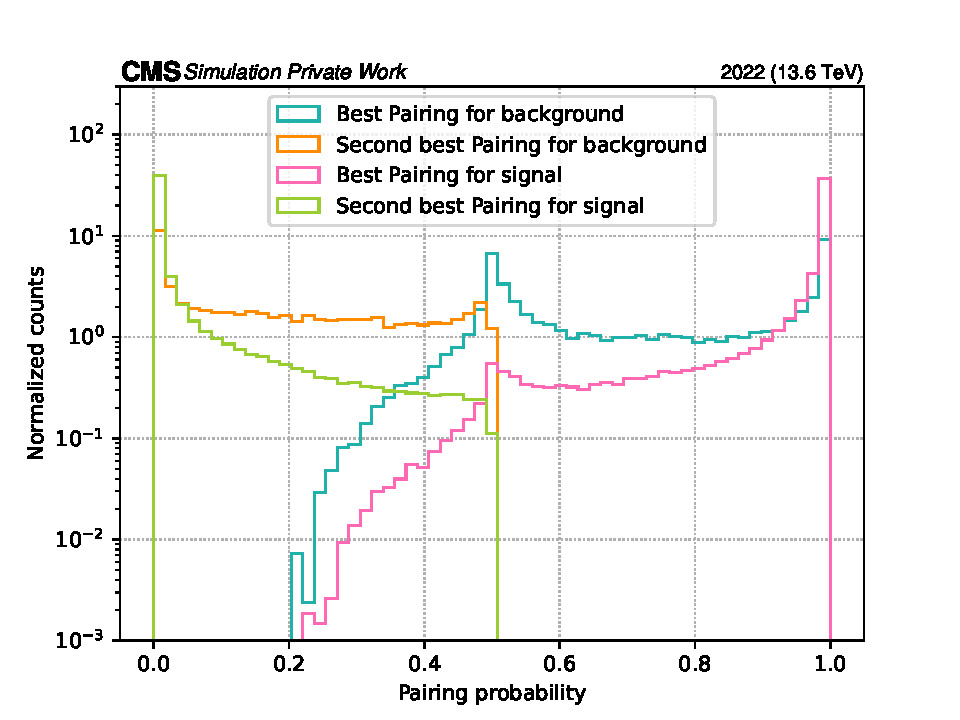
\includegraphics[width=0.7\linewidth]{Images/7.S:B/Prob diff/best_and_second_beest_pairings.pdf}
    \caption{Pairing probability distribution of the best and second-best pairings for signal and background events given by SPANet.}
    \label{fig: prob value}
\end{figure}

After evaluating a SPANet model on the test file, we obtain as output the pairing with the highest probability, i.e SPANet gives as output the pair of jets with the highest probability to be matched to the generator-level quarks coming from the decay of the leading and the sub-leading Higgs. This result is used in Section \ref{section: improving}. It is also possible to have as output the full matrix with all the pairing probabilities of the jets for the leading and the sub-leading Higgs, as illustrated in Figure \ref{fig: probabilities matrix}.


\begin{figure}[hbt]
    \centering
    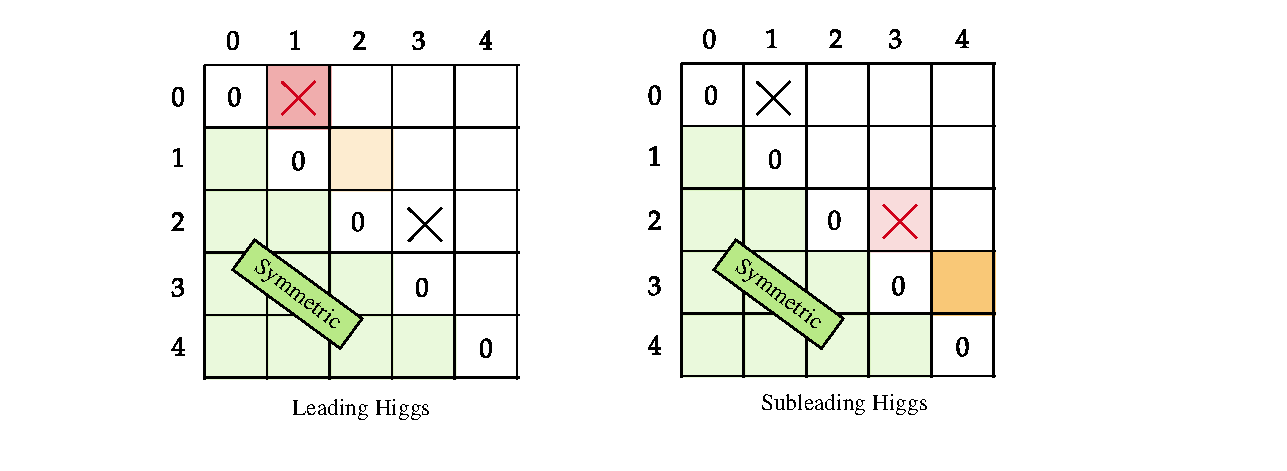
\includegraphics[width=0.8\linewidth]{Images/7.S:B/Prob diff/probability difference.pdf}
    \caption{Matrix of probabilities of the pairing of the jets. As 5 jets are considered for the pairing, we have a 5x5 matrix. The diagonal is 0, as a single jet cannot be paired with itself. This is a symmetric matrix as quarks from anti-quarks cannot be distinguished in the detector. In red, the highest pairing probabilities that are compatible are shown and the second highest are represented in orange.}
    \label{fig: probabilities matrix}
\end{figure}

Figure \ref{fig: probabilities matrix} shows a 5x5 matrix since we consider 5 jets for the pairing. Each entry of the matrix corresponds to the probability of matching these jets in the event together. Since it is impossible to pair a single jet with itself, the diagonal is 0. Due to the quark/antiquark symmetry of the pairing explained in Section \ref{subsection: run2 pairing} this matrix is symmetric.

To find the highest pairing probabilities, the SPANet pairing algorithm uses the overall highest probability, i.e. the highest probability in the leading or sub-leading Higgs matrices. In Figure \ref{fig: probabilities matrix}, the overall highest probability is shown in dark red. Once this probability has been found, the algorithm uses the subleading Higgs matrix in order to find the highest probability that is compatible with the first one, i.e. that does not share the same jets. The latter is shown in light red. In this example, it is observed that the matching is compatible since for the dark red the jets 0 and 1 are paired while for the light red, the jets 3 and 2 are paired. The next step to compute the PD variable is to find the second-best pairing in this matrix. To do so, firstly, the best pairings determined earlier are removed (red crosses). Moreover, the symmetric probabilities in the other matrix are removed (black crosses) as we have a symmetry between the leading and the sub-leading Higgs. Finally, the same procedure is applied to find the second-best pairing. In this second example, the highest second pairing is marked in dark orange. We find the complementary one on the other matrix in light orange.

To use this variable in the training, the best SPANet model presented in Section \ref{subsection: Optimal config} is evaluated on the signal and the background inputs that we will use to train the classifier. 
In Figures \ref{fig: 2b data PD}, \ref{fig: 2b QCD PD} and \ref{fig: 4b QCD PD} we show the PD variable for signal and background events. We observe the high discriminant power of this variable, especially in Figures \ref{fig: 2b data PD} and \ref{fig: 2b QCD PD} when considering the 2b data and 2b QCD as background in the SPANet training.

\begin{figure}[hbt]
    \centering
    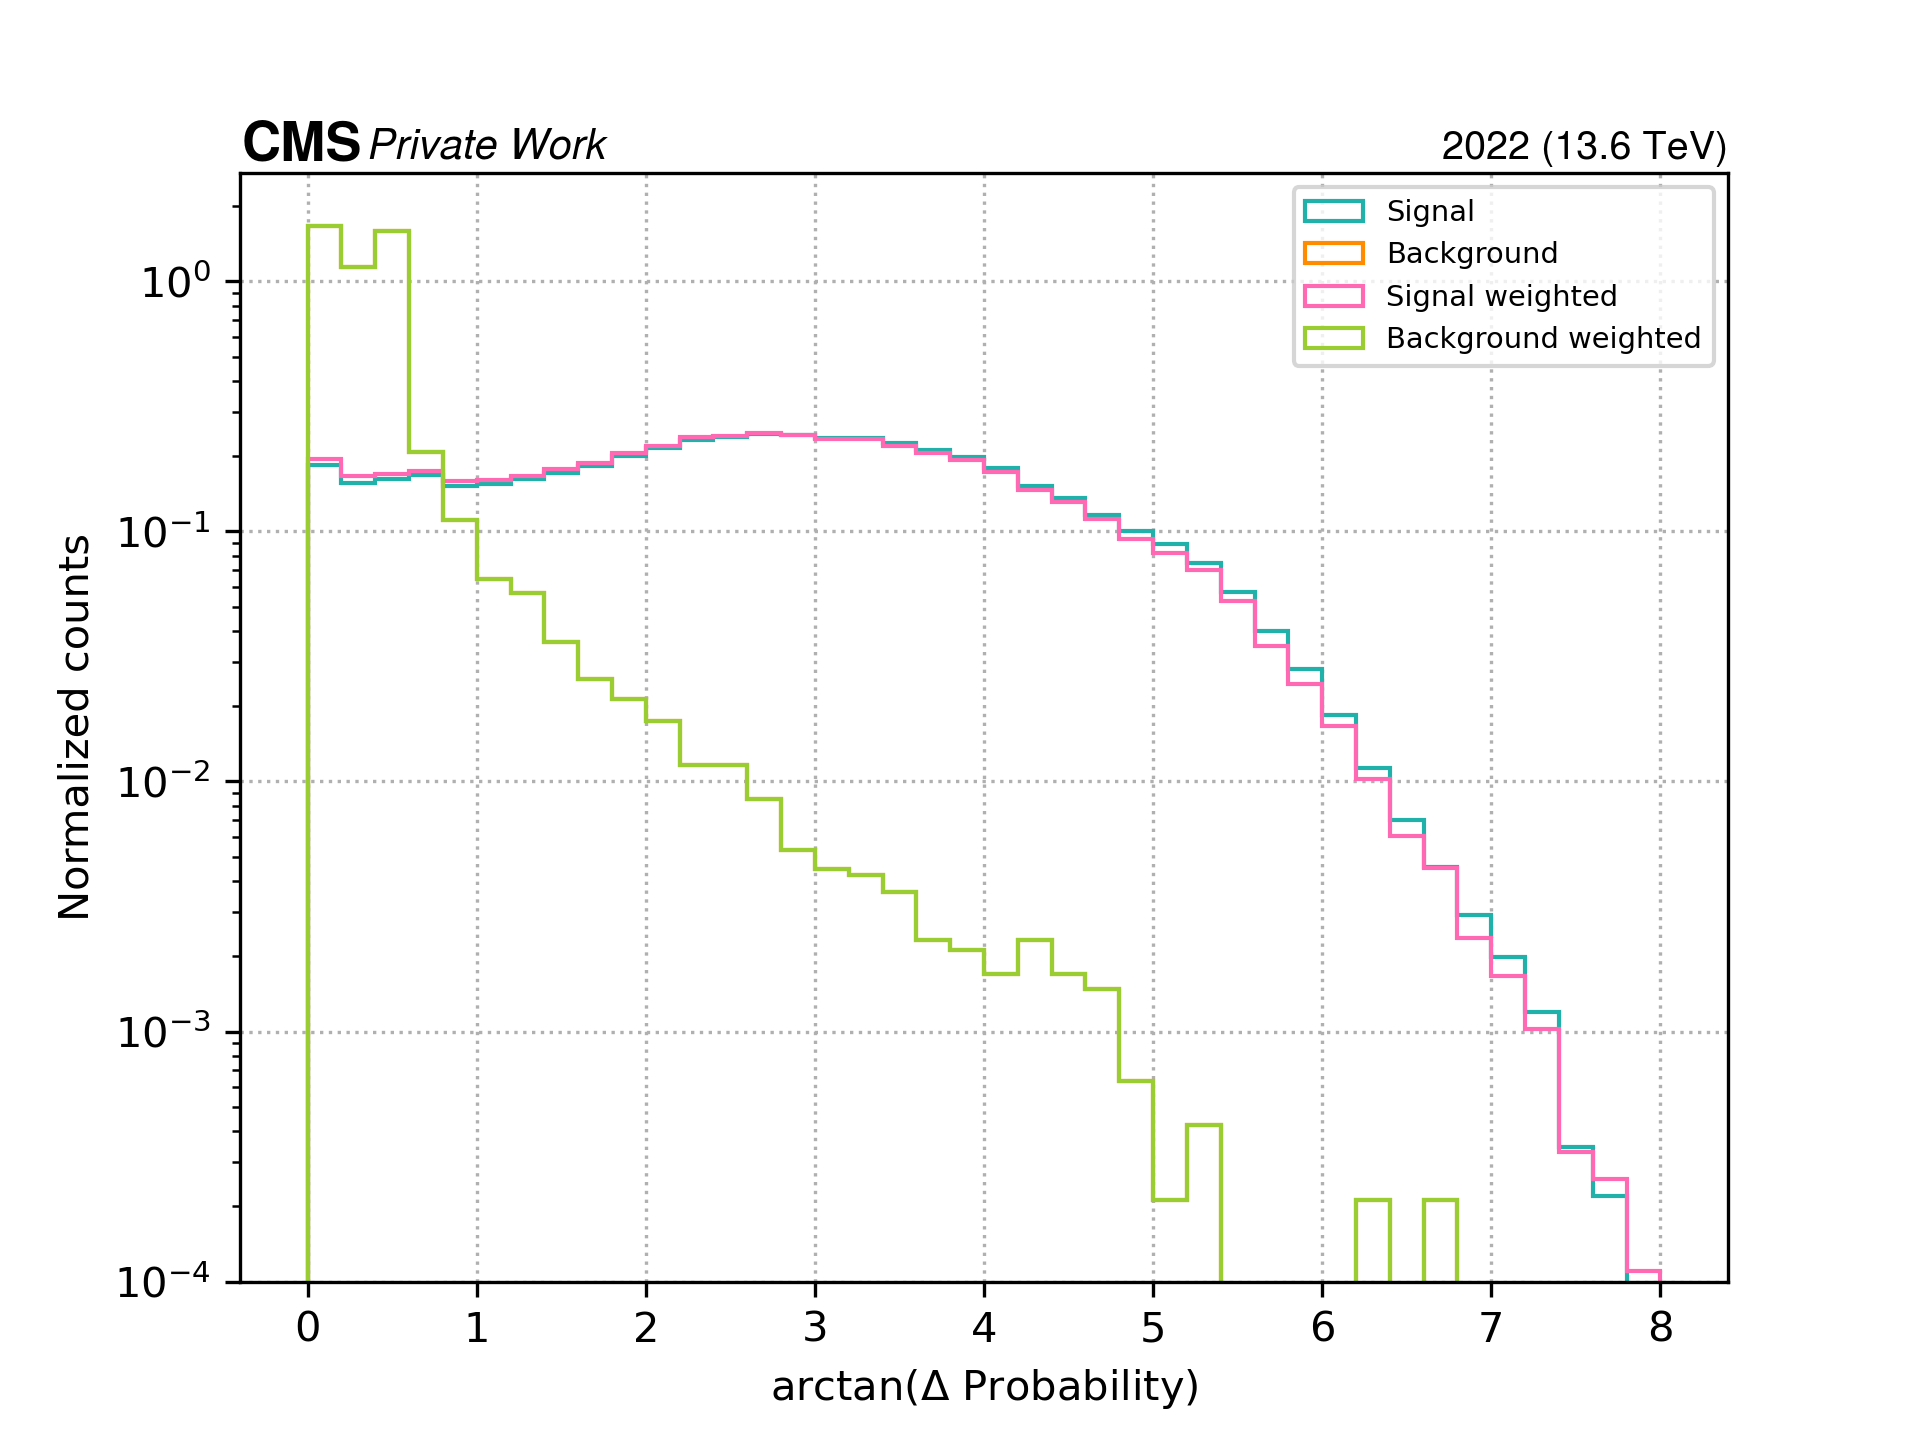
\includegraphics[width=0.7\linewidth]{Images/7.S:B/Prob diff/2b data reduced.png}
    \caption{Probability difference variable distribution in arc-tan used to extend the distributions, for signal and 2b data background events. The weighted and non weighted events, as mentioned in Section \ref{subsection: weights for the loss}, are shown. As this is a 2b data sample, the weighted and non weighted distributions are the same due to the definition of event weights.}
    \label{fig: 2b data PD}
\end{figure}

\begin{figure}
    \centering
    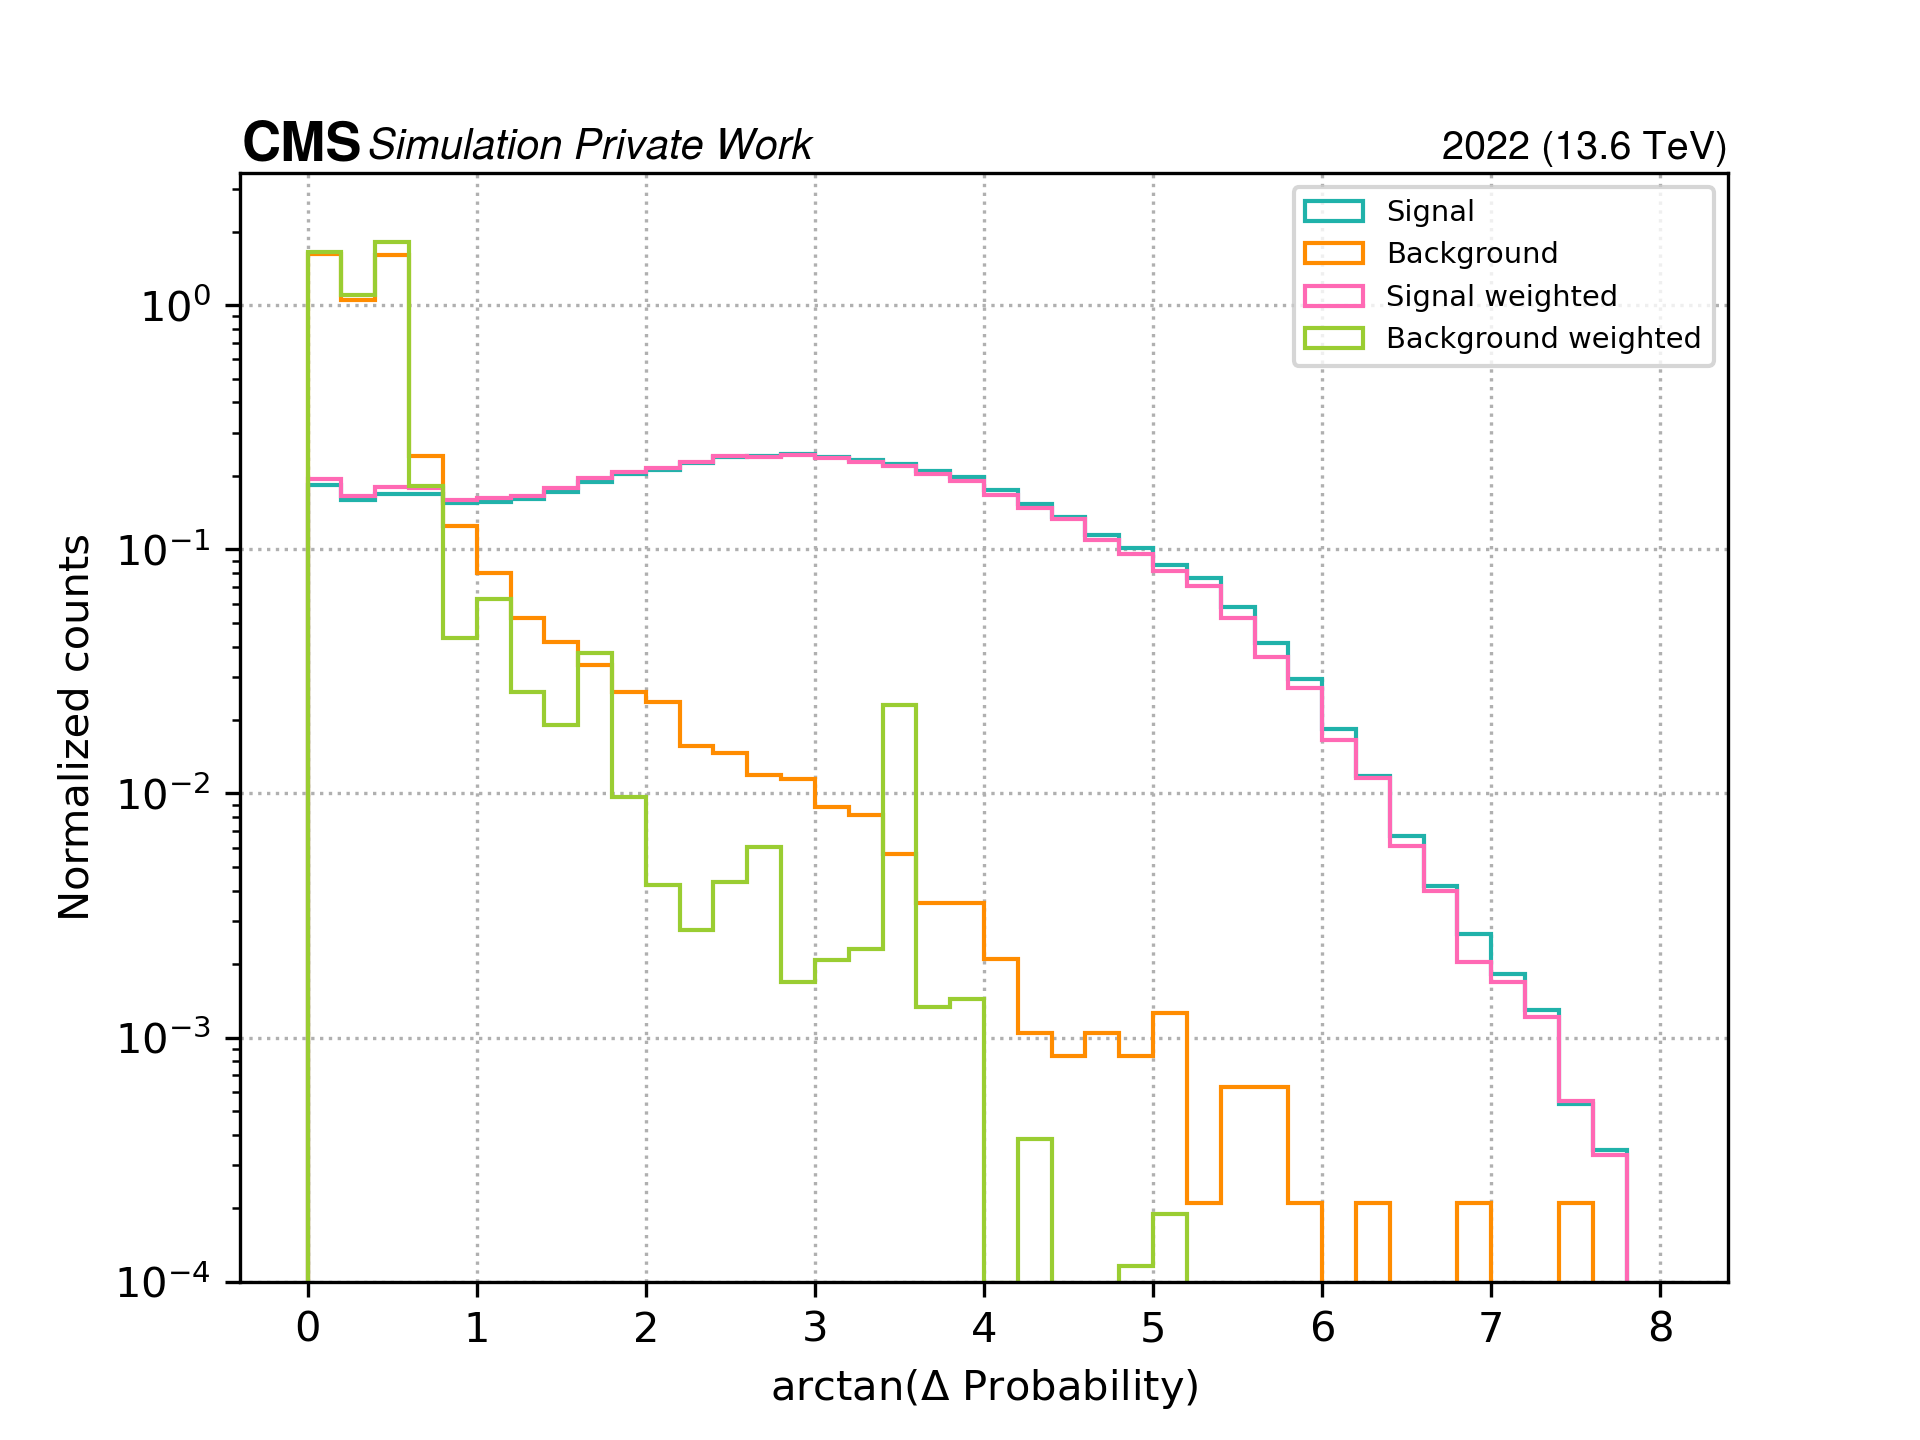
\includegraphics[width=0.7\linewidth]{Images/7.S:B/Prob diff/2b QCD arctan.png}
    \caption{Probability difference variable distribution in arc-tan used to extend the distributions, for signal and 2b data background events. The weighted and non weighted distributions are shown.}
    \label{fig: 2b QCD PD}
\end{figure}


\begin{figure}[hbt]
    \centering
    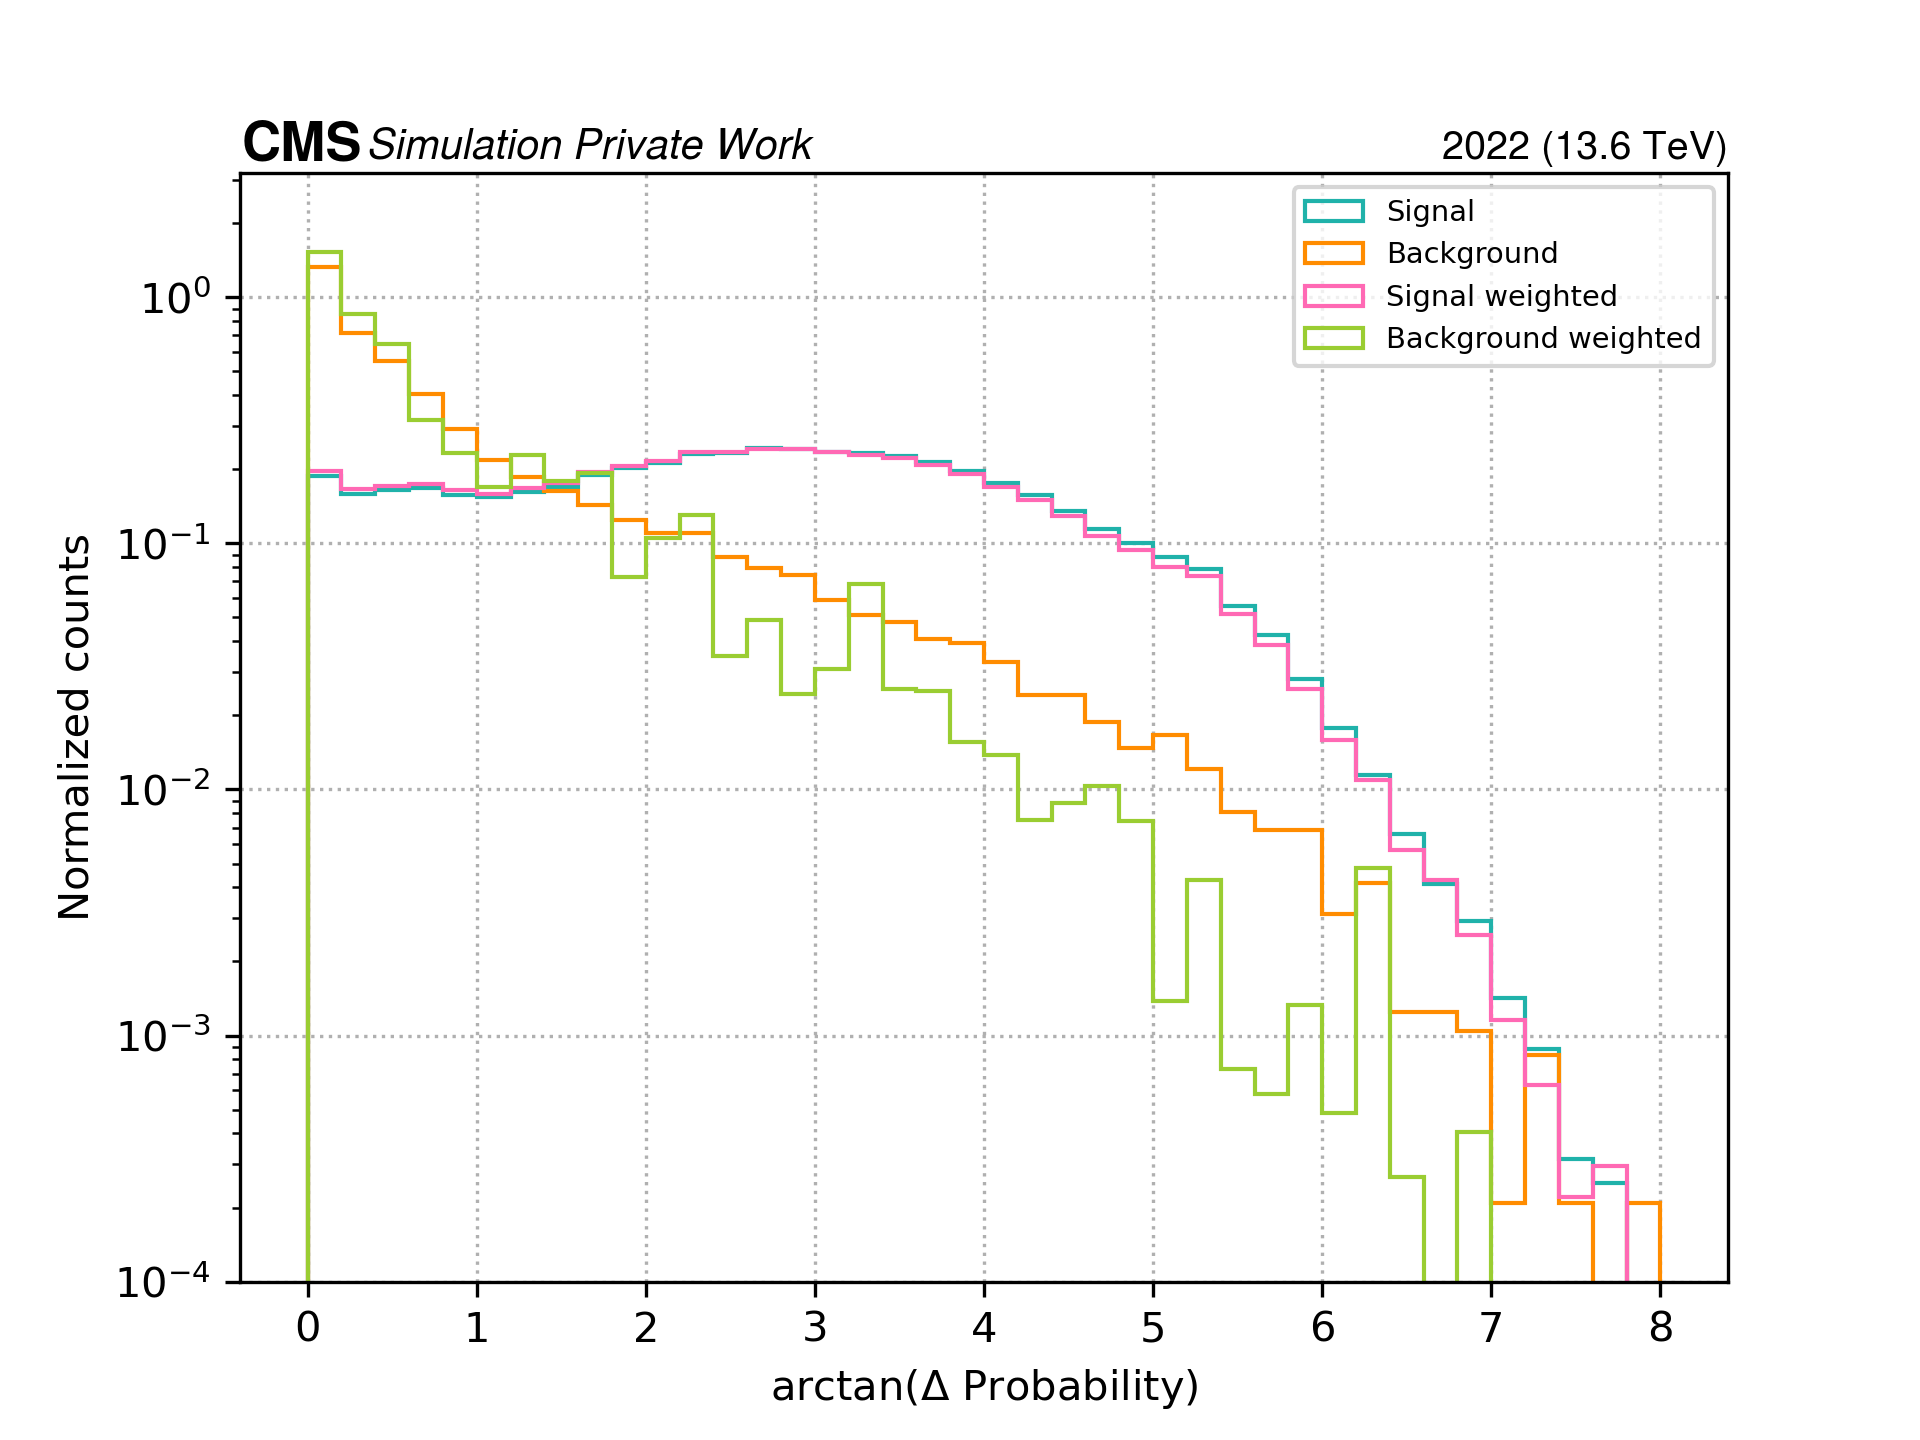
\includegraphics[width=0.7\linewidth]{Images/7.S:B/Prob diff/4b QCD arctan.png}
    \caption{Probability difference variable distribution in arc-tan used to extend the distributions, for signal and 2b data background events. The weighted and non weighted distributions are shown.}
    \label{fig: 4b QCD PD}
\end{figure}


Finally, as a figure of merit to assess the discriminating power of the PD variable, the Receiver Operating Characteristic (ROC) curve is used. The latter depicts the signal efficiency versus the misidentification rate of background events across various threshold selections. Figure \ref{fig: ROC PD} shows the weighted ROC curves of the probability difference distributions from Figures \ref{fig: 2b data PD}, \ref{fig: 2b QCD PD}, \ref{fig: 4b QCD PD}. In the latter, the False Positive Rate (FPR) refers to 1-$\epsilon_b$, with $\epsilon_b$ being the background efficiency taken as the fraction of background below the threshold. Finally, the True Positive Rate (TPR) refers to $\epsilon_s$, with $\epsilon_s$ being the signal efficiency taken as the fraction of background above the threshold. Figure \ref{fig: ROC PD} shows that for 2b data and 2b QCD an increase of FPR, at 90\% of signal efficiency. This is due to the fact that most of the background events have a highest best pairing probability of around 0.5 and the second best one has a value close to 0, therefore a peak of events is observed at $\Delta$Probability = 0.5, which corresponds to 90\% of signal efficiency and explains this feature in the ROC curve for FPR=90\%.

\begin{figure}
    \centering
    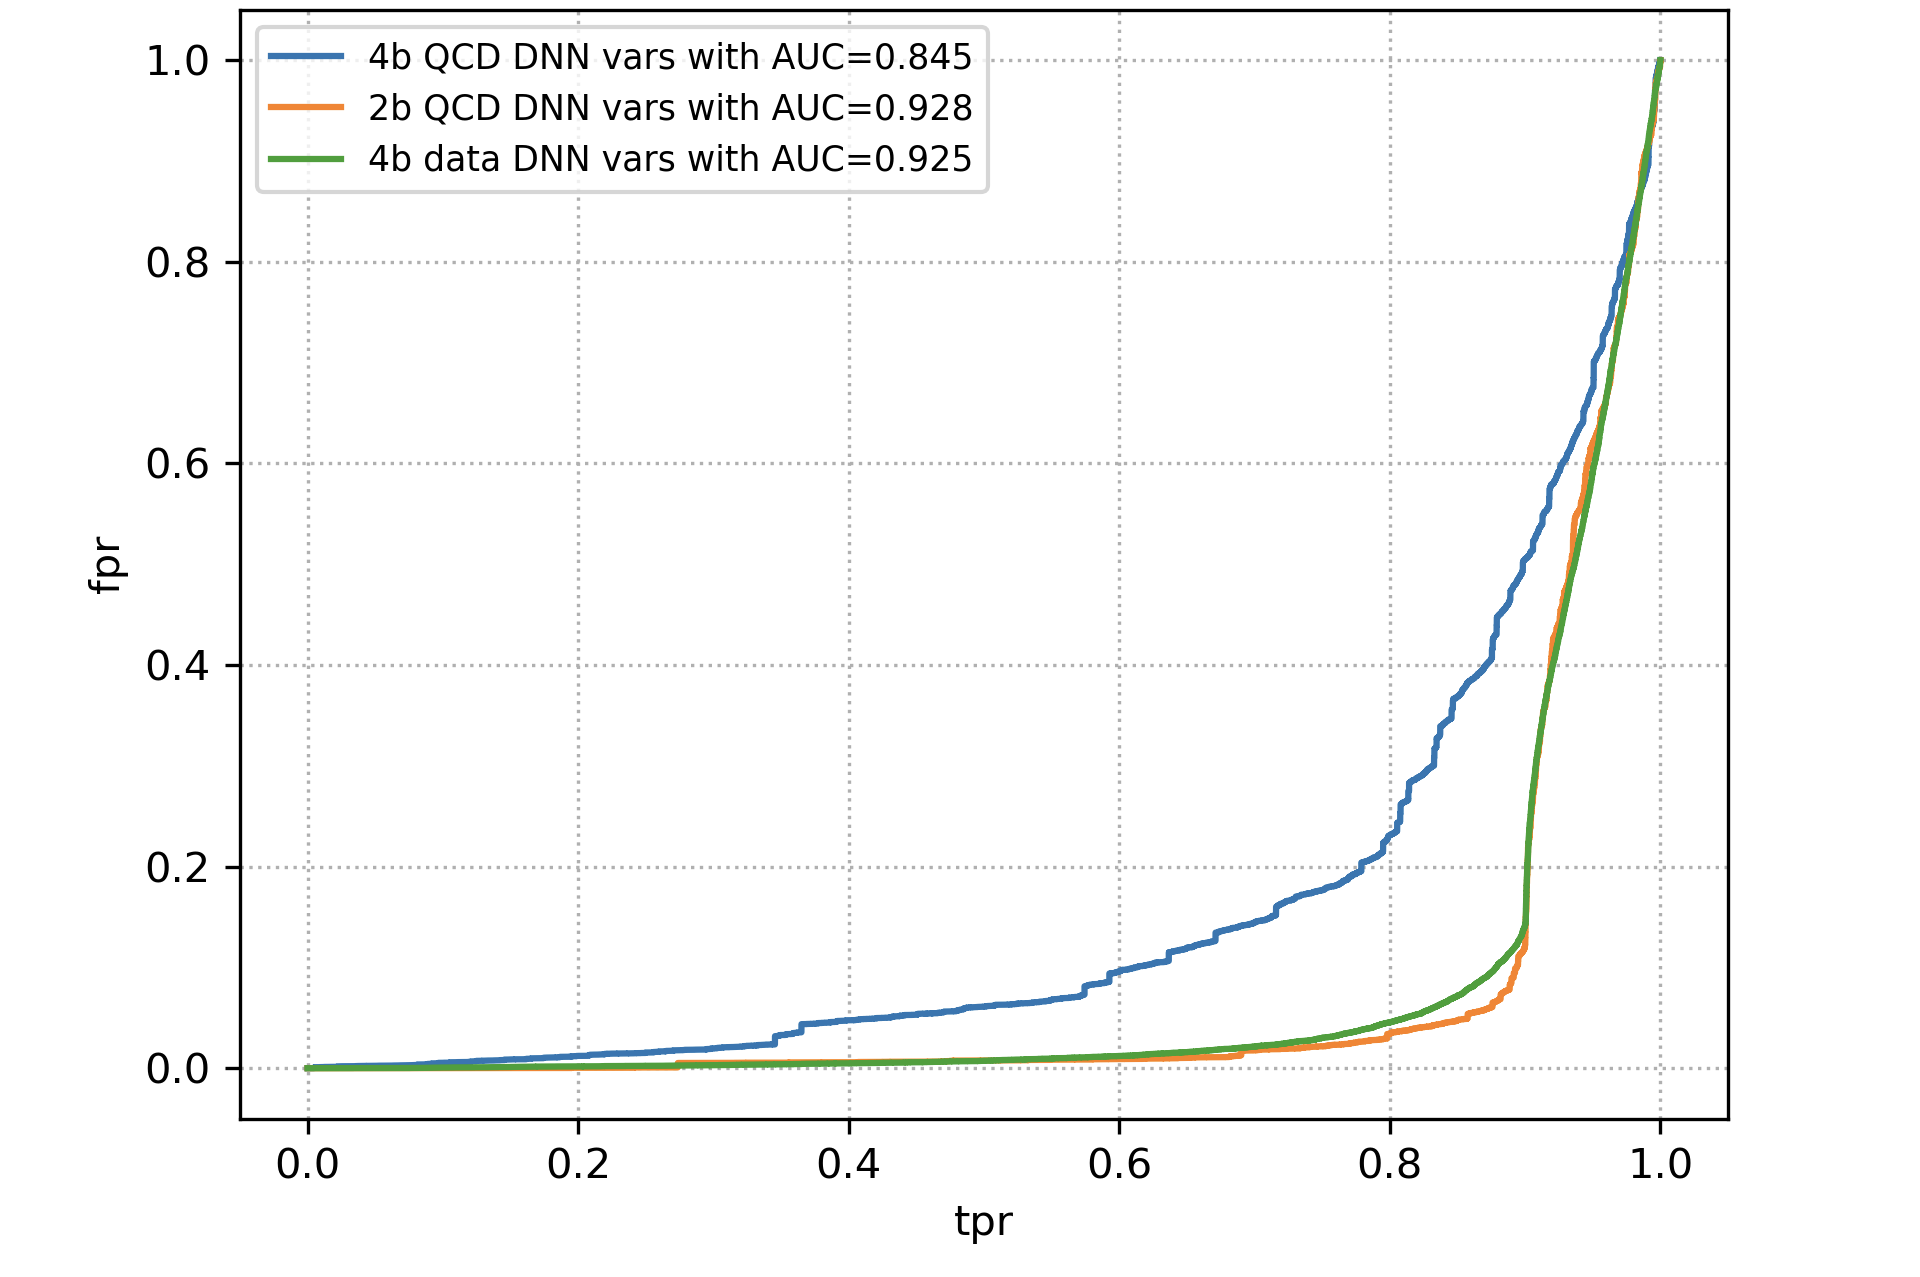
\includegraphics[width=0.7\linewidth]{Images/7.S:B/Prob diff/Probability difference ROC curve.png}
    \caption{Weighted ROC curves of the probability difference variables distributions shown in Figures \ref{fig: 2b data PD}, \ref{fig: 2b QCD PD} and \ref{fig: 4b QCD PD} for 2b data, 2b QCD and 4b QCD. The AUC of these ROC curves is also reported in the plot.}
    \label{fig: ROC PD}
\end{figure}

\clearpage

\subsection{Sample dependency} \label{subsection: sample dep}

As mentioned earlier, it would be optimal to use 4b morphed data for the SPANet training. Nevertheless, as this is not possible yet, the 4b data performance will be assessed differently using three different configurations presented later in the text. These configurations are given by either using 4b QCD, 2b QCD, or 2b data, defined in Section \ref{subsubsecxtion: 4/2 b regions} as background samples. We will refer to each configuration in the following by the name of the sample used for the background in the training. For each configuration, we will be comparing the training using only DNN variables as inputs or DNN and PD variables.

In order to have a meaningful comparison to the performance of the DNN used in Run 3 presented in the AN \cite{ANRun3} where the 4b morphed data is used for the training, the results of the SPANet training will be inferred in the 4b data. To do so, we will infer the value of the area under the curve (AUC) by using the following expression:

\begin{equation}
    \text{AUC}(\text{4b-data})= \text{AUC}(\text{2b-data}_f) \times {\frac{\text{AUC}(\text{4b-QCD})}{\text{AUC}(\text{2b-QCD}_r)}} \times {\frac{\text{AUC}(\text{2b-QCD}_r)}{\text{AUC}(\text{2b-data}_r)}}
    \label{eq: extrapolation}
\end{equation} 
\noindent Since the 4b morphed data and the 2b data have the same number of events, the value of the AUC of the 2b data full statistics (black) is used. The $f$ in Eq.(\ref{eq: extrapolation}) refers to same with full statistics. In order to infer SPANet predictions from 2b to 4b data, the ratio 4b/2b accounts for the b-tag dependency of the SPANet model. This value will be given by the first ratio (${\frac{\text{AUC}(\text{4b-QCD})}{\text{AUC}(\text{2b-QCD}_r)}}$). Nevertheless, this b-tag ratio is computed using QCD MC samples, therefore the additional dependency on the sample (QCD vs data sample) needs to be accounted for as well. This is encapsulated in the second ratio term (${\frac{\text{AUC}(\text{2b-QCD}_r)}{\text{AUC}(\text{2b-data}_r)}}$). Finally, both ratios have been extracted using a reduced dataset (marked with $r$ in Eq.(\ref{eq: extrapolation})). As we aim to probe the b-tag dependency and the model dependency, we perform a random removal of events so that the effective statistics of numerator and denominator is the same and therefore do not play any role in the comparison. The statistics of the 4b data ($\sim$ 100k events) will be used since it is the dataset with the lowest number of events.

In order to infer the ROC curve, Eq.(\ref{eq: extrapolation}) is used to compute the value of the FPR instead of the AUC. Nonetheless, applying Eq.(\ref{eq: extrapolation}) to the TPR as well will result in a linear rescaling of the 2b data ROC curve and not the ROC curve inferred for the 4b data. However, if a training using 4b morphed data is performed, the signal sample would be the same used for the 2b data trainings thus the TPR values would remain similar. Therefore to obtain the inferred 4b data ROC curve the TPR values from the 2b data ROC curve are used and only the FPR is modified.

%The final goal is to infer the 4b data ROC curve which will be shown in Sections \ref{subsection:4b data extrapolation inclusivce} and \ref{subsubsection: train and eev on SR}. However, as discussed in Eq.(\ref{eq: extrapolation}) the results of the trainings with 4b-QCD, 2b-QCD reduced statistics, 2b-data reduced statistics and 2b-data full statistics are needed to infer this result.


\subsection{Results on the input comparison} \label{subsection: results on the trainings}

%Compare weighted and non weighted
%also for the SPANet

In this Section, we will present the results of the trainings using the 2b data, 2b QCD, and 4b QCD configurations. In Figures \ref{fig: 4b QCD comp input}, \ref{fig: 2b QCD comp input} and \ref{fig: 2b data comp input} we show the weighted ROCs of these trainings. It is observed that for 2b-QCD (Fig.\ref{fig: 2b QCD comp input}) and 2b-data (Fig.\ref{fig: 2b data comp input}) samples, adding the PD variable results in a significant improvement of the classification performance. For the 4b-QCD configuration (Fig. \ref{fig: 4b QCD comp input})  the performance is only slightly increased.  The difference in the improvement when adding the PD variable between 4b and 2b can be explained by looking at Figures \ref{fig: 2b data PD}, \ref{fig: 2b QCD PD} and \ref{fig: 4b QCD PD}, where it is observed that the discriminating power of the PD variable is lower when using 4b-QCD. Nevertheless, after performing several tranings, a variability impacting the performance is observed. This will be quantitatively discussed in Section \ref{subsection: var of training S/B}.


\begin{figure}[hbt]
    \centering
    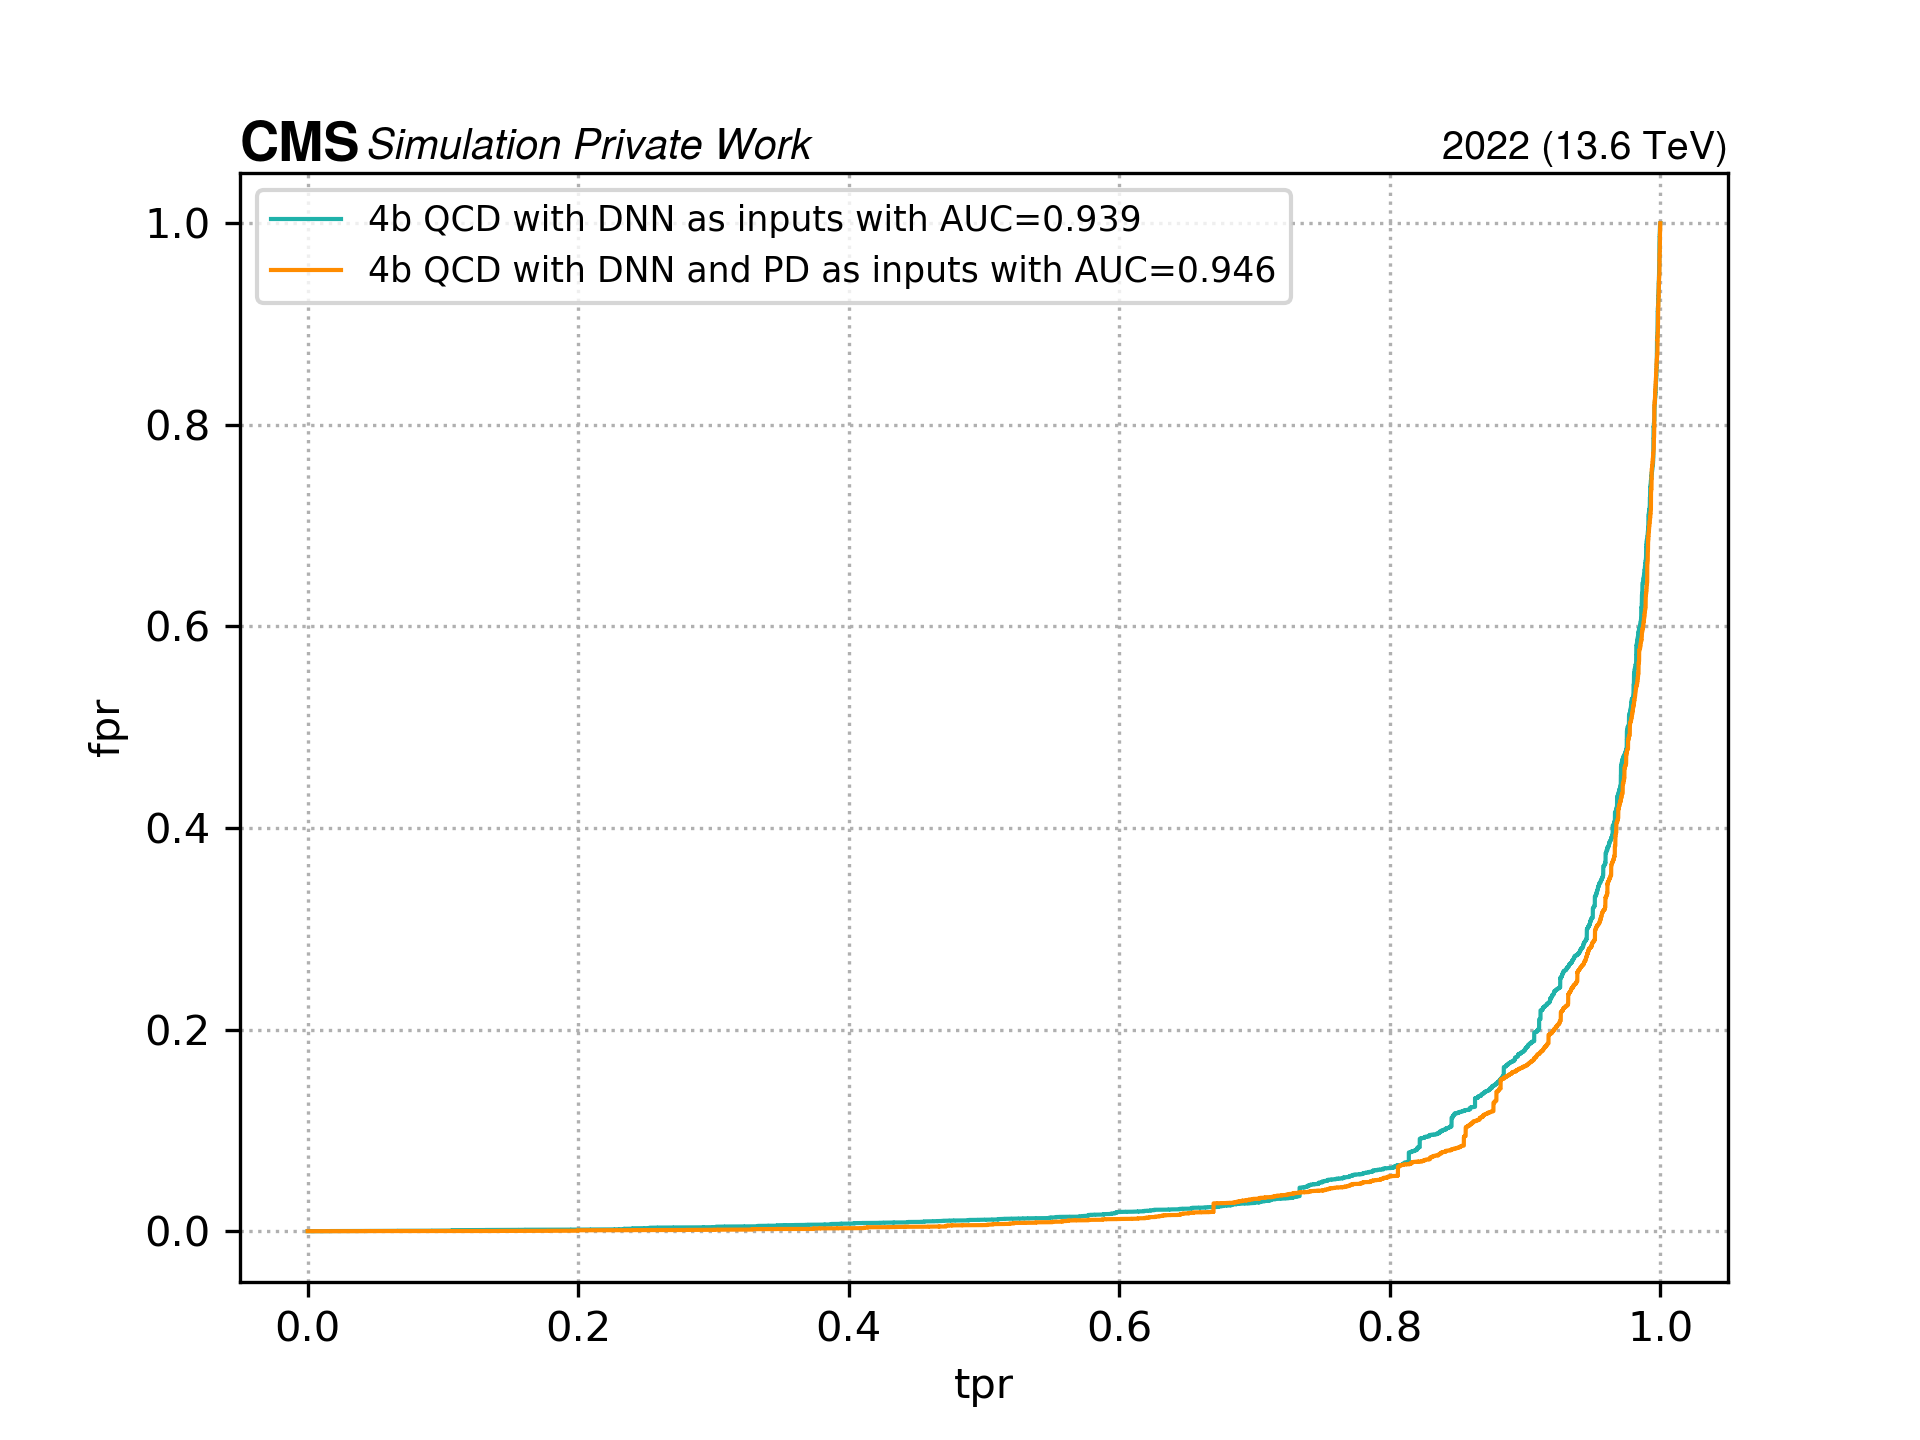
\includegraphics[width=0.7\linewidth]{Images/7.S:B/Inputs/4b QCD bis.png}
    \caption{Weighted ROC curves of the 4b-QCD configuration comparing the performance using different global inputs (DNN vs DNN and PD).}
    \label{fig: 4b QCD comp input}
\end{figure}

\begin{figure}[hbt]
    \centering
    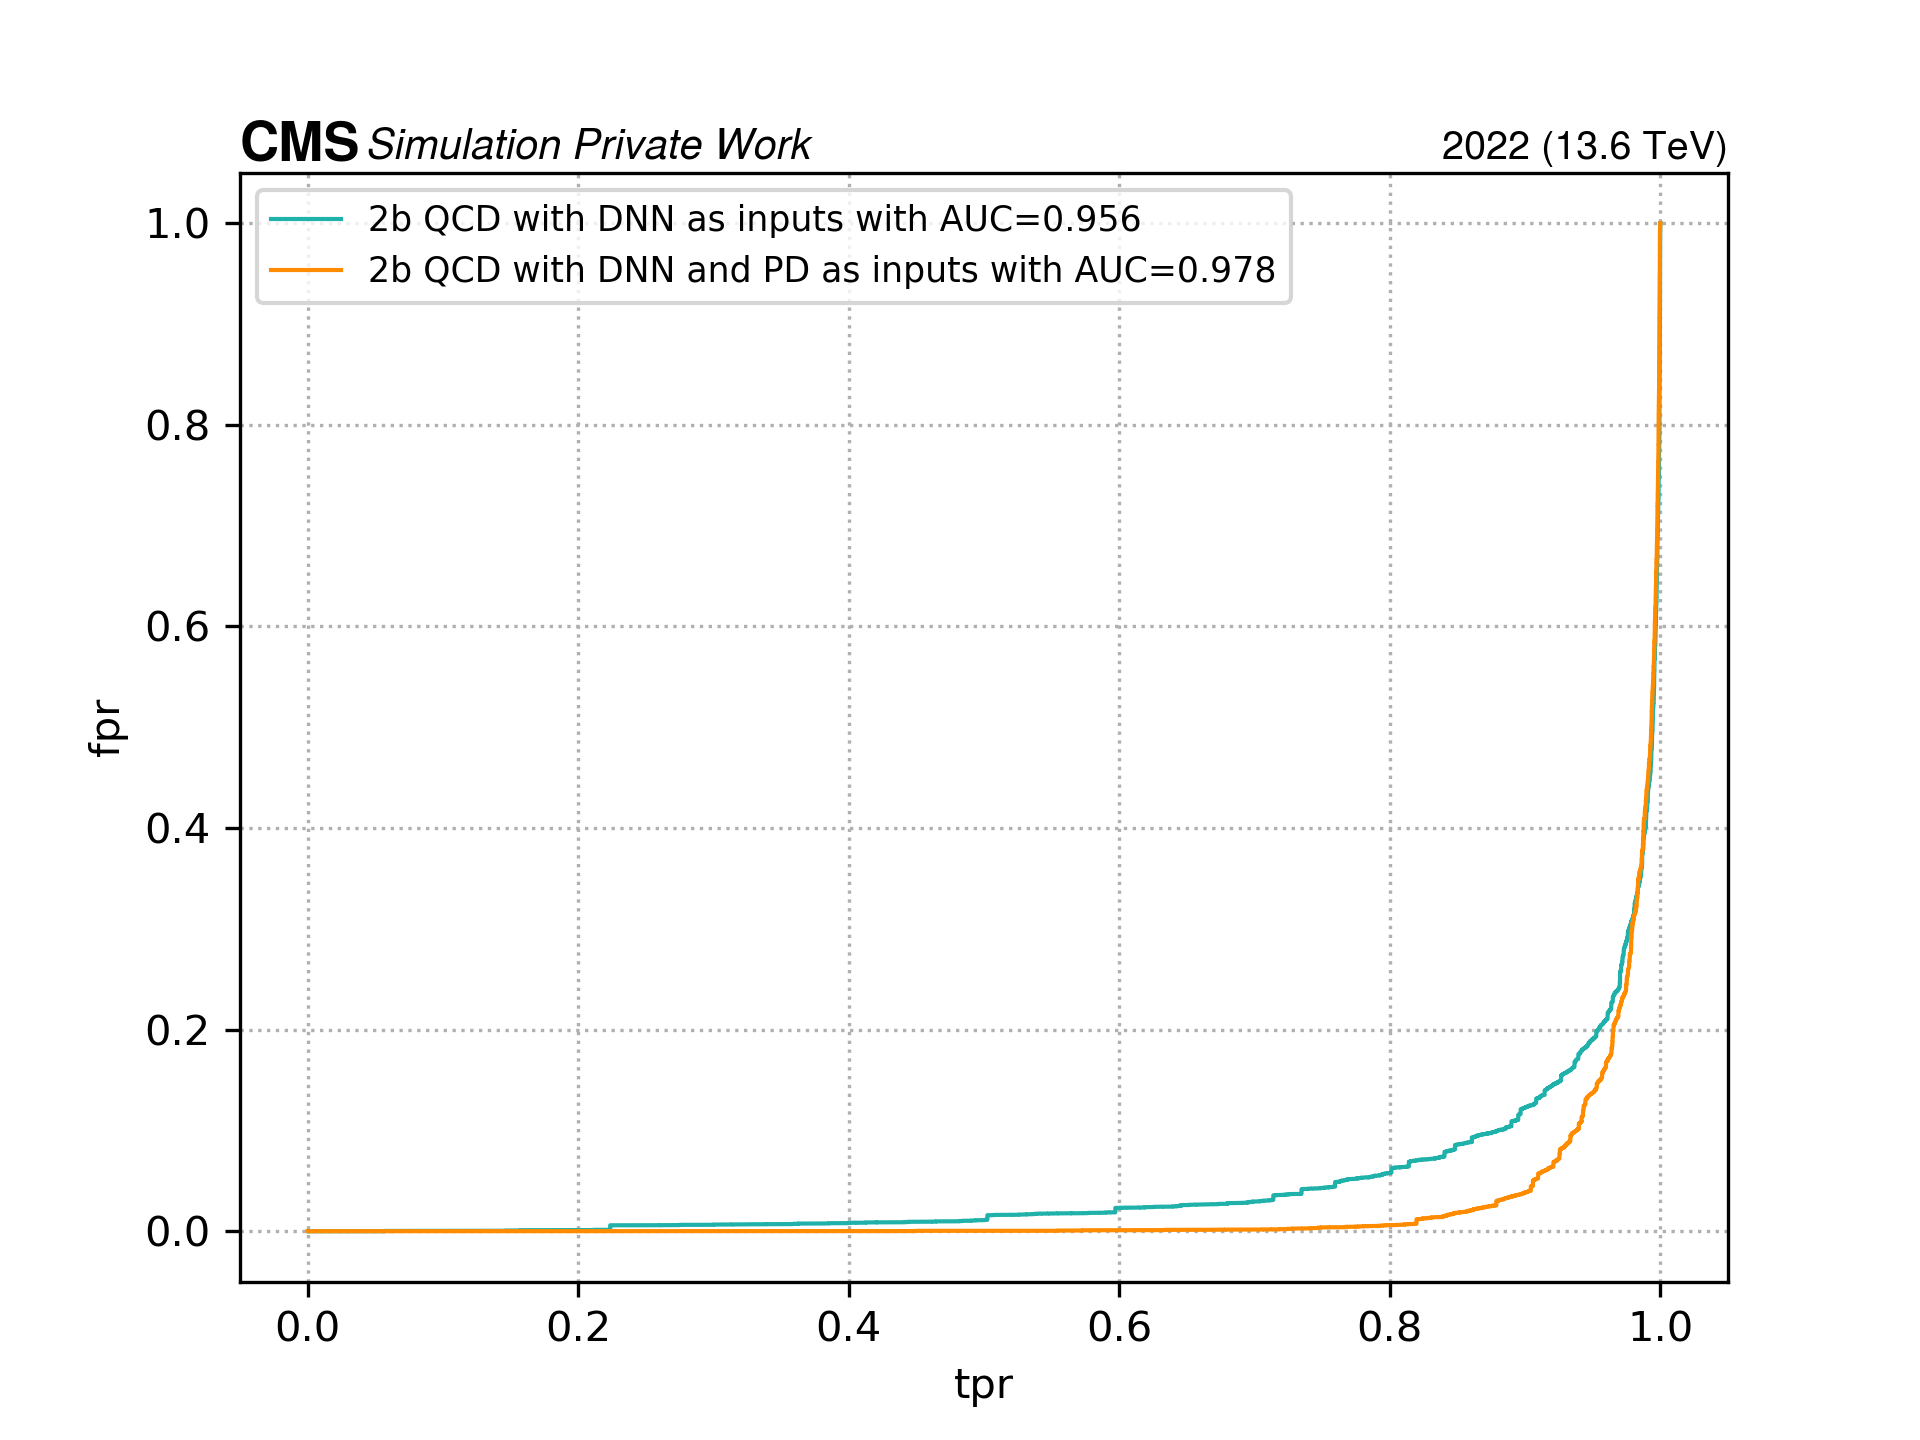
\includegraphics[width=0.7\linewidth]{Images/7.S:B/Inputs/2b QCD.png}
    \caption{Weighted ROC curves of the 2b-QCD configuration comparing the performance using different global inputs (DNN vs DNN and PD).}
    \label{fig: 2b QCD comp input}
\end{figure}

\begin{figure}[hbt]
    \centering
    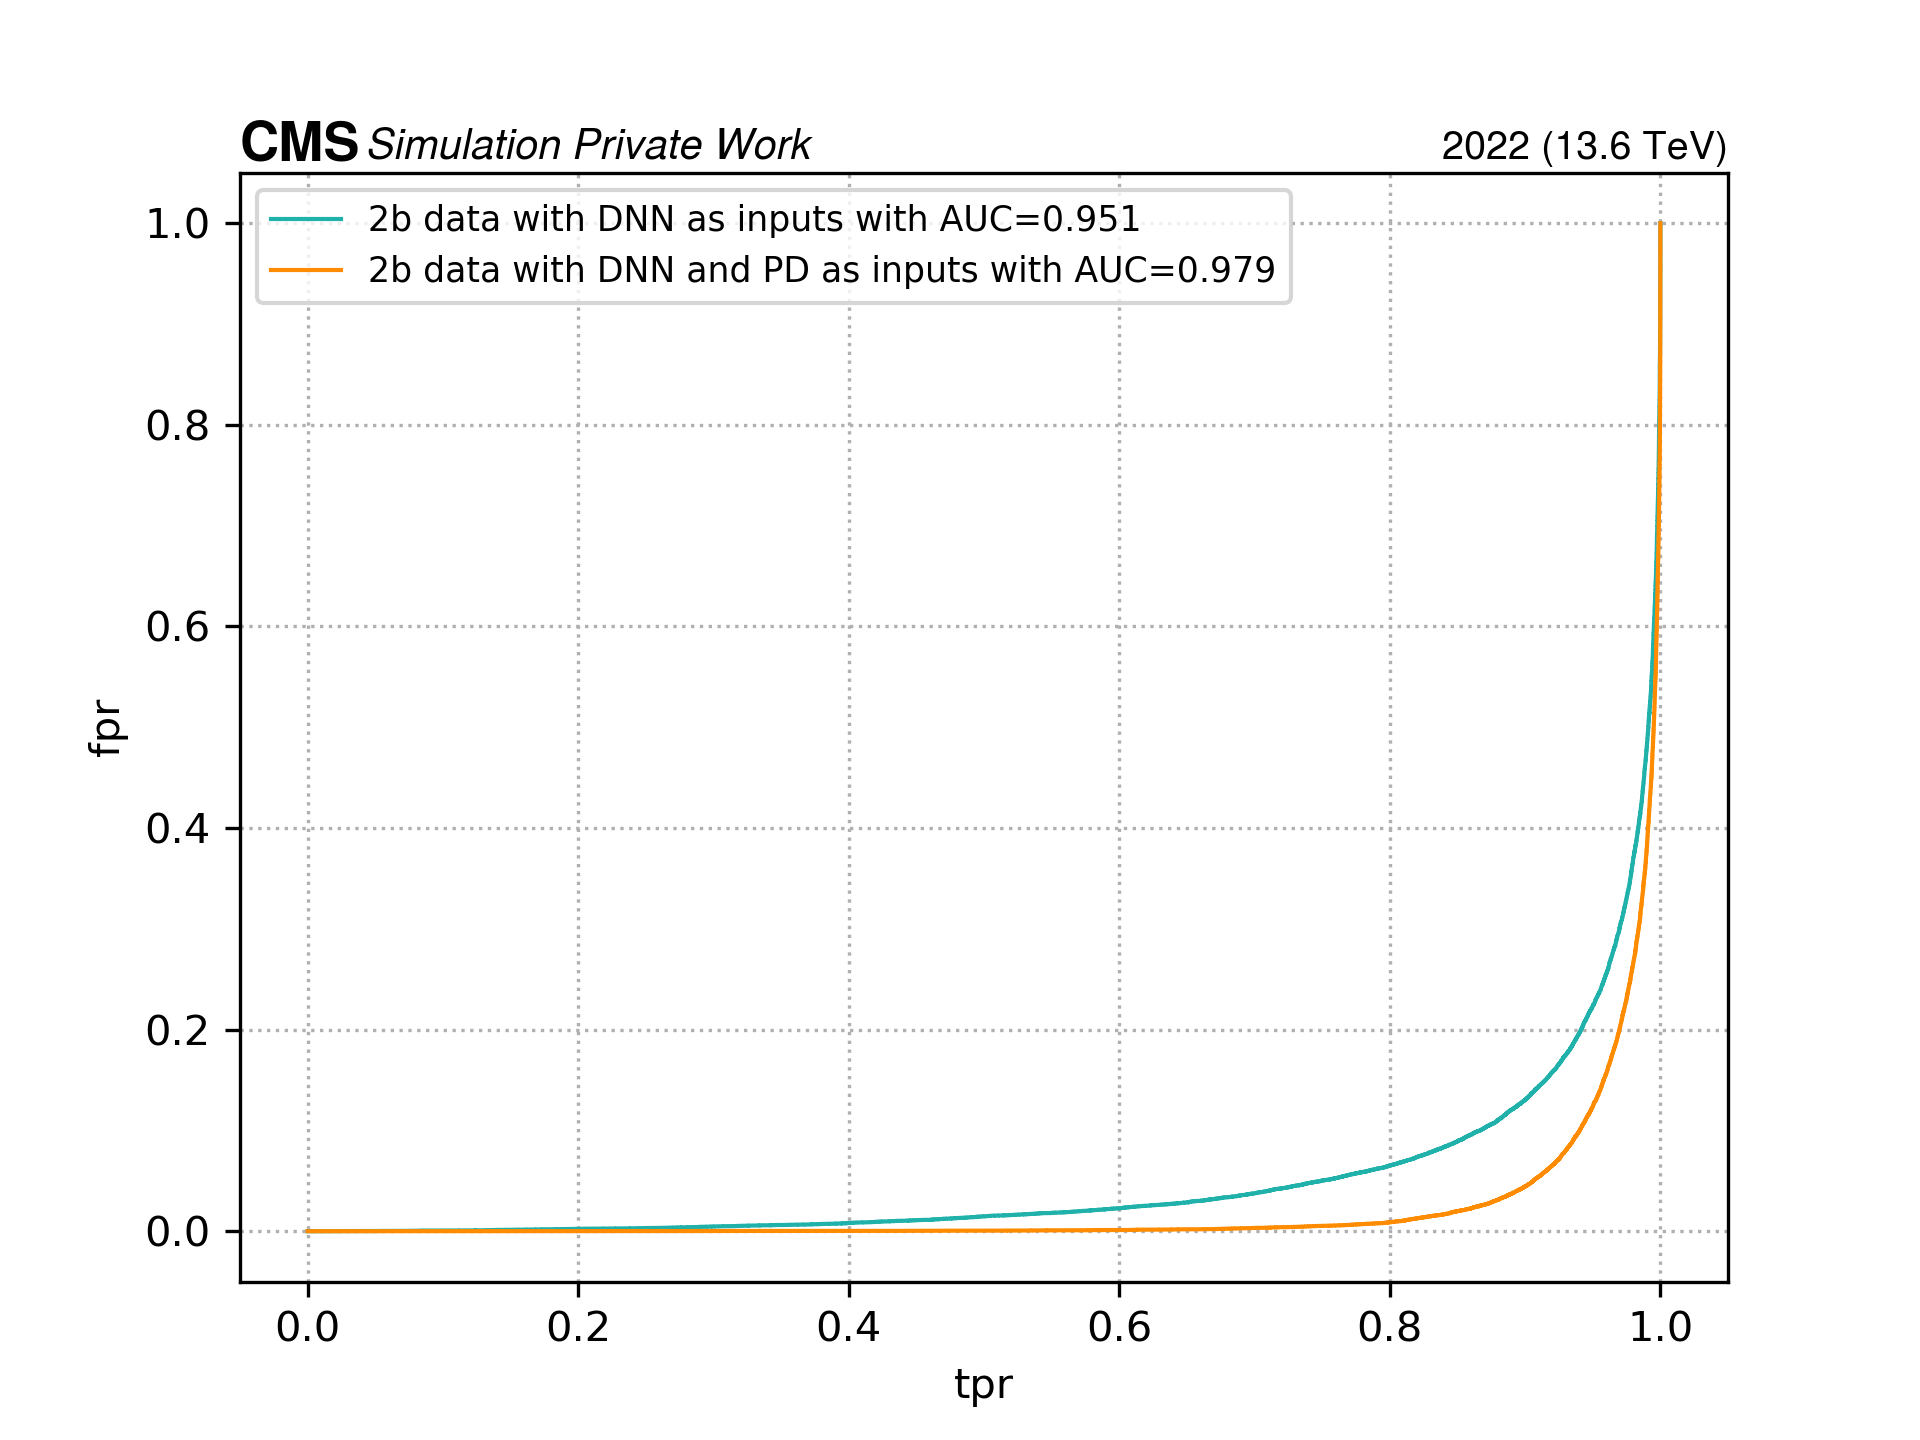
\includegraphics[width=0.7\linewidth]{Images/7.S:B/Inputs/2b data.png}
    \caption{Weighted ROC curves of the 2b-data configuration comparing the performance using different global inputs (DNN vs DNN and PD).}
    \label{fig: 2b data comp input}
\end{figure}

Finally, the non weighted ROC for the 4b-QCD configuration is shown. Figure \ref{fig: 4b QCD ROC no weights} shows that the distribution is smoother compared to the ROC curves in Figure \ref{fig: 4b QCD comp input}. This feature is explained by looking at the SPANet output of the classification in Figure \ref{fig: SPANet output S/B 4b QCD}: adding the weights adds fluctuations to the SPANET score distribution which are reflected in the ROC curve. Nevertheless, in the following, only the weighted ROC curves will be shown as they allow a meaningful treatment of the signal/background components in the training.

\begin{figure}[hbt]
    \centering
    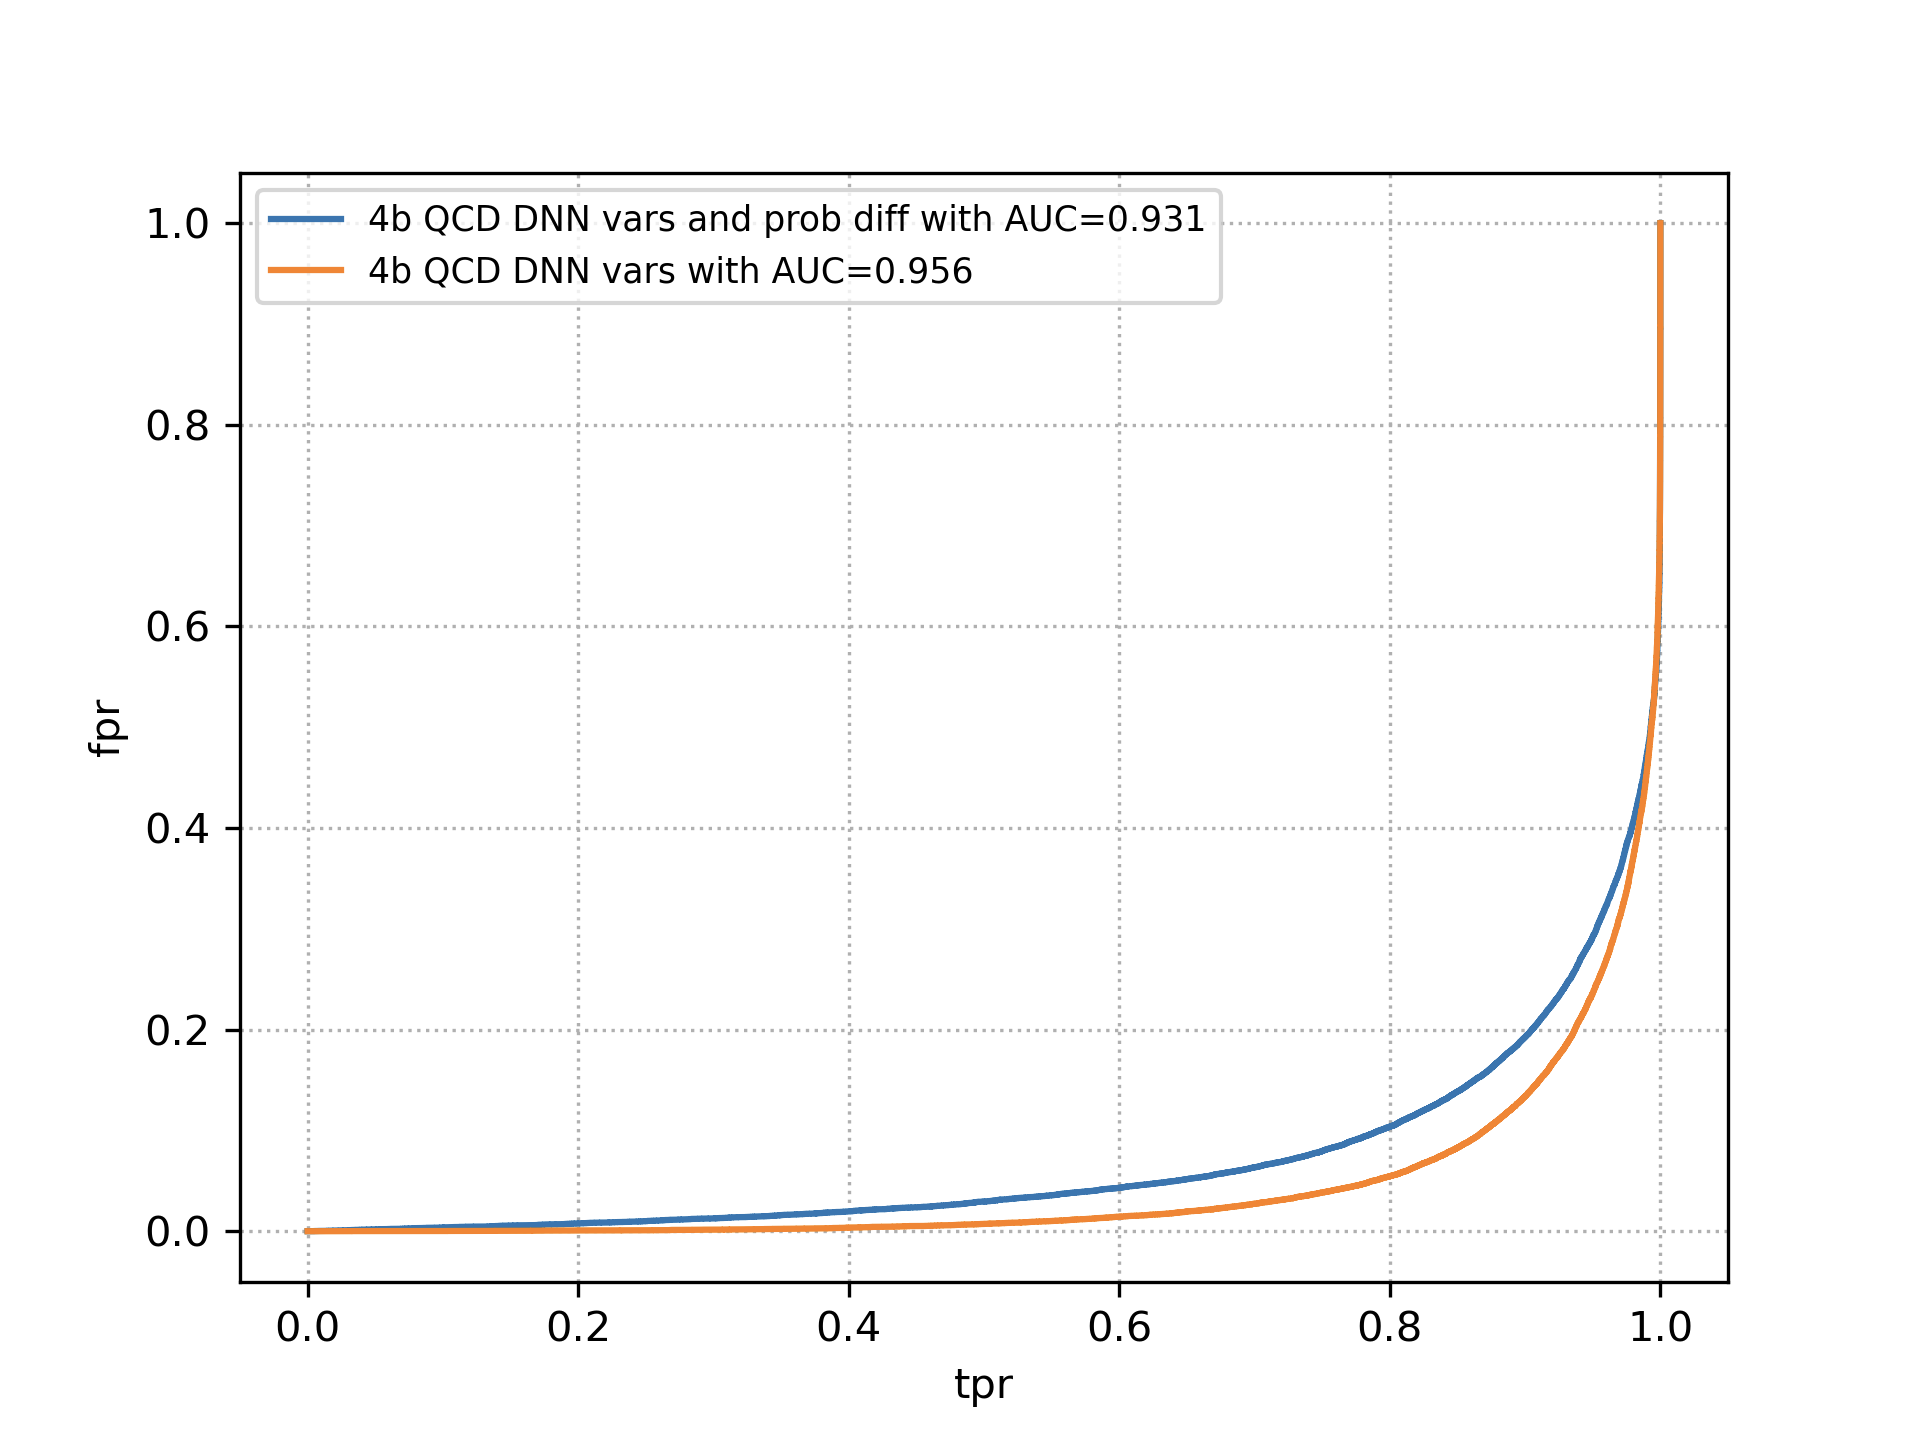
\includegraphics[width=0.7\linewidth]{Images/7.S_B/Inputs/no weights 4b QCD.png}
    \caption{Unweighted ROC curves of the 4b-QCD configuration comparing the performance using different global inputs (DNN vs DNN and PD).}
    \label{fig: 4b QCD ROC no weights}
\end{figure}

\begin{figure}
    \centering
    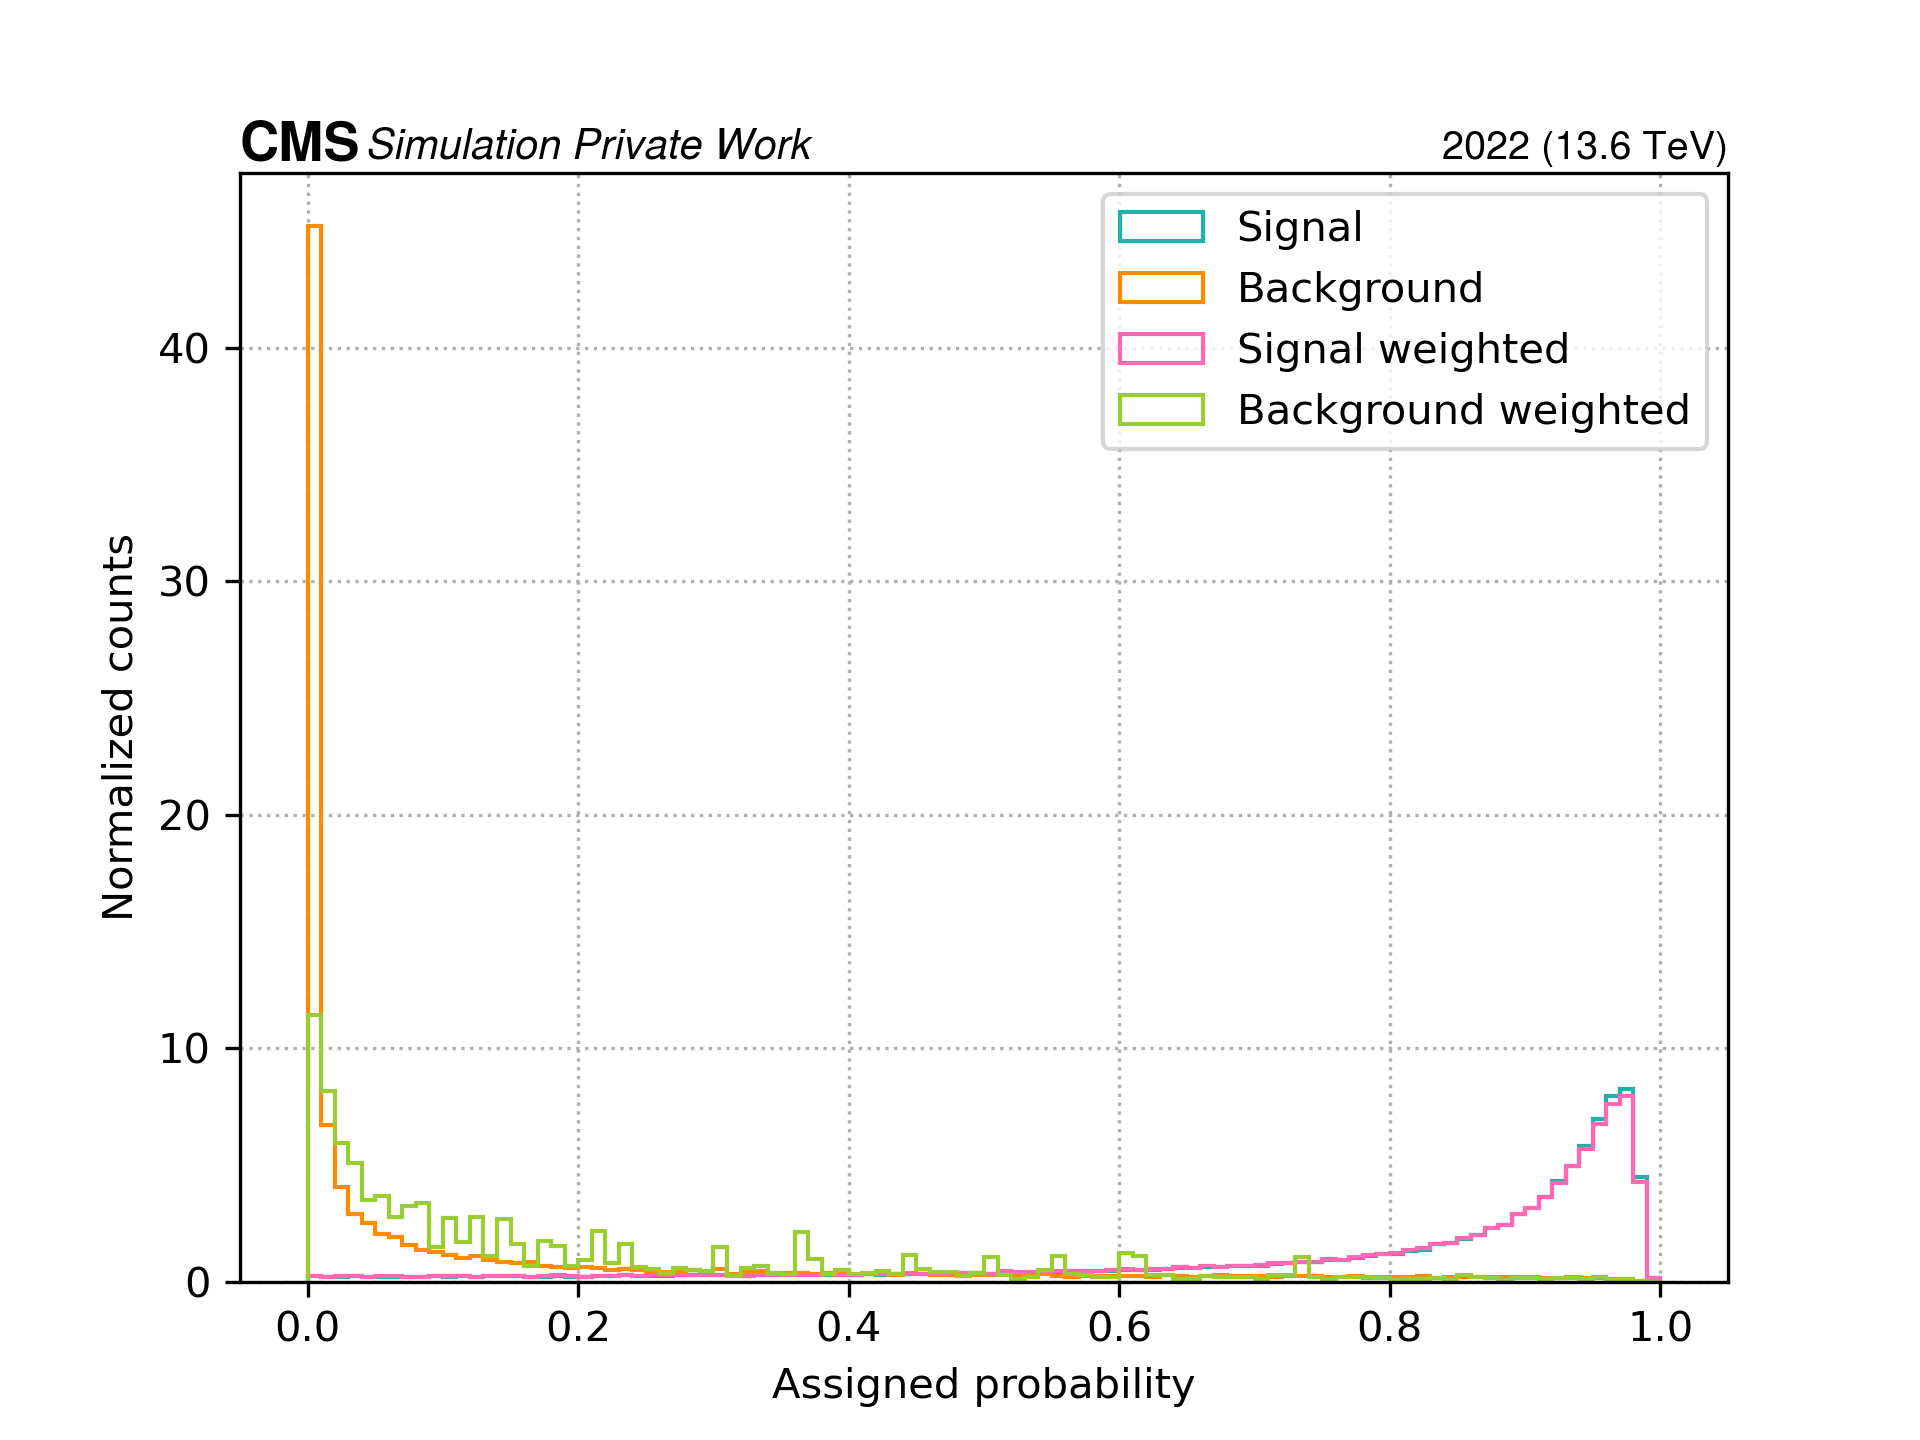
\includegraphics[width=0.7\linewidth]{Images/7.S:B/Classification outputs/4b QCD dnn.png}
    \caption{SPANet output for the classification training using the 4b QCD configuration and DNN as input variables. The probability assigned to the signal events and to the background events are shown. Significant differences are observed for the background SPANET output scores when applying the weights.}
    \label{fig: SPANet output S/B 4b QCD}
\end{figure}

\clearpage

\subsection{Assessing the variability of the trainings} \label{subsection: var of training S/B}

Unlike in Section \ref{subsection: pairing variability}, in the current Section, we assess the variability of the performance by using ROC curves as a figure of merits instead of validation accuracies. However, similarly to the studies performed in Section \ref{subsection: pairing variability}, different trainings using the same configuration but fixing eleven different seeds to randomly initialize the weights are performed. Figures \ref{fig: 4b QCD v ariability}, \ref{fig: 2b QCD v ariability}, \ref{fig: 2b data v ariability} show the results of these trainings. A summary of the AUC values observed in these Figures is reported in Table \ref{table: Spread of the trainings}. It is observed that the variability using 2b-QCD and 2b-data configurations is less than 0.02, as it is for 4b-QCD using DNN variables as inputs. Nevertheless, for 4b-QCD using DNN and PD as inputs we find a large variability. This large variability seen in Figure \ref{fig: 4b QCD DNN PD}, explains the features regarding the performance comparisons discussed in Section \ref{subsection: results on the trainings}. Therefore, we conclude that the SPANET performance using 4b QCD with DNN and PD variables is the same within the variability range of the training with respect to the SPANET training only using DNN variables.
% ases tghe variability by looking at the AUCs (before: first thing)

\begin{figure}[hbt]
\centering
\begin{subfigure}{.5\textwidth}
  \centering
  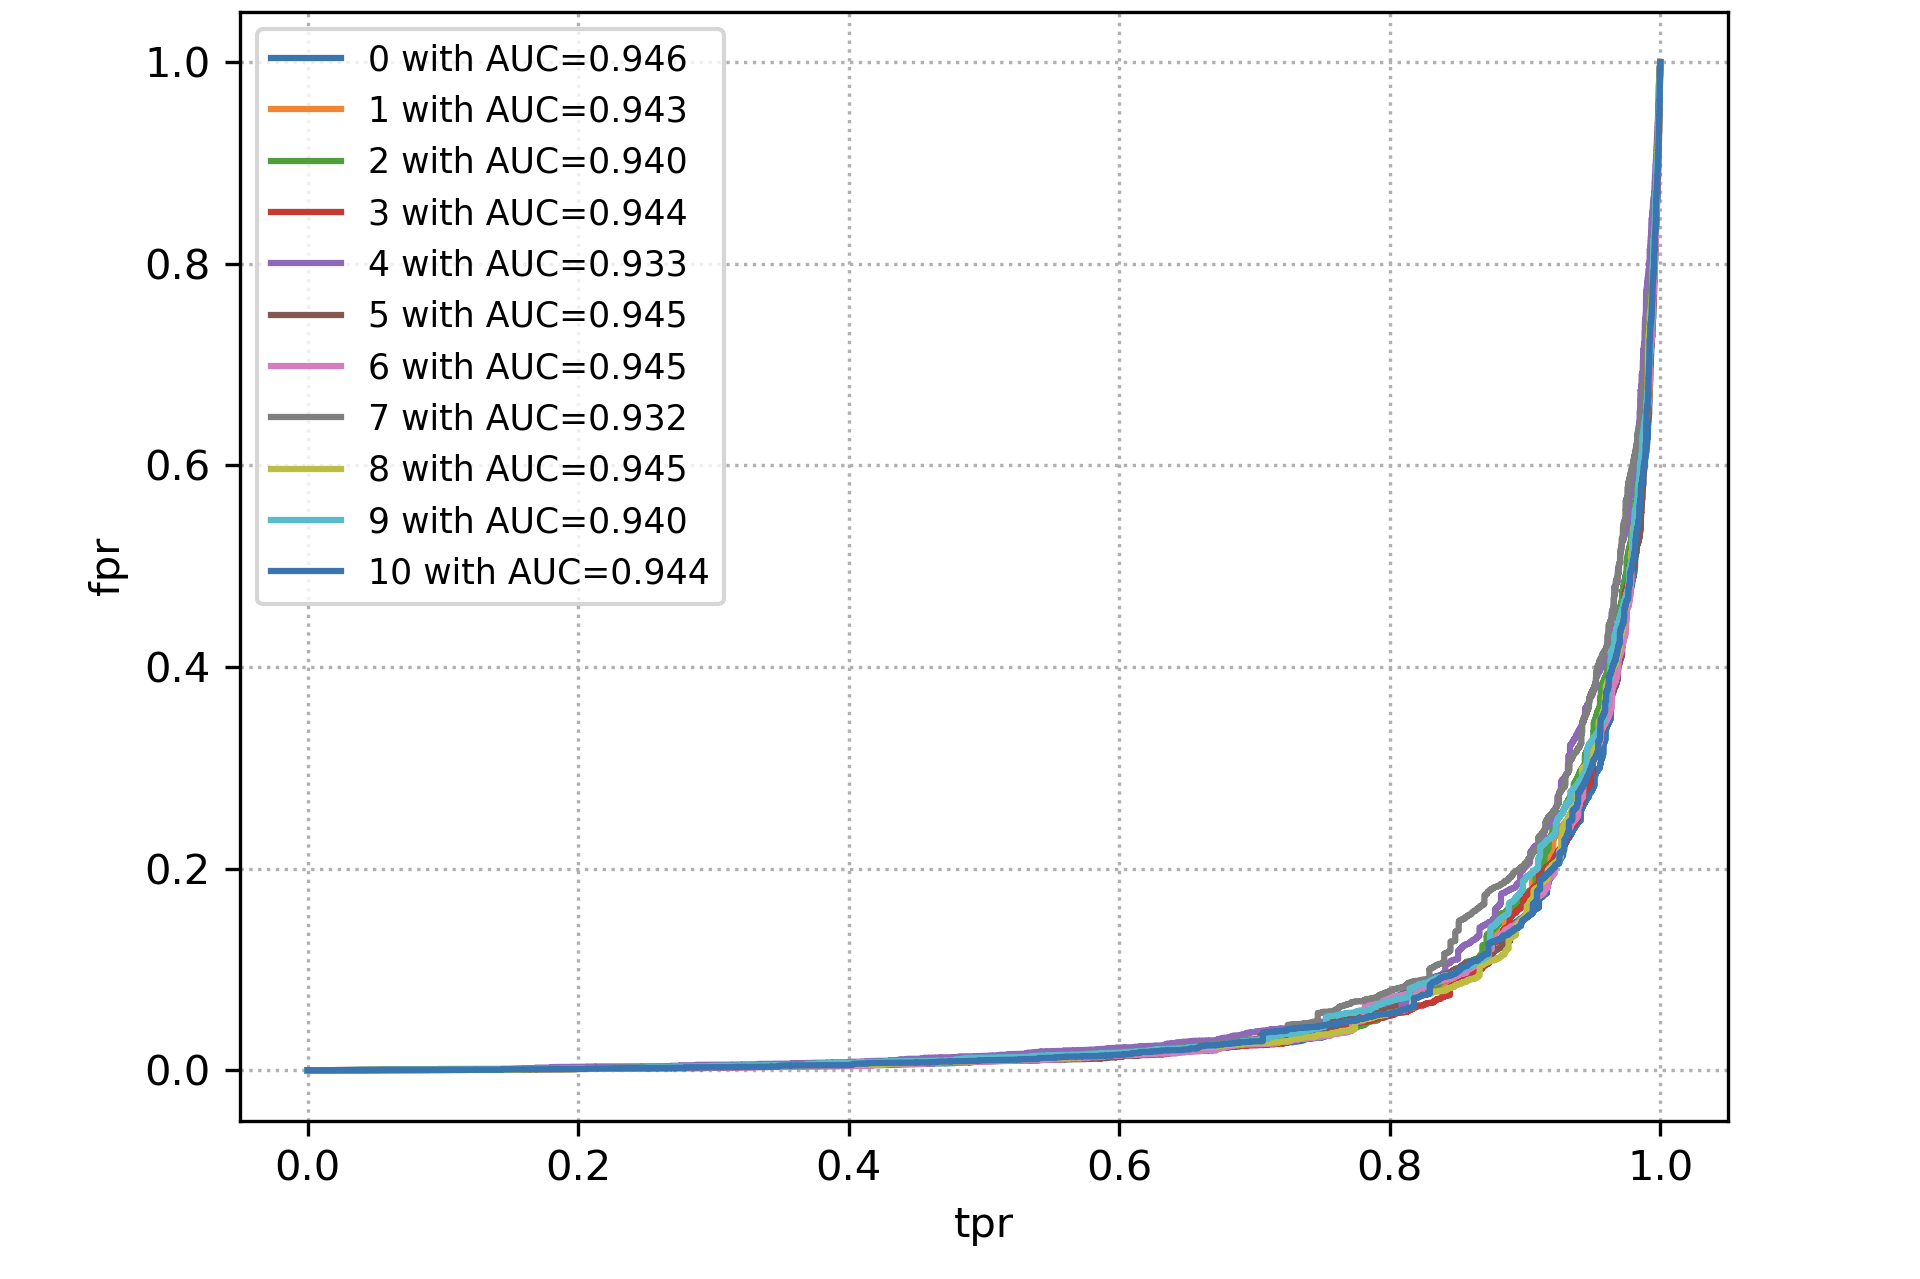
\includegraphics[width=1.1\linewidth]{Images/7.S_B/Variability/4b QCD DNN.png}
  \caption{DNN as global inputs.}
  \label{fig: 4b QCD DNN}
\end{subfigure}%
\begin{subfigure}{.5\textwidth}
  \centering
  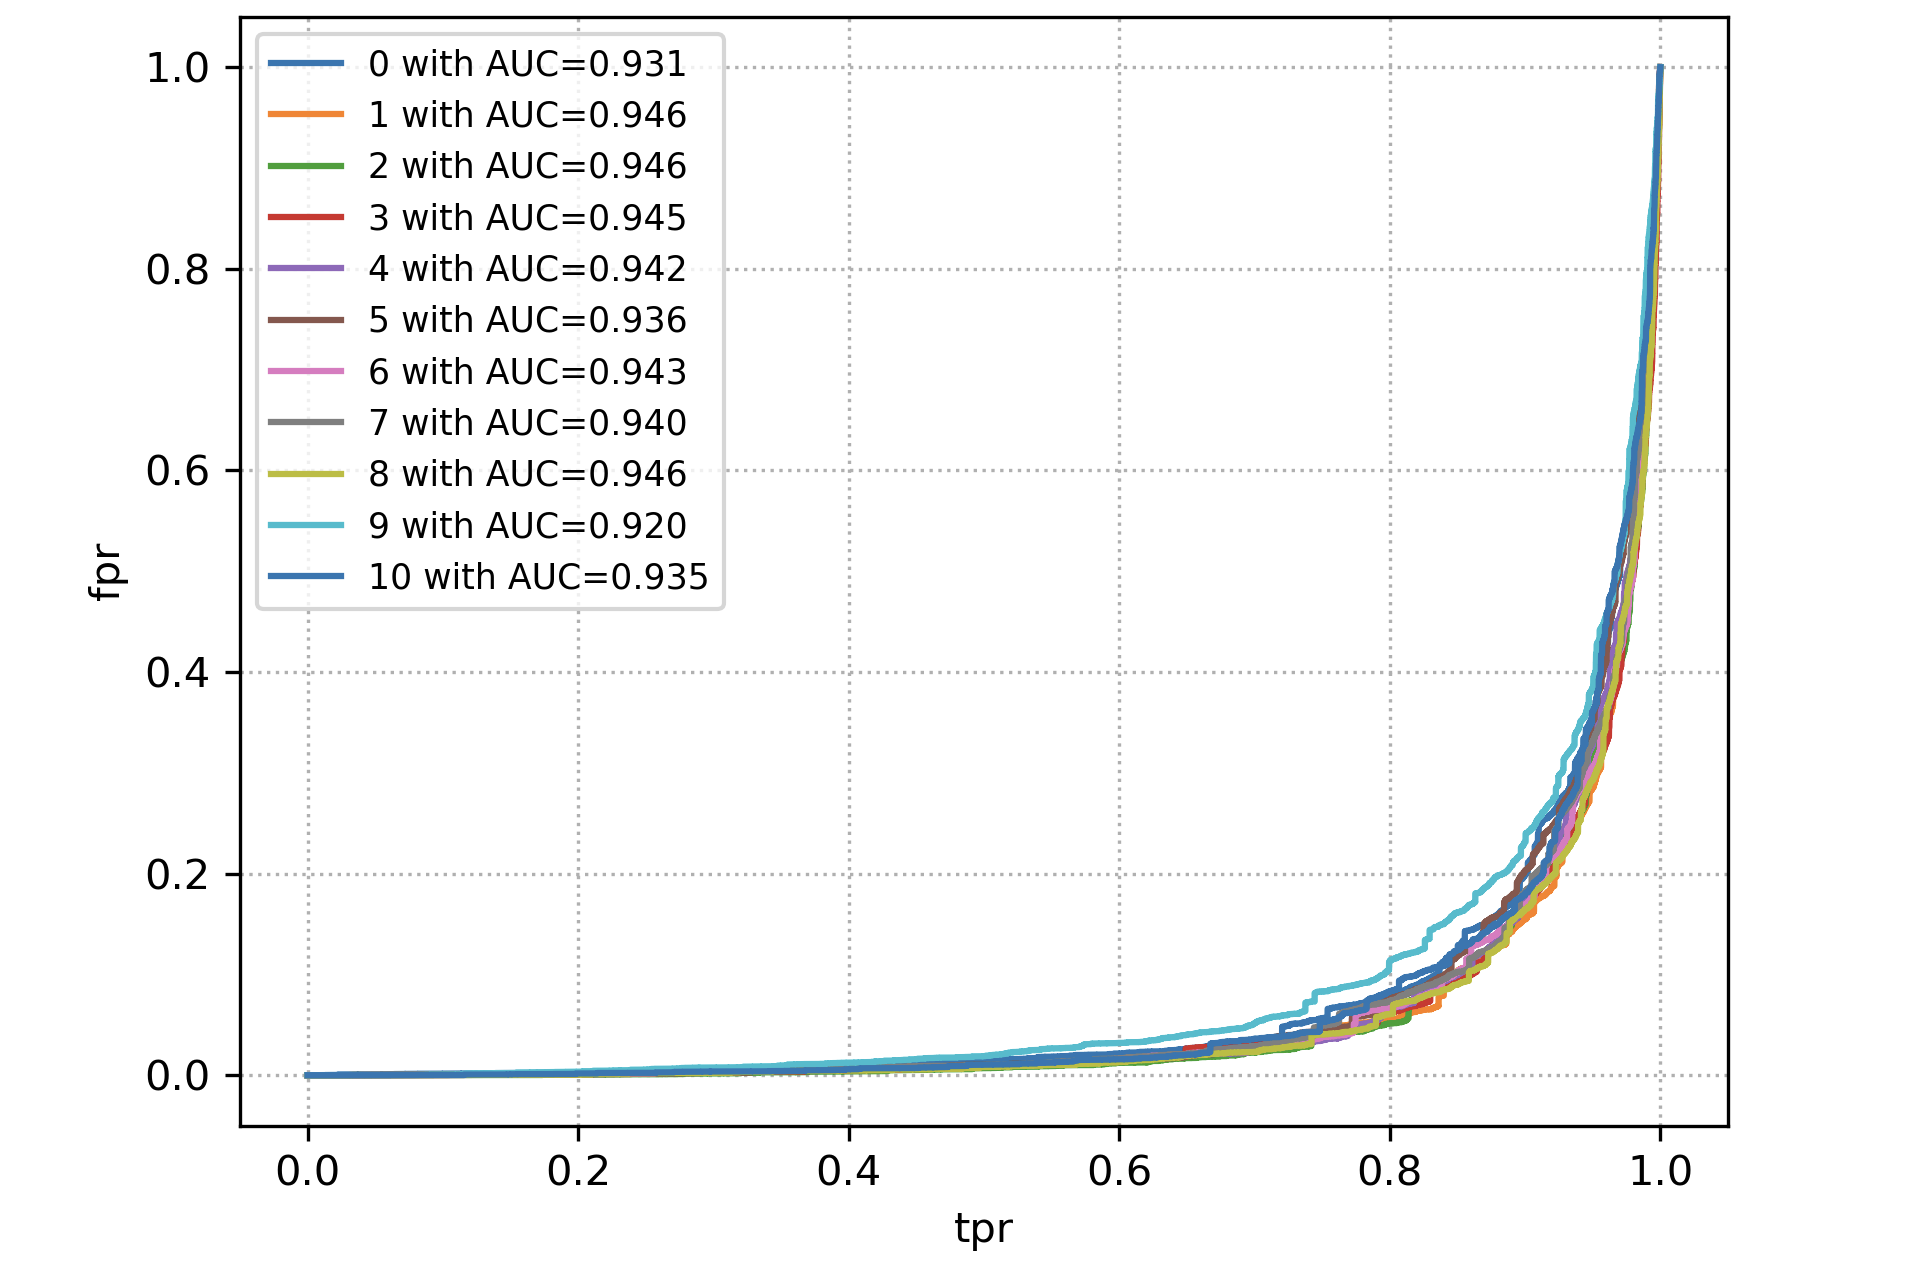
\includegraphics[width=1.1\linewidth]{Images/7.S_B/Variability/4b QCD prob diff and DNN.png}
  \caption{DNN and PD as global inputs.}
  \label{fig: 4b QCD DNN PD}
\end{subfigure}
\caption{ROC curves produced by fixing eleven different seeds using 4b-QCD and as inputs either DNN variables or DNN and PD variables. The AUC of each ROC curve are also reported in these Figures. The number next to the value of the AUC corresponds to the value of the seed fixed for the training.}
\label{fig: 4b QCD v ariability}
\end{figure}

\begin{figure}[hbt]
\centering
\begin{subfigure}{.5\textwidth}
  \centering
  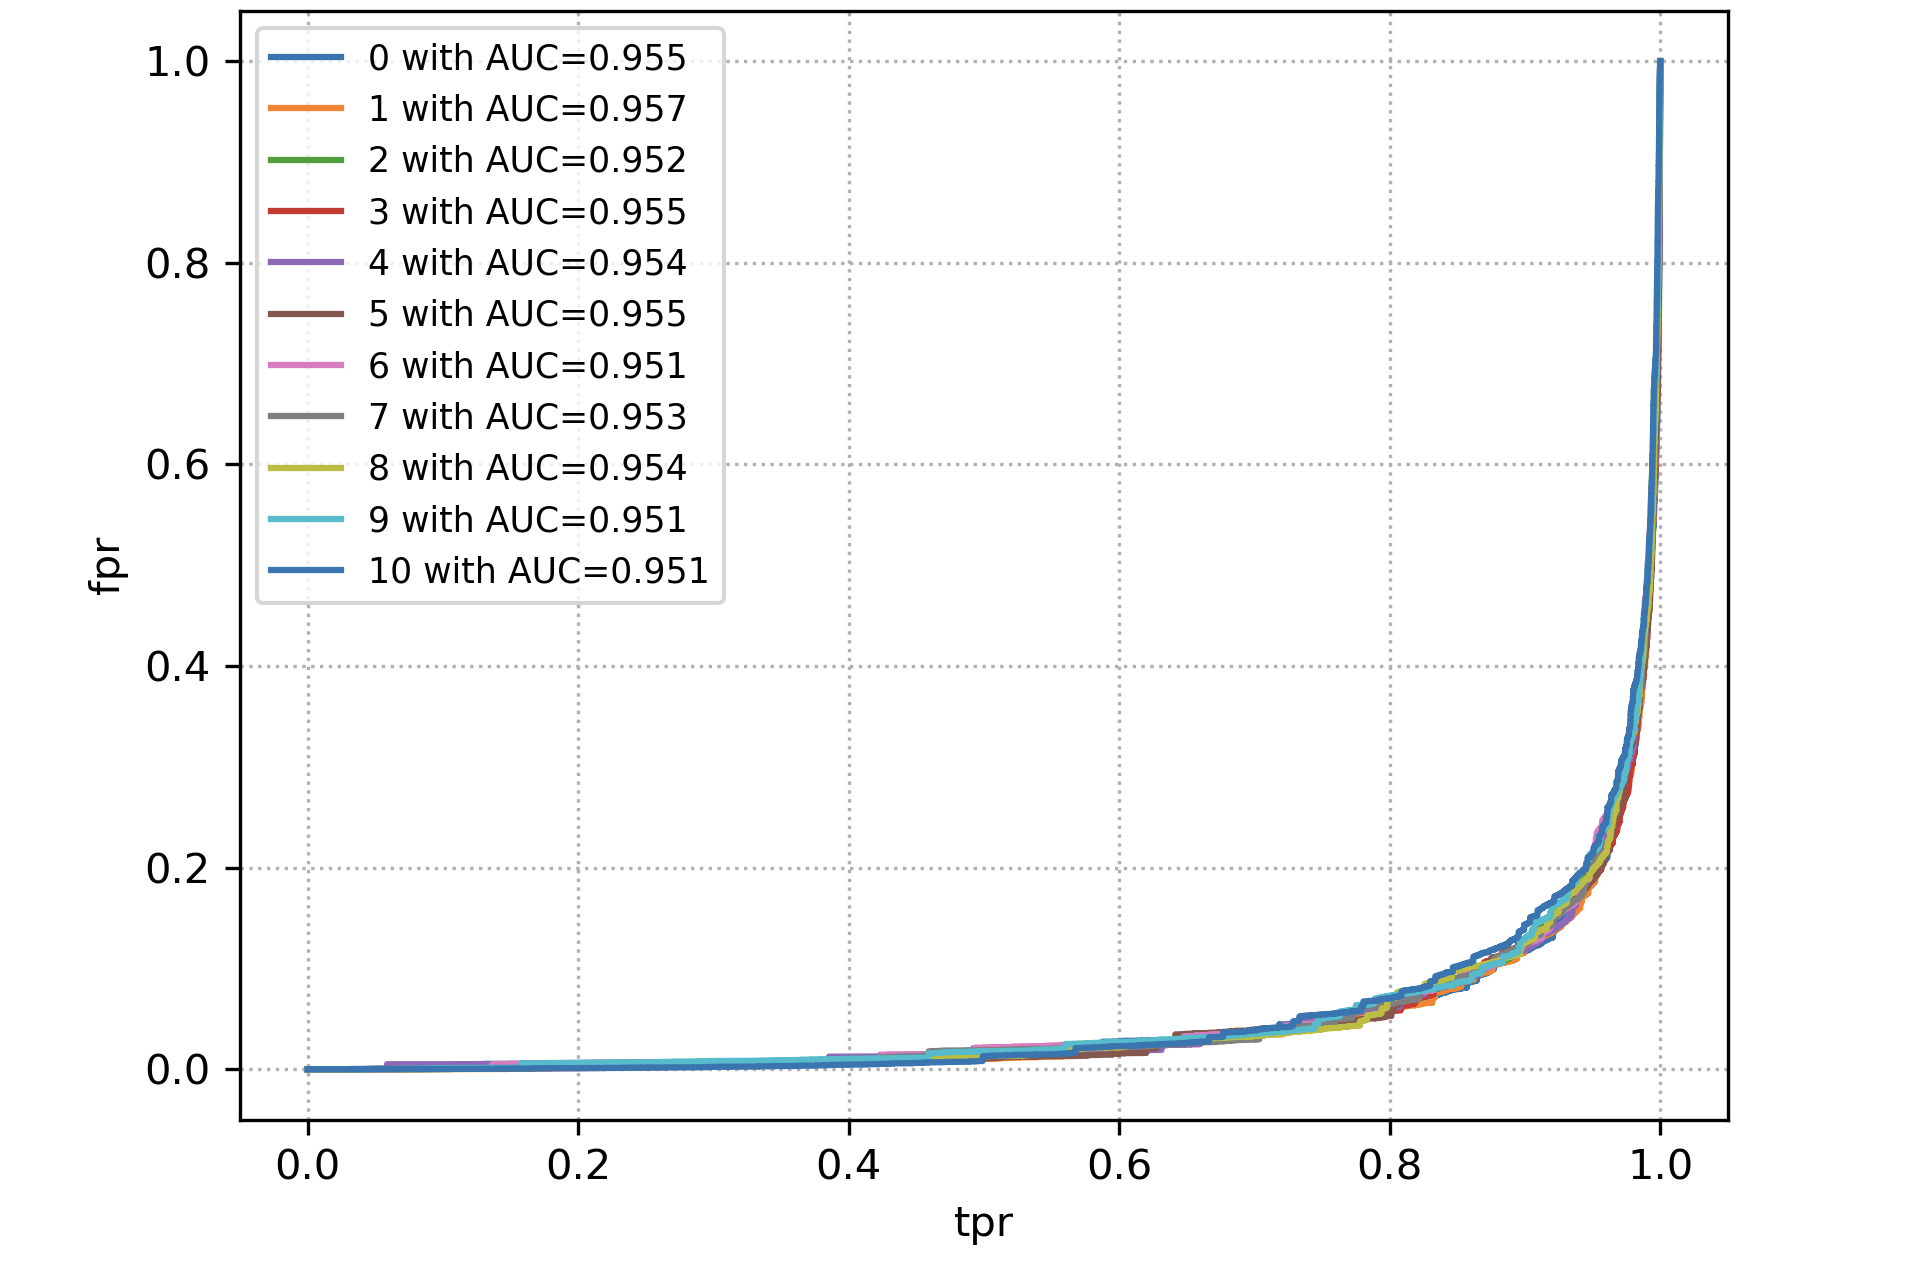
\includegraphics[width=1.1\linewidth]{Images/7.S_B/Variability/2b QCD DNN.png}
  \caption{DNN as global input}
  \label{fig: 2b QCD DNN}
\end{subfigure}%
\begin{subfigure}{.5\textwidth}
  \centering
  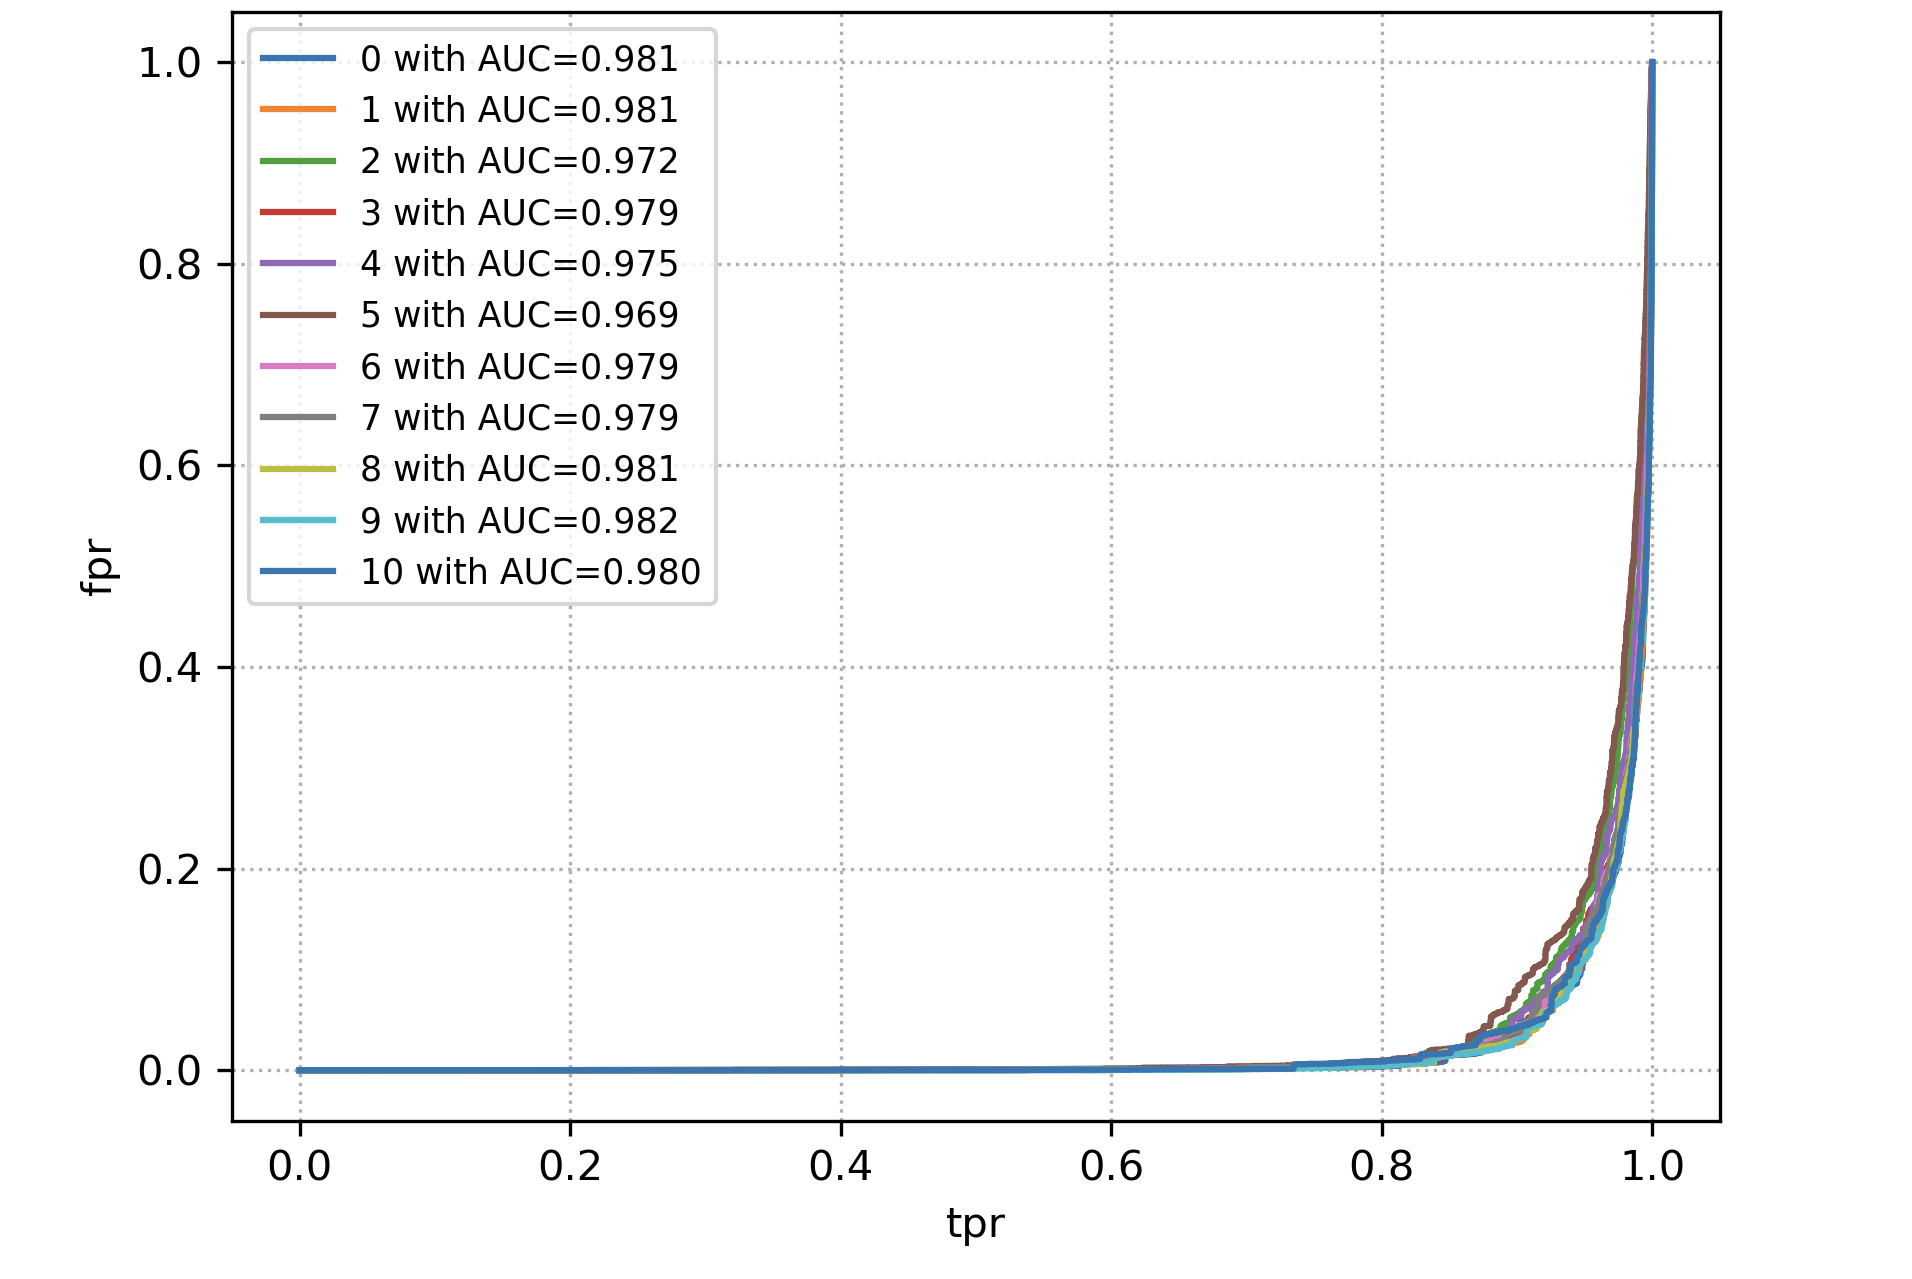
\includegraphics[width=1.1\linewidth]{Images/7.S_B/Variability/2b QCD DNN and prob diff.png}
  \caption{DNN and PD as global inputs}
  \label{fig: 2b QCD DNN PD}
\end{subfigure}
\caption{ROC curves produced by fixing eleven different seeds using 2b-QCD and as inputs either DNN variables or DNN and PD variables. The AUC of each ROC curve are also reported in these Figures. The number next to the value of the AUC corresponds to the value of the seed fixed for the training.}
\label{fig: 2b QCD v ariability}
\end{figure}

\begin{figure}[hbt]
\centering
\begin{subfigure}{.5\textwidth}
  \centering
  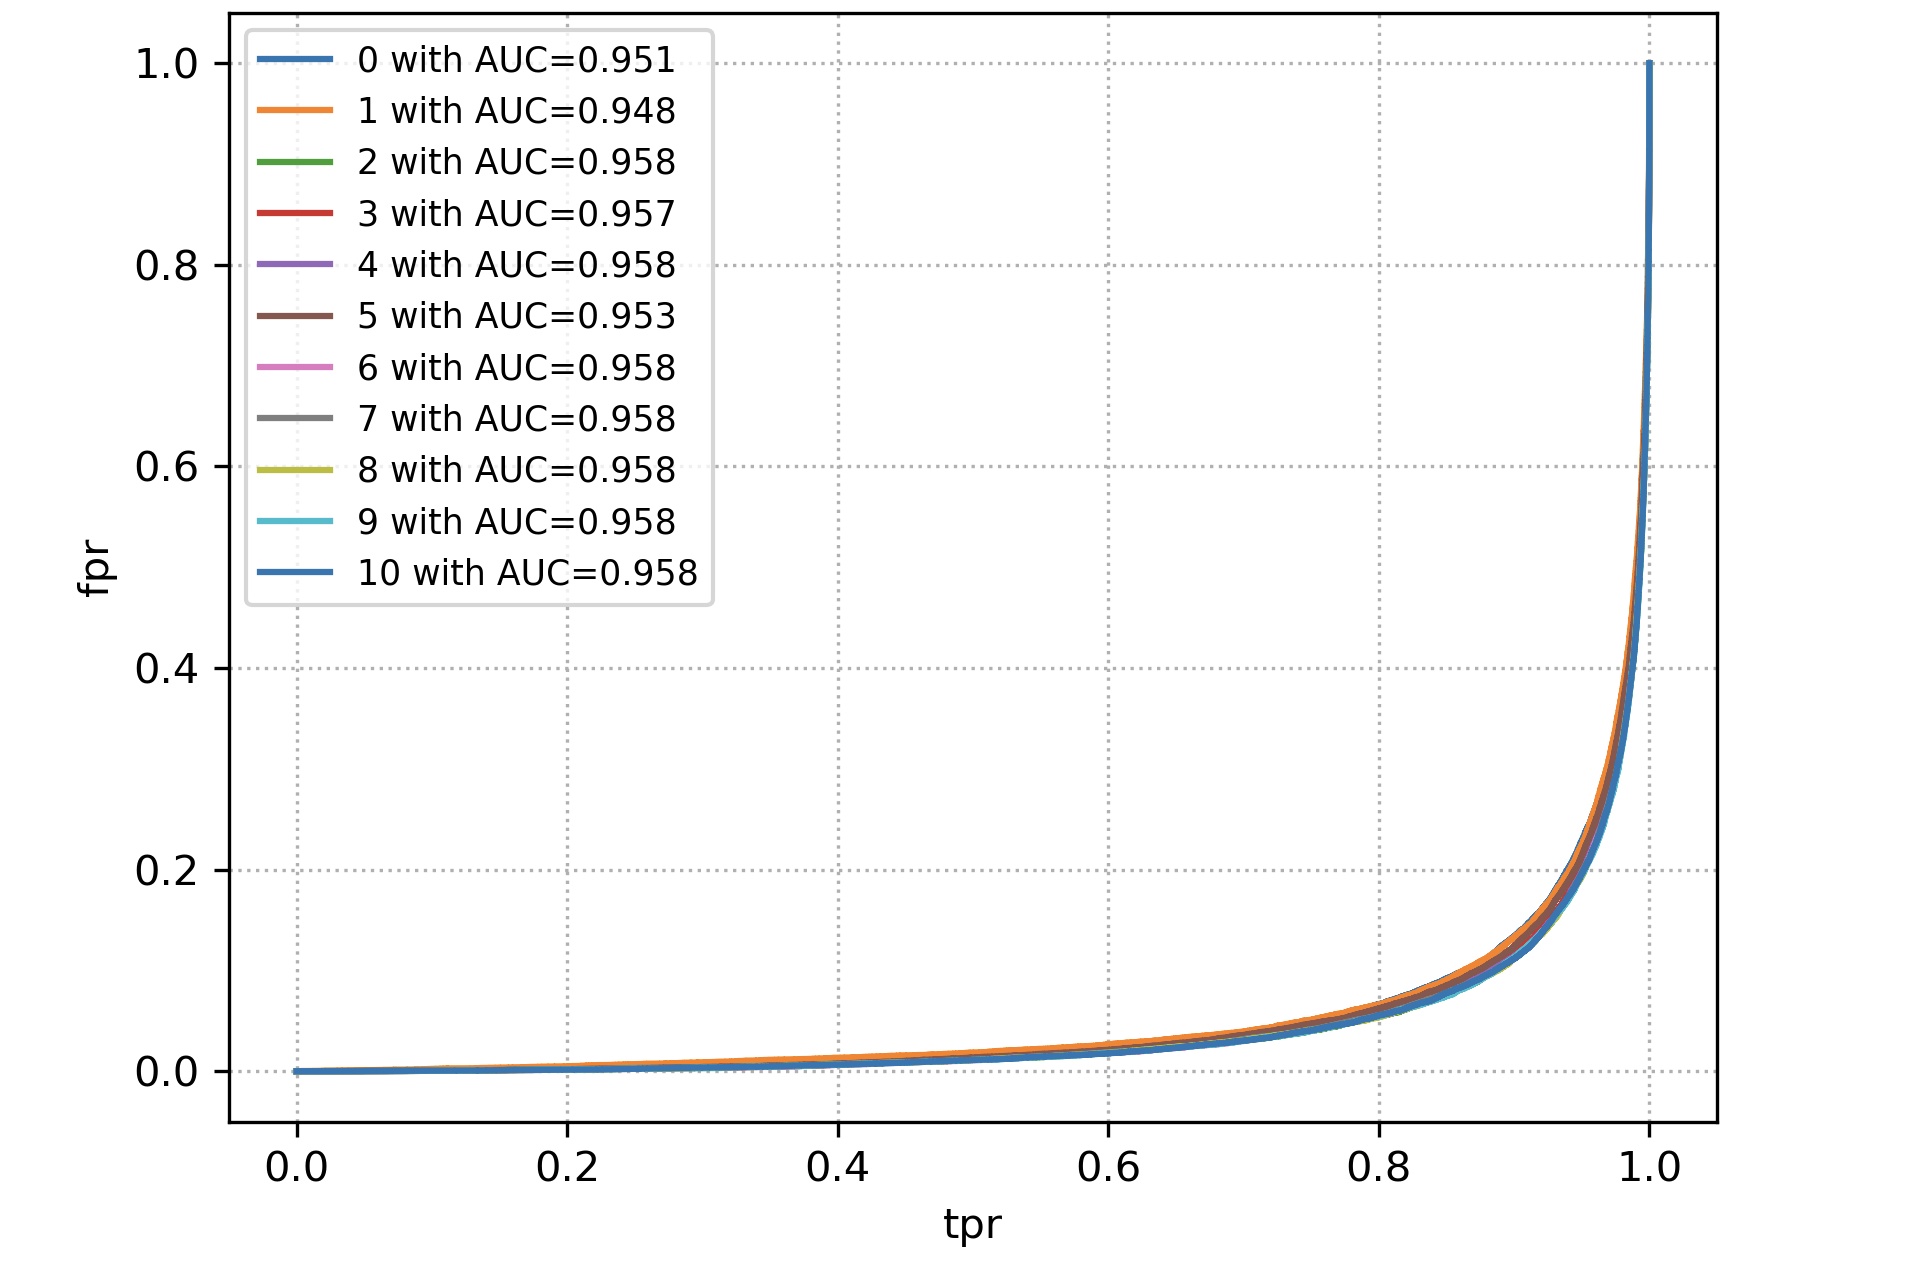
\includegraphics[width=1.1\linewidth]{Images/7.S_B/Variability/2b data DNN.png}
  \caption{DNN as global input}
  \label{fig: 2b data DNN}
\end{subfigure}%
\begin{subfigure}{.5\textwidth}
  \centering
  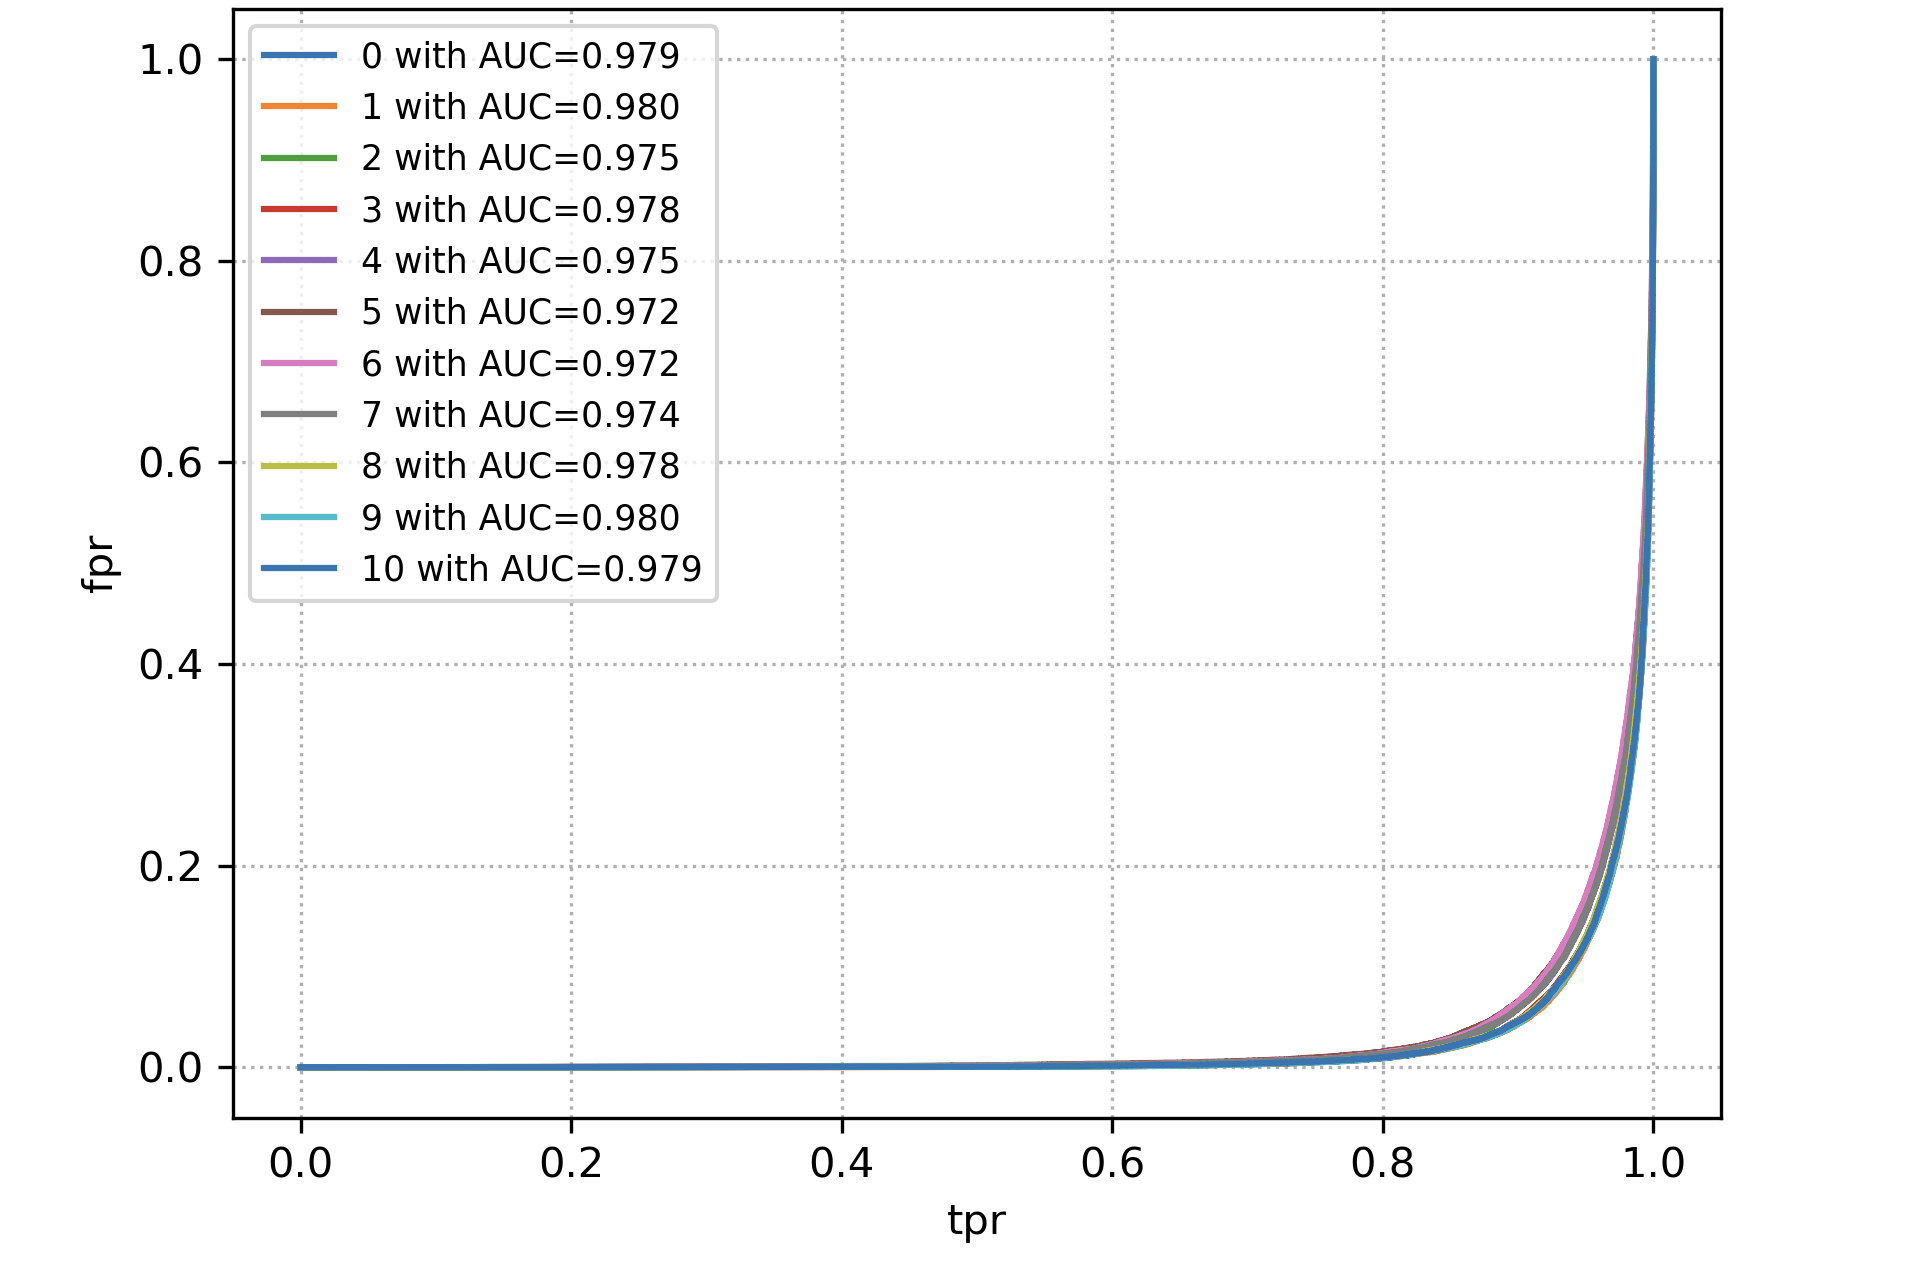
\includegraphics[width=1.1\linewidth]{Images/7.S_B/Variability/2b data DNN and prob diff.png}
  \caption{DNN and PD as global inputs}
  \label{fig: 2b data DNN PD}
\end{subfigure}
\caption{ROC curves produced by fixing eleven different seeds using 2b-data and as inputs either DNN variables or DNN and PD variables. The AUC of each ROC curve is also reported in these Figures. The number next to the value of the AUC corresponds to the value of the seed fixed for the training.}
\label{fig: 2b data v ariability}
\end{figure}

\begin{table}[hbt]
\centering
\begin{tabular}{|M{5cm}||M{2.5cm}|M{2.5cm}|M{2.5cm}|}
 \hline
 Configuration  & Maximum value of the AUC & Minimum value of the AUC & Variability \\
 \hline
 \hline
 4b-QCD (DNN) & 0.949 & 0.932 & $\sim$0.017 \\
 \hline
 4b-QCD (DNN and PD) & 0.946 & 0.920 & $\sim$0.026 \\
 \hline
 \hline
 2b-QCD (DNN) & 0.957 & 0.951 & $\sim$0.008\\
 \hline
 2b-QCD (DNN and PD) & 0.982 & 0.969 & $\sim$0.013 \\
 \hline
 \hline
 2b-data (DNN) & 0.958 & 0.948 & $\sim$0.01 \\
 \hline
 2b-data (DNN and PD) & 0.980 & 0.972 & $\sim$0.008  \\
 \hline
\end{tabular}
\caption{Maximal and minimal AUC values observed in Figures \ref{fig: 4b QCD v ariability}, \ref{fig: 2b QCD v ariability}, \ref{fig: 2b data v ariability} and  variability of the 4b-QCD, 2b-QCD and 2b data configurations.}
\label{table: Spread of the trainings}
\end{table}


Due to some limitations in our available resources, we could not compute the variability for 2b data full statistics, nevertheless, we observed that the value of the AUC was not affected (within the variability of the training) by the difference in statistics, as shown in Table \ref{table: 2b-data AUC r vs f}.


\begin{table}[hbt]
\centering
\begin{tabular}{|M{7cm}|M{4cm}|}
 \hline
 Configuration  & Value of the AUC \\
 \hline
 \hline
 2b-data reduced statistics (DNN) & 0.951  \\
 \hline
 2b-data full statistics (DNN) & 0.958 \\
\hline
 \hline
 2b-data reduced statistics (DNN and PD) & 0.979 \\
 \hline
 2b-data full statistics (DNN and PD) & 0.977  \\
\hline
\end{tabular}
\caption{Results of the AUC obtained after training SPANet on 2b-data full and reduced statistics.}
\label{table: 2b-data AUC r vs f}
\end{table}


\subsection{Inference of the 4b data ROC} \label{subsection:4b data extrapolation inclusivce}

In the previous Sections the necessary inputs to infer the 4b data AUC and ROC curve using Eq.(\ref{eq: extrapolation}) are presented. Since there is not an immediate solution to reduce the variability on the 4b-QCD trainings, as a first approximation for the inference, the b-tag ratio in Eq.(\ref{eq: extrapolation}) is computed for the 11 seeds and check where the value from the AN used for the comparison lies within this variability. Since the variability for 2b-QCD and 2b-data is small ($\sim 0.01$), it has been decided to ignore this variability to infer the 4b-data results.

Figures \ref{fig: 4b data extrapolation DNN} and \ref{fig: 4b data extrapolation DNN PD} show the results of the ROC inferred for 4b data and the comparison to the ROC in the AN. The values of the AUC reported in these plots are the extrapolated values computed using Eq.(\ref{eq: extrapolation}). These plots show the best and the worst performing ROC curves in terms of variability of the SPANet training to compare with more clarity where the AN ROC, the benchmark ROC the comparison is done against, lies within the variability of these trainings. We conclude that using the PD variable does not improve the SPANet performance. For both cases, the results from the AN are within the variability of our trainings. 

\begin{figure}[hbt]
    \centering
    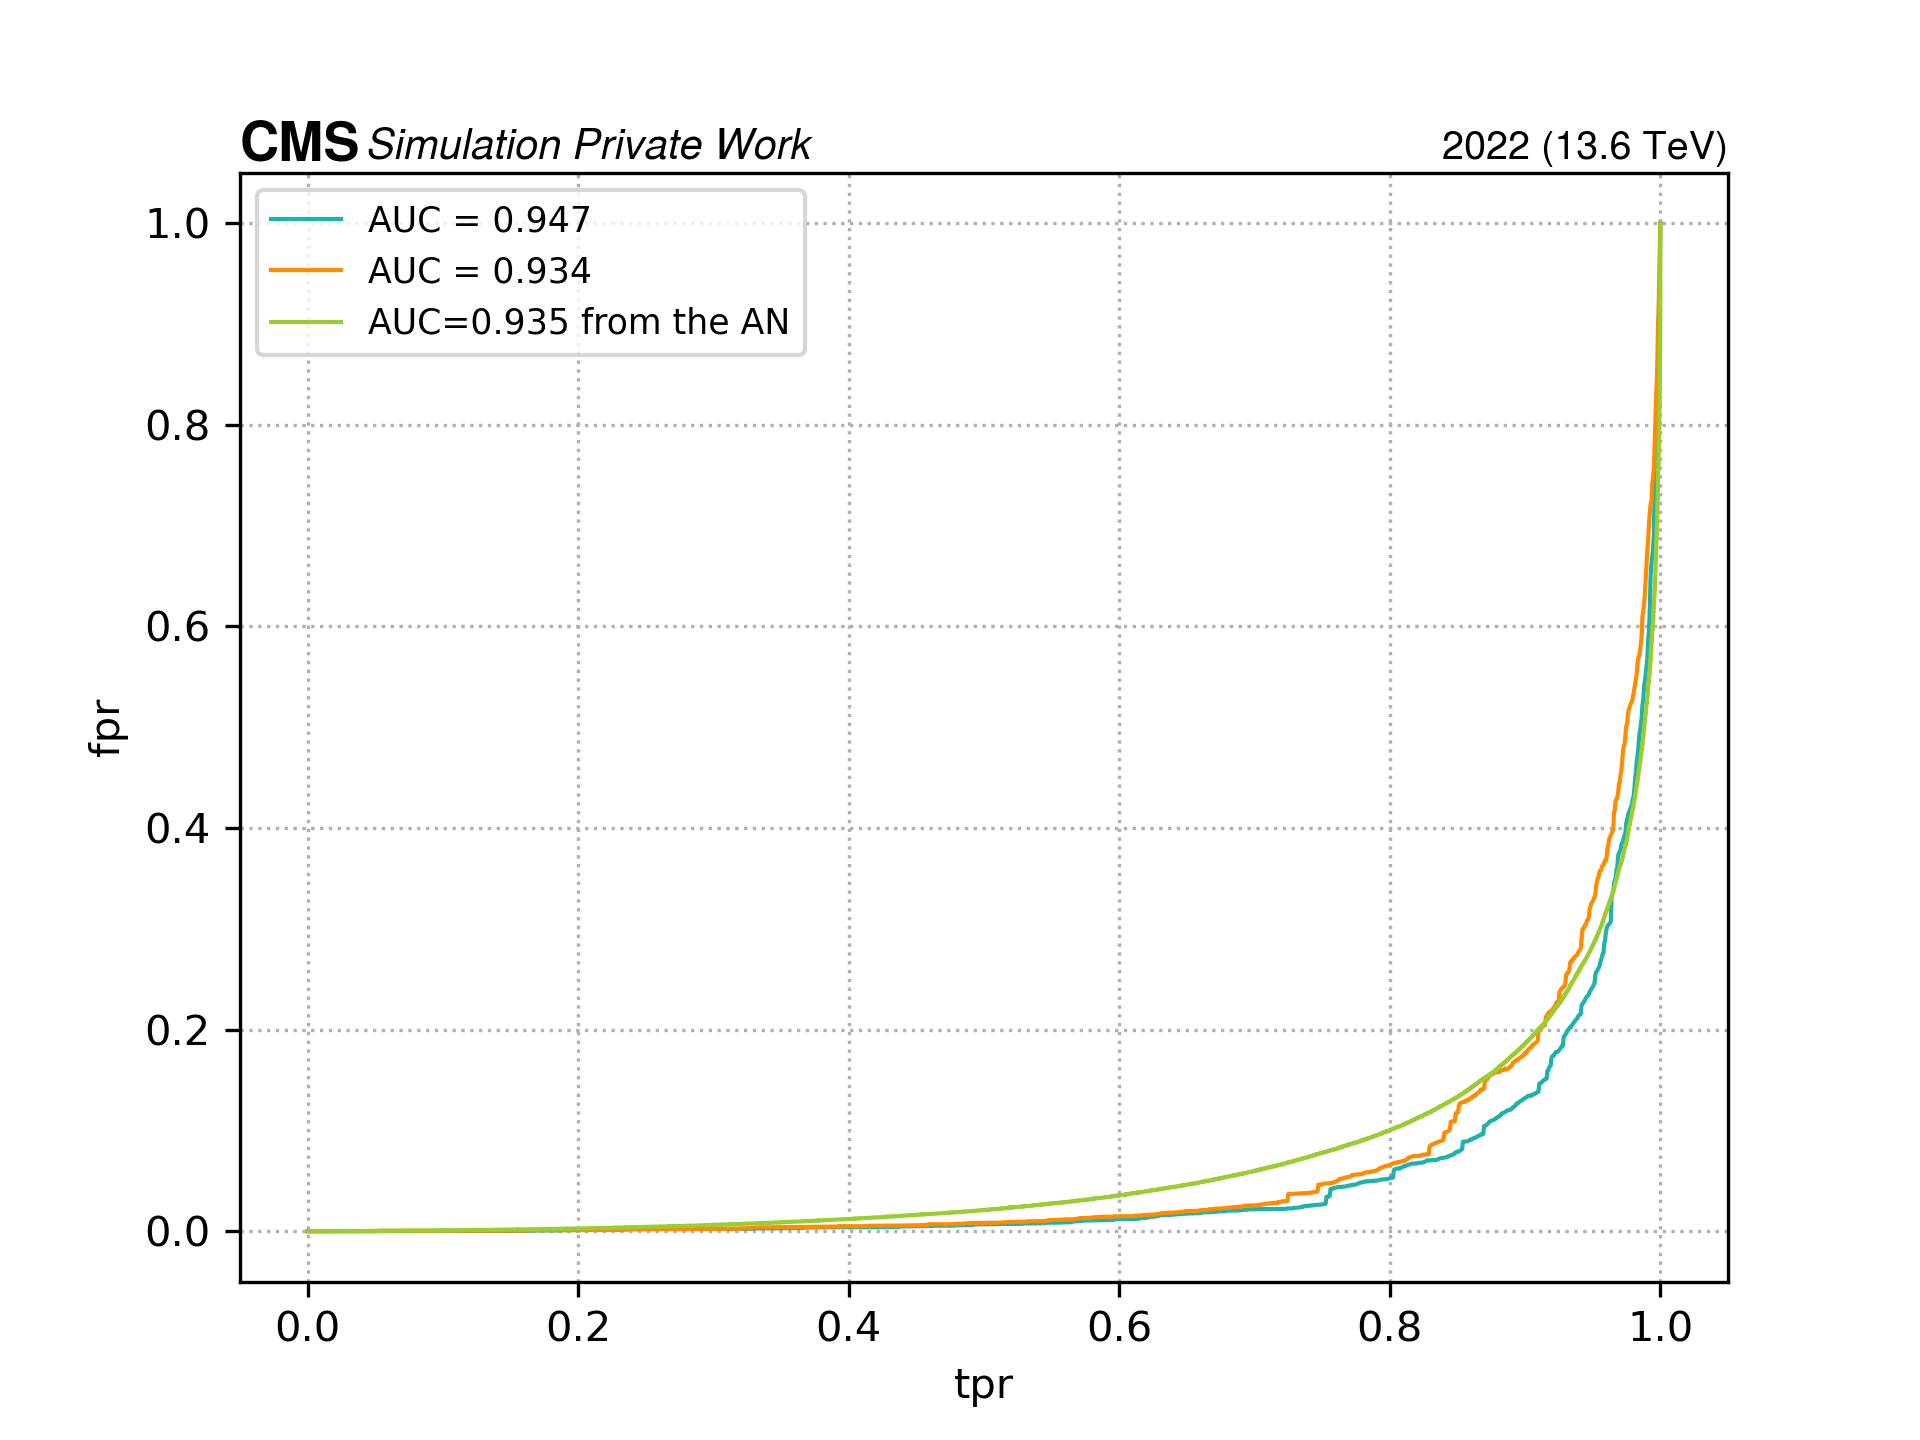
\includegraphics[width=0.7\linewidth]{Images/7.S:B/Extrapolation/4b data dnn.png}
    \caption{ROC curve inferred for 4b-data, with DNN as inputs, using Eq.(\ref{eq: extrapolation}) to compute the FPR and the TPR is taken from 2b data full statistics ROC curve. The AUCs showed in this Figure are the inferred using Eq.(\ref{eq: extrapolation})}
    \label{fig: 4b data extrapolation DNN}
\end{figure}

\begin{figure}[hbt]
    \centering
    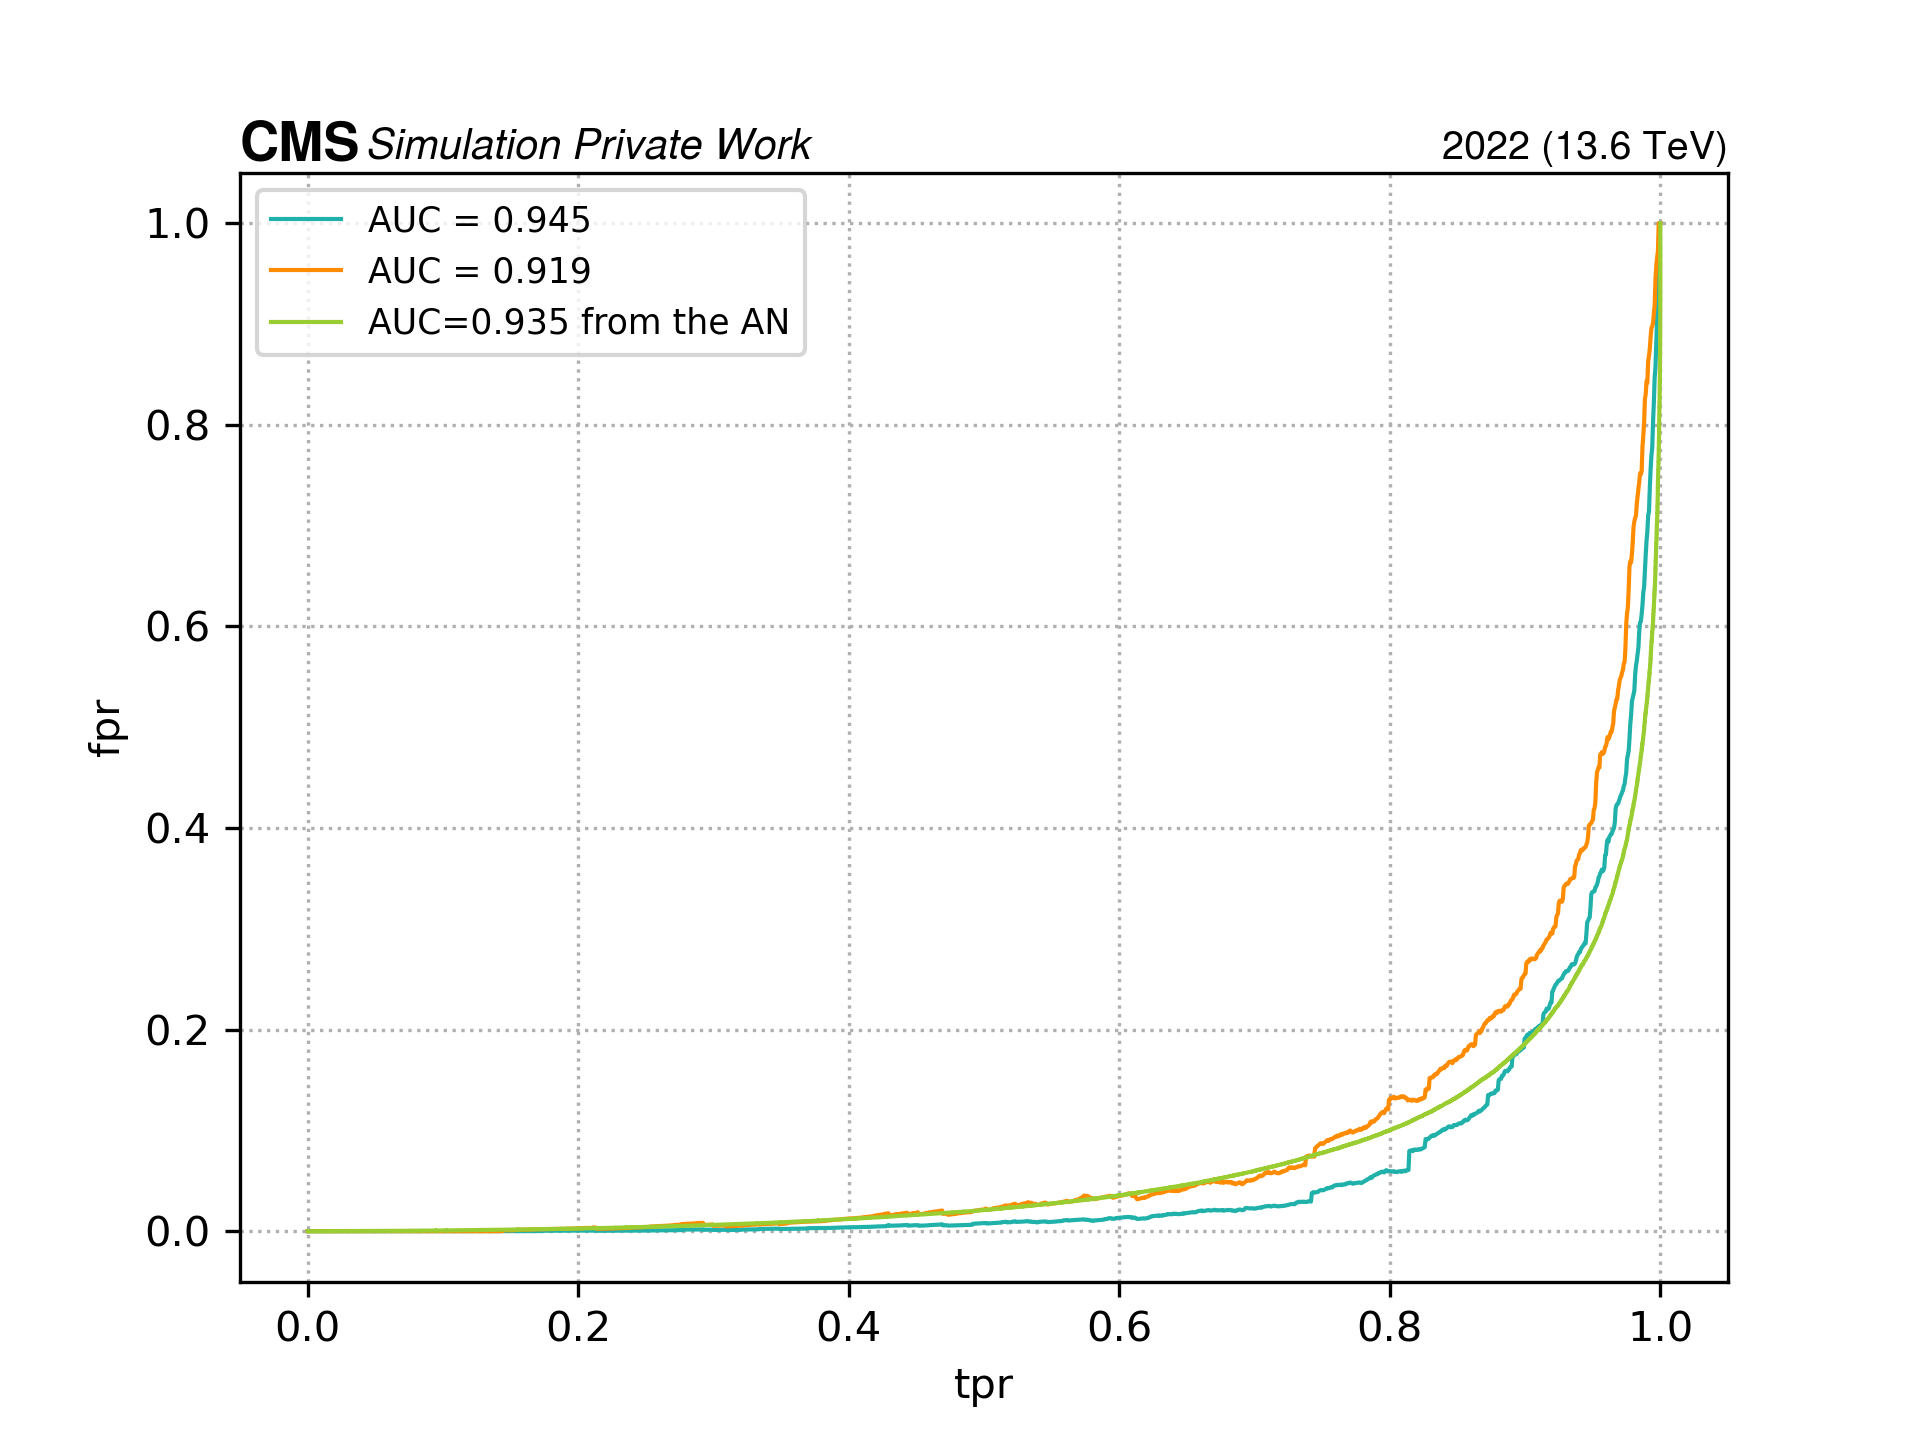
\includegraphics[width=0.7\linewidth]{Images/7.S:B/Extrapolation/4b data dnn proba.png}
    \caption{ROC curve inferred for 4b-data, with DNN and PD as inputs, using Eq.(\ref{eq: extrapolation}) to compute the FPR and the TPR is taken from 2b data full statistics ROC curve. The AUCs showed in this Figure are the inferred using Eq.(\ref{eq: extrapolation}).}
    \label{fig: 4b data extrapolation DNN PD}
\end{figure}


\clearpage

\subsection{Signal region}

So far the training of the SPANet models has been done inclusively in the analysis phase-space and the results have been compared to the results in the AN. Nevertheless, the results in the AN have been obtained by training the DNN with samples considering only events in the analysis SR (defined in Section \ref{section: HH4b}). Therefore, the inclusive SPANET model will be first evaluated in the SR, and afterwards dedicated training and evaluations of the SPANET model will be performed in the SR.


\subsubsection{Evaluation of the SPANET model in the SR}

The evaluation of the inclusive trainings on SR samples was tested. Figure \ref{fig: 2b data comparison ev on SR} shows the comparison between the evaluation of the SPANet 2b-data full statistics inclusive training on the 2b-data full statistics sample in the SR and on the 2b-data full statistics inclusive sample. It is to observe that the training using DNN and PD as global variables has the same performance when evaluating on SR or inclusively within the variability. Nevertheless, for 2b-data using only DNN as inputs a significant loss in performance is observed.

\begin{figure}[hbt]
    \centering
    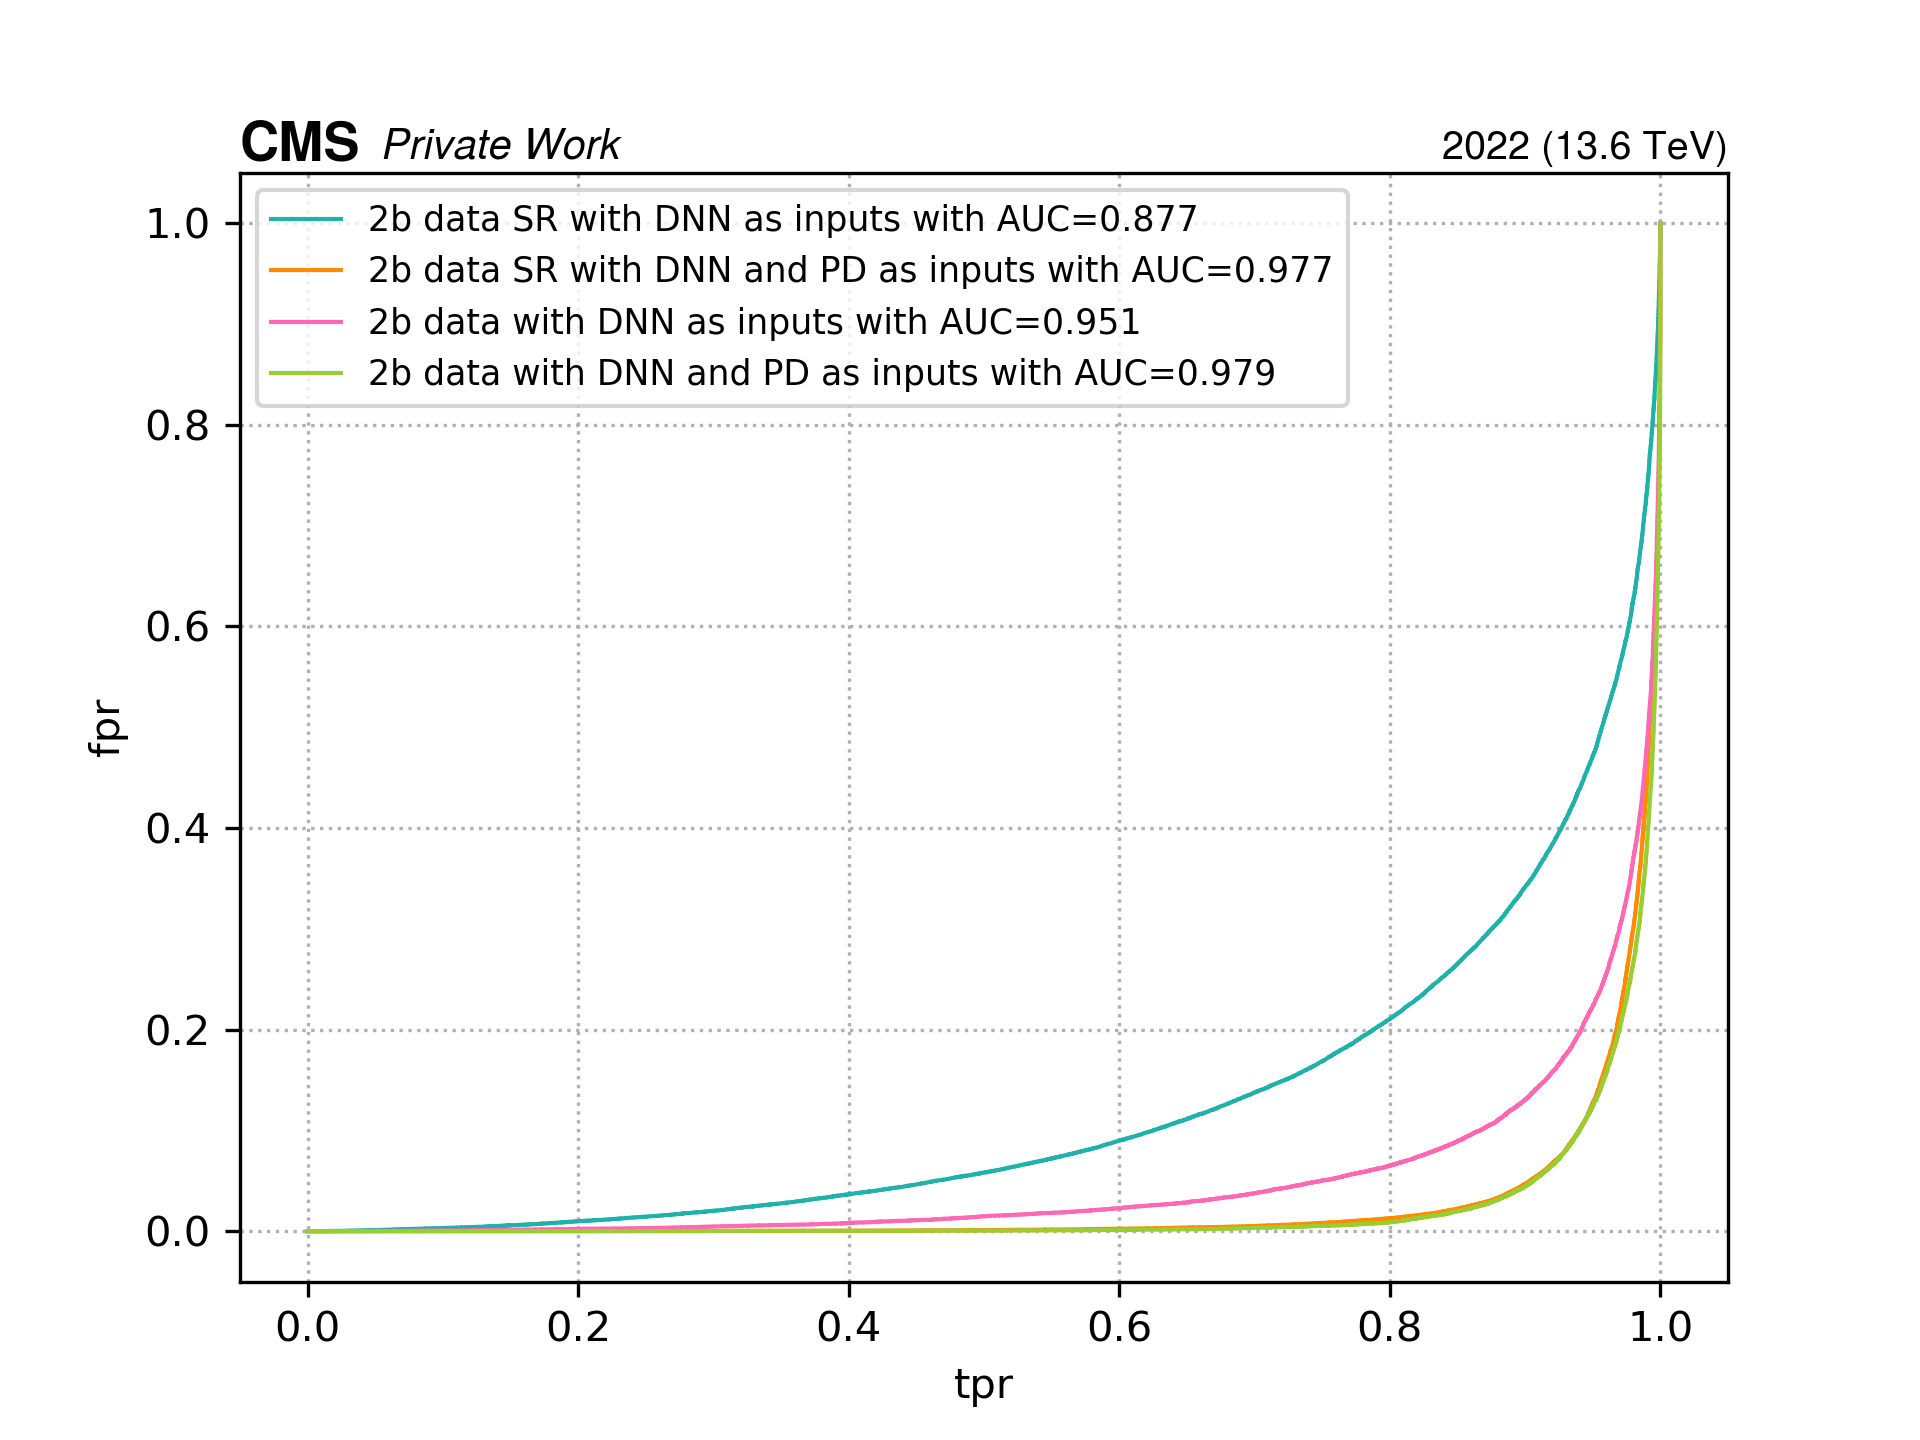
\includegraphics[width=0.7\linewidth]{Images/7.S:B/SR stats/2b-data comp.png}
    \caption{ROC curves of the SPANet 2b-data full statistics inclusive trainings using DNN or PD and DNN as input variables evaluated inclusively and in the SR. The samples named 2b data SR are the ones containing only events in the SR.}
    \label{fig: 2b data comparison ev on SR}
\end{figure}

Moreover Figures \ref{fig: ev on SR dnn} and \ref{fig: ev on SR dnn pd}, show the the ROC curve inferred for 4b-data when evaluating on SR samples. It is observed that the SPANet classification performance worsens significantly due to the fact that the SPANet training is performed inclusively and applied in the SR. Therefore, a dedicated training in the SR will be discussed in the next Section.

\begin{figure}[hbt]
    \centering
    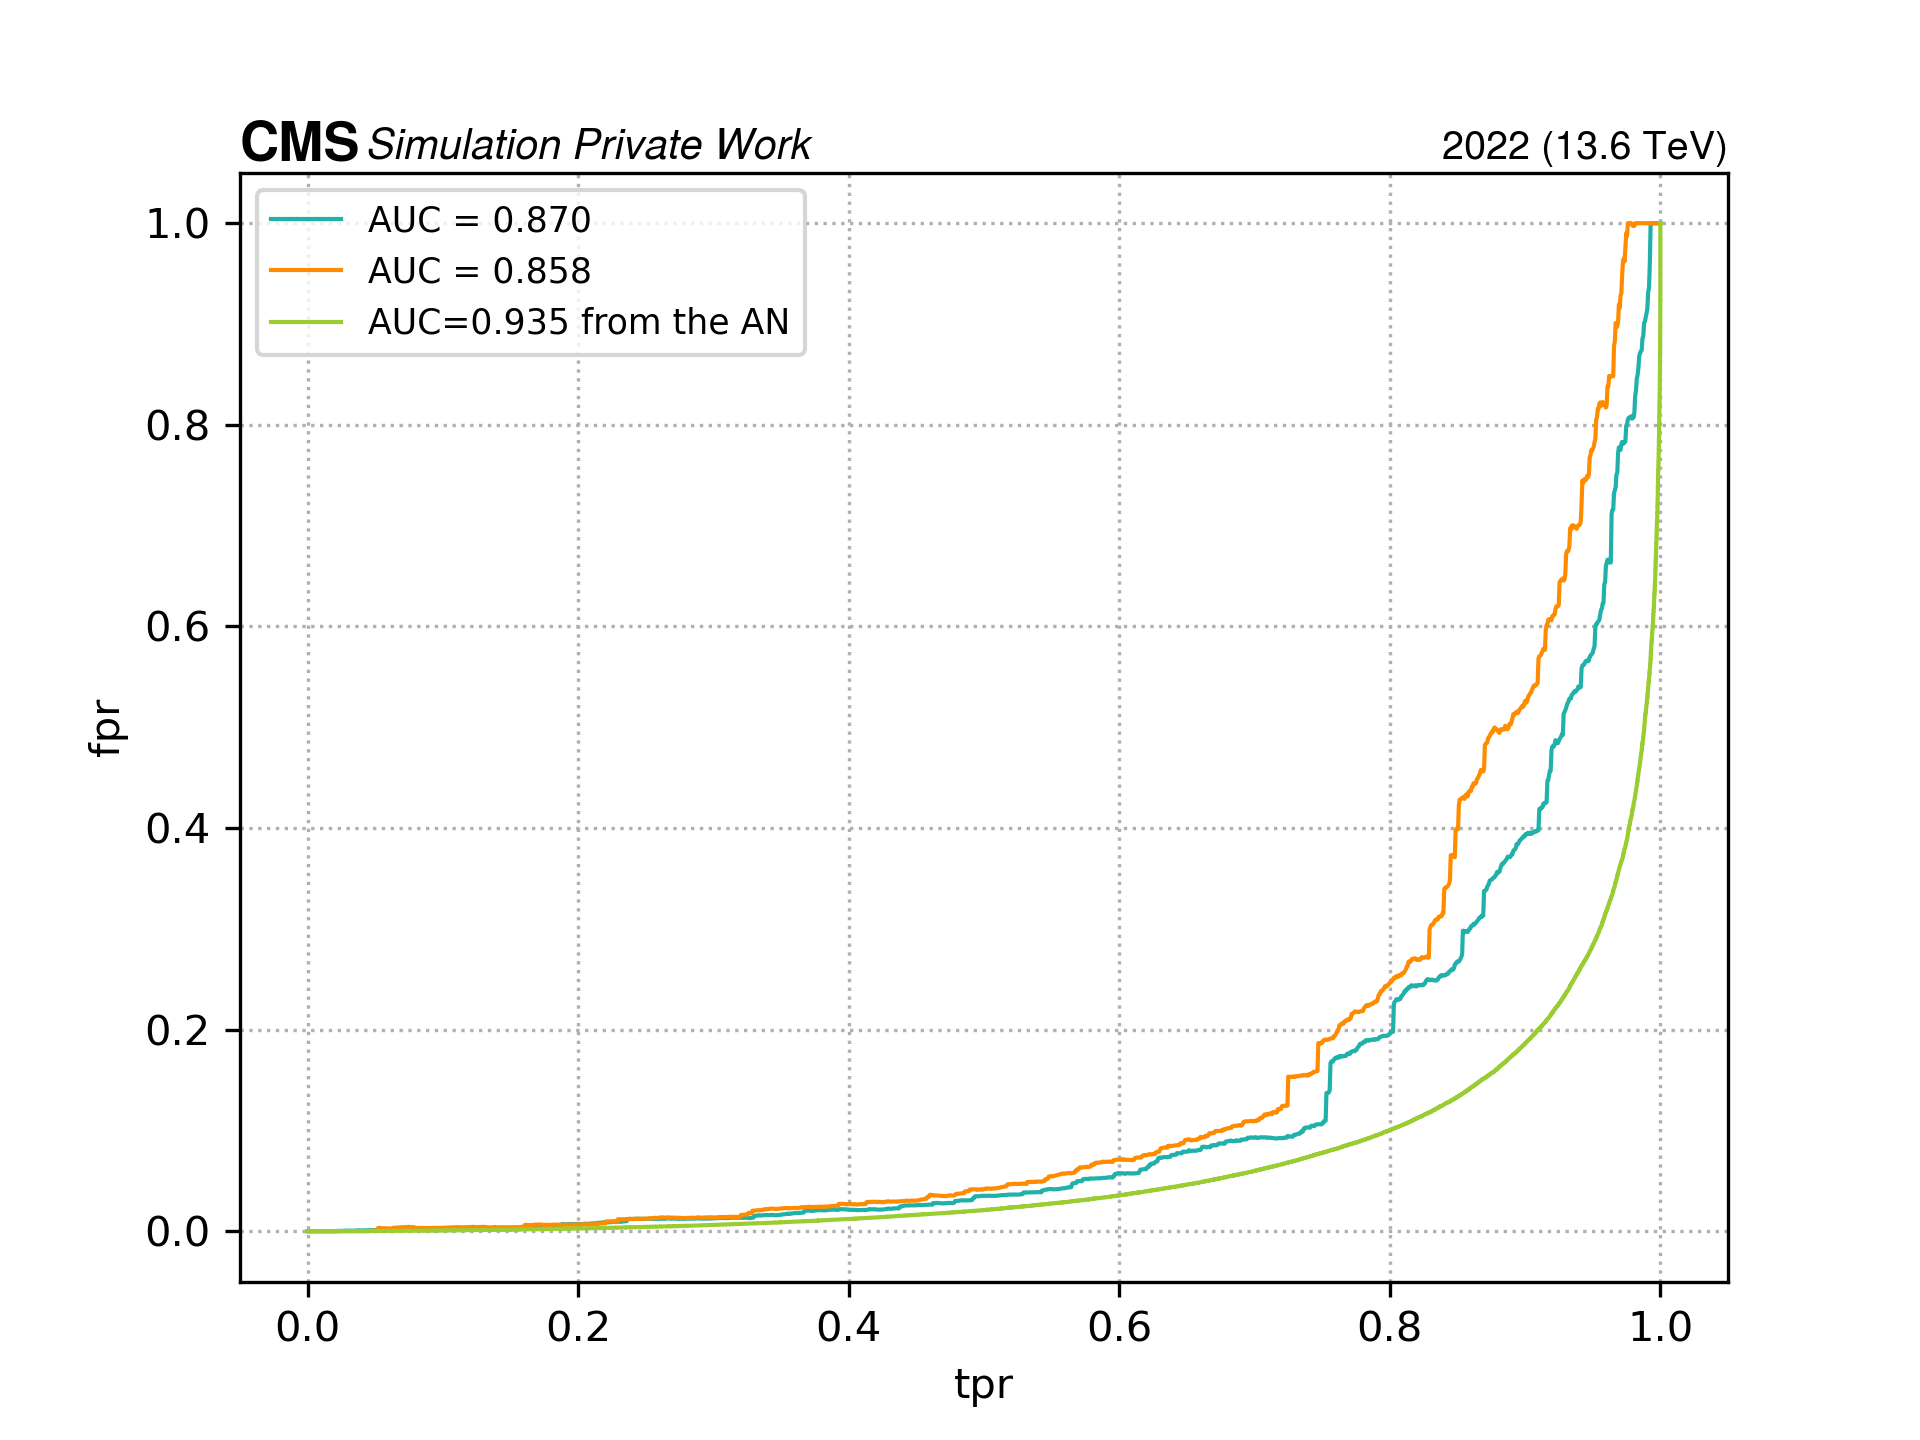
\includegraphics[width=0.7\linewidth]{Images/7.S:B/SR stats/4b data extrapol ev on SR dnn.png}
    \caption{ROC curve inferred for 4b-data using the inclusive trainings with DNN as inputs to compute FPR using Eq.(\ref{eq: extrapolation}). The TPR values are taken from the 2b data full statistics ROC curve. The AUCs showed in this Figure are inferred using Eq.(\ref{eq: extrapolation}).}
    \label{fig: ev on SR dnn}
\end{figure}

\begin{figure}[hbt]
    \centering
    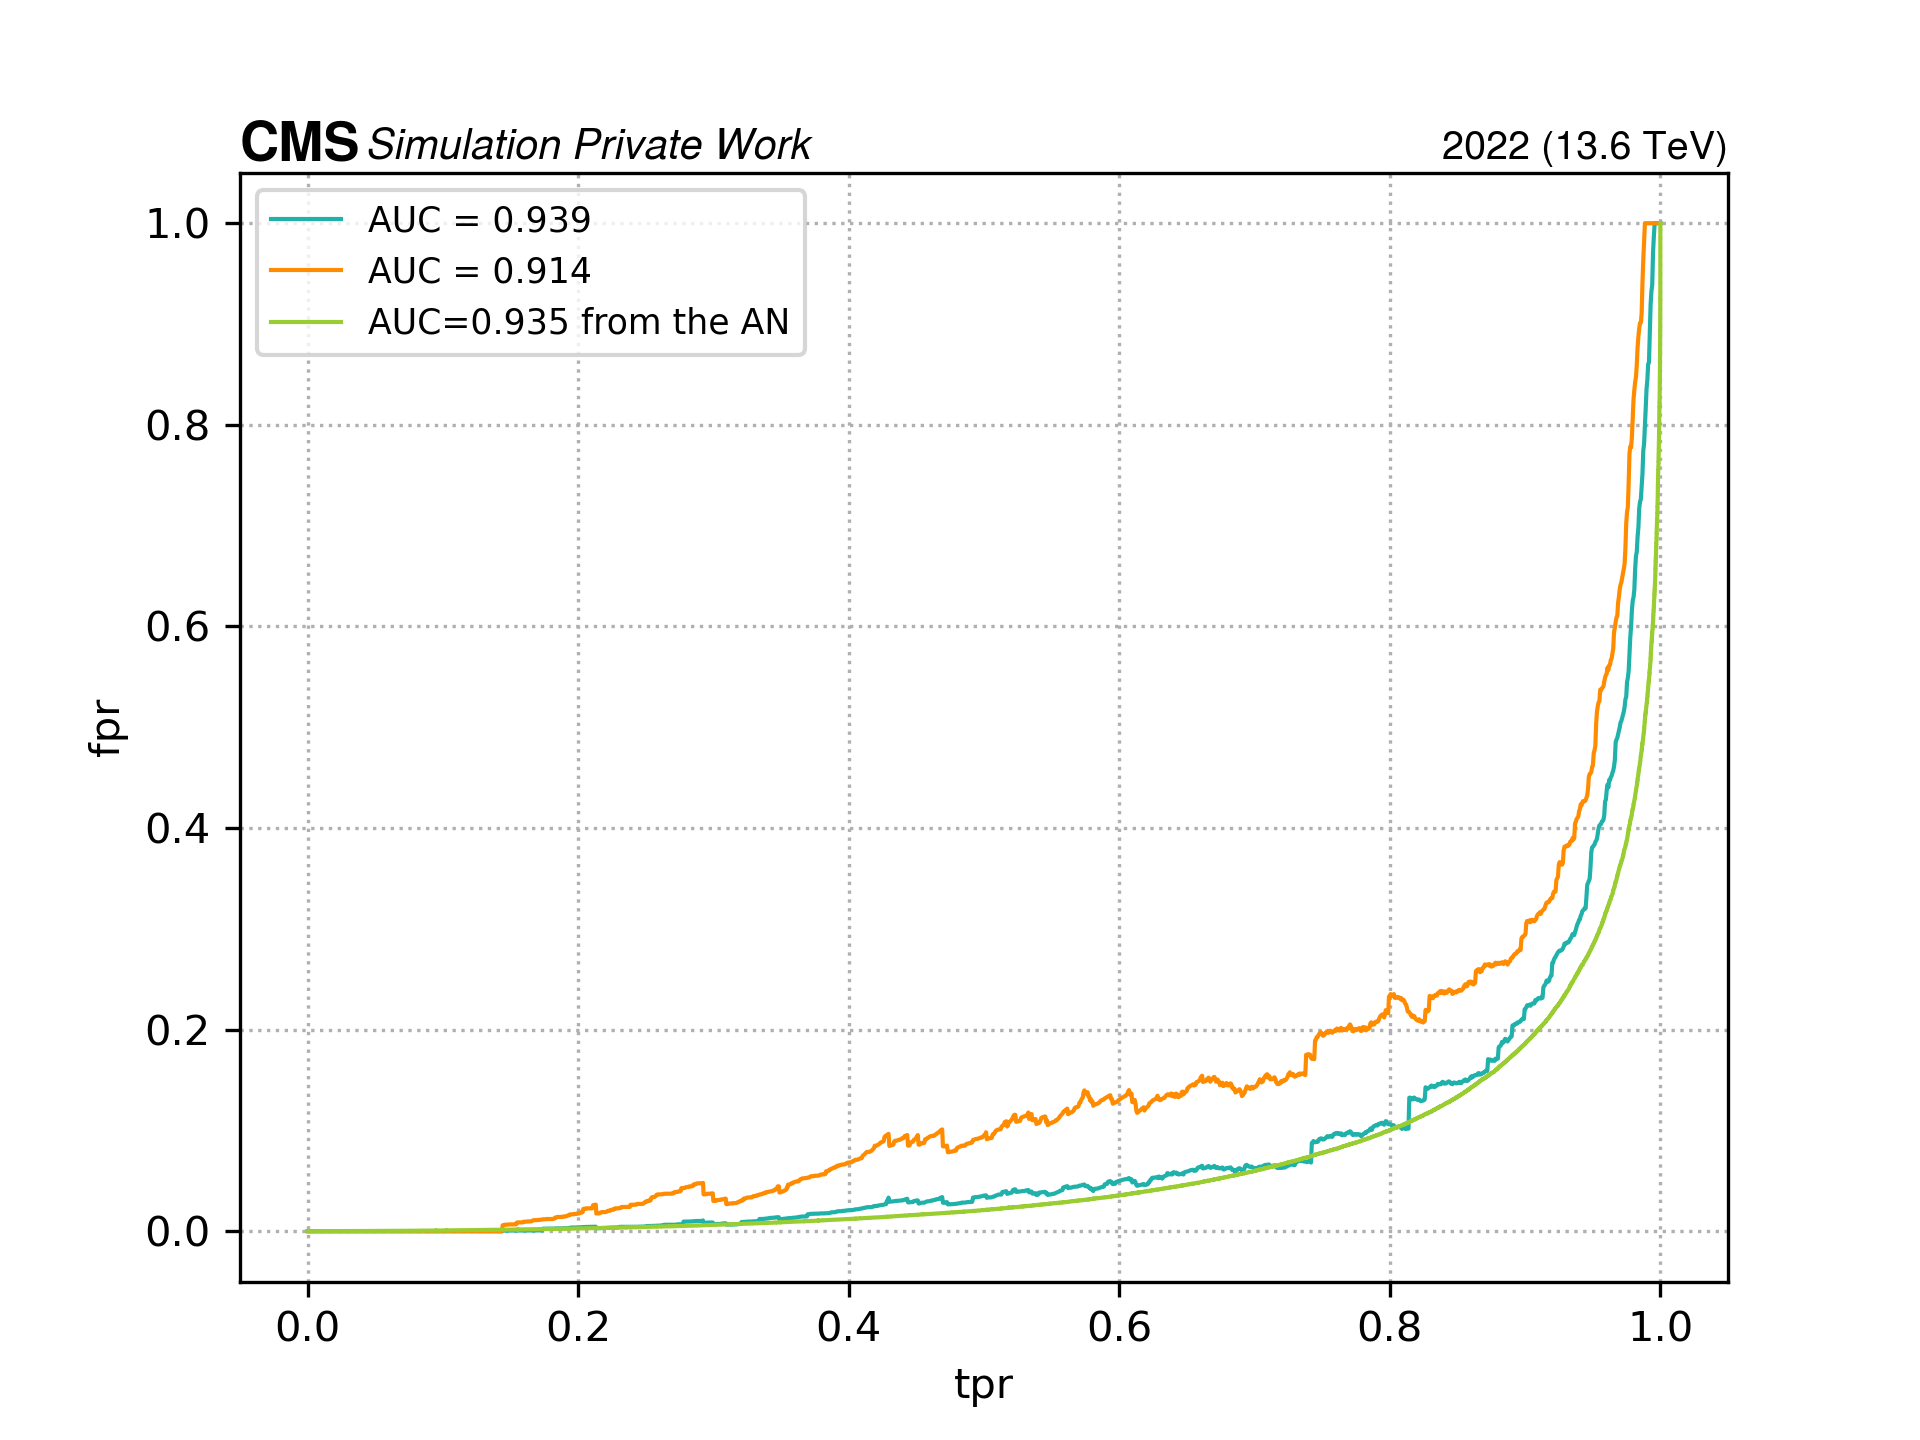
\includegraphics[width=0.7\linewidth]{Images/7.S:B/SR stats/4b data extrapolation dnn proba ev on sr.png}
    \caption{ROC curve inferred for 4b-data using the inclusive trainings with DNN and PD as inputs to compute FPR using Eq.(\ref{eq: extrapolation}). The TPR values are taken from the 2b data full statistics ROC curve. The AUCs showed in this Figure are inferred using Eq.(\ref{eq: extrapolation}).}
    \label{fig: ev on SR dnn pd}
\end{figure}

\clearpage


\subsubsection{Training and evaluation on SR} \label{subsubsection: train and eev on SR}

When performing the trainings in the SR it is to point out that, as shown in Table \ref{table: SR efficiency}, the SR selection efficiency is low for the background, hence, we are left with very small background statistics.

\begin{table}[hbt]
\centering
\begin{tabular}{|M{3cm}||M{3.5cm}|M{3.5cm}|M{3.5cm}|}
 \hline
 Sample  & Number of events after preselections & Number of events in the SR & SR efficiency\\
 \hline
 \hline
 4b-Signal & 800k & 540k & 67\%\\
 \hline
 4b-QCD & 120k & 10k & 8\% \\
 \hline
 4b-data & 130k &  &  \\
 \hline
 \hline
 2b-Signal & 420k & & \\
 \hline
 2b-QCD & 4.4M & 220k & 5\% \\
 \hline
 2b-data & 5.9M & 470k & 8\% \\
 \hline
\end{tabular}
\caption{Signal region efficiency for the different configurations used for the SPANet trainings.}
\label{table: SR efficiency}
\end{table}

Figure \ref{fig: Assigned prob 4b QCD SR} shows the probability assigned by SPANet after performing a training with the 4b-QCD configuration using only events in the signal region, which will be referred to as the 4b-QCD-SR configuration. In this case, DNN and PD variables are used as inputs. When considering the weighted events, significant fluctuations in the background are observed due to the lack of statistics. This is reflected in the ROC curve of this distribution as observed in Figure \ref{fig: ROC of the assignment proba SR}.  The same feature is observed when using only DNN as input variables.

\begin{figure}[hbt]
    \centering
    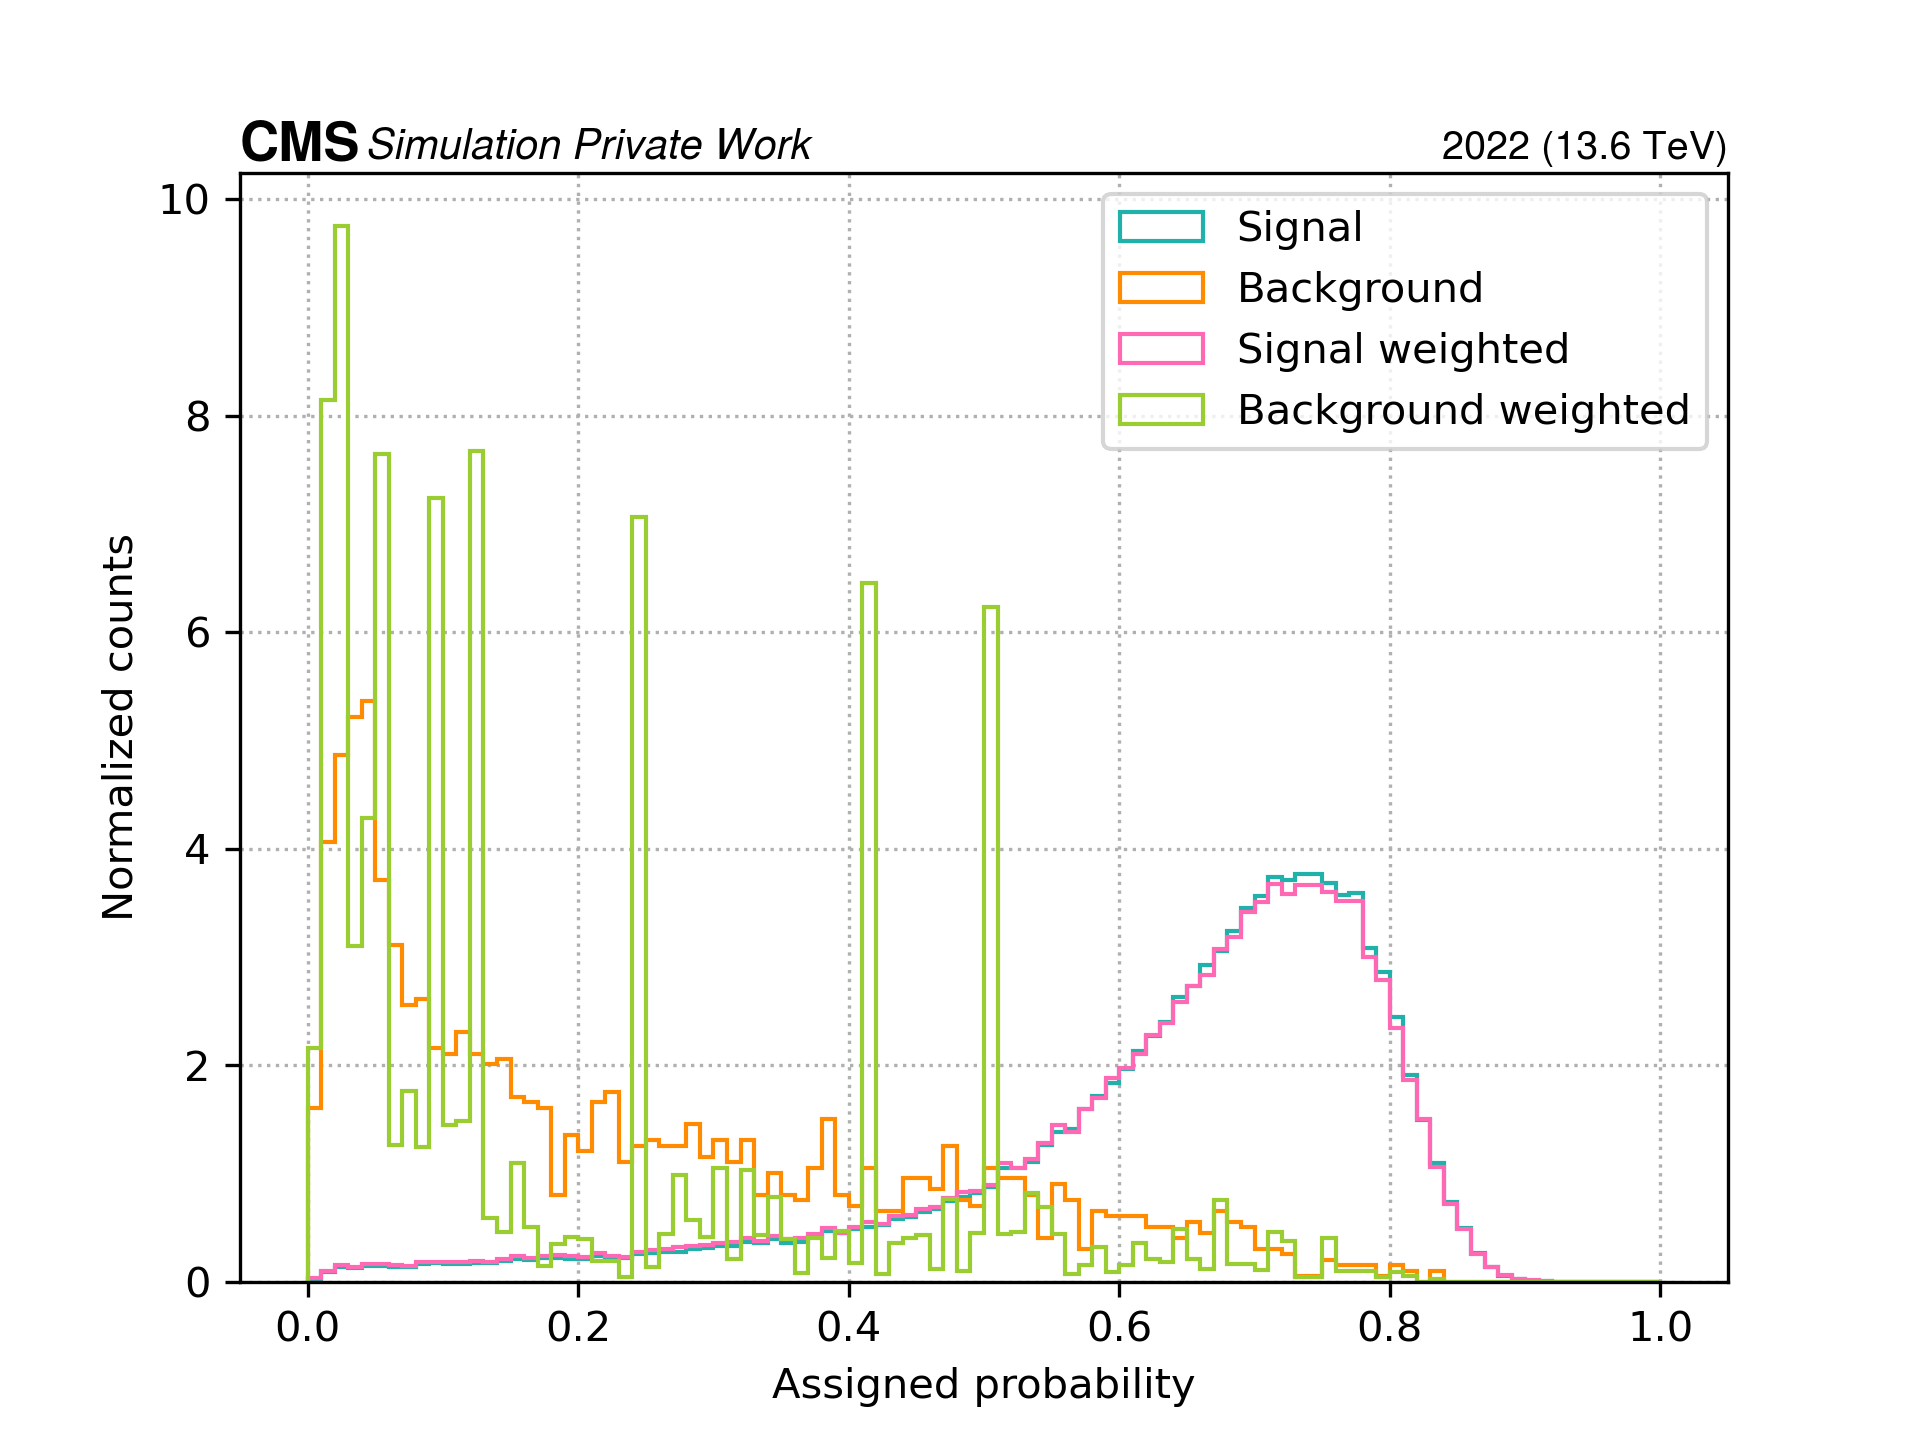
\includegraphics[width=0.7\linewidth]{Images/7.S:B/SR stats/4b stats SR class output.png}
    \caption{Probability assigned by SPANet as a classifier of the signal events in the SR as well as the 4b QCD background events in the signal region. For this training we used DNN and PD variables as global inputs. Due to the lack of statistics in the background, we observe large fluctuations in the background weighted distribution.}
    \label{fig: Assigned prob 4b QCD SR}
\end{figure}

\begin{figure}[hbt]
    \centering
    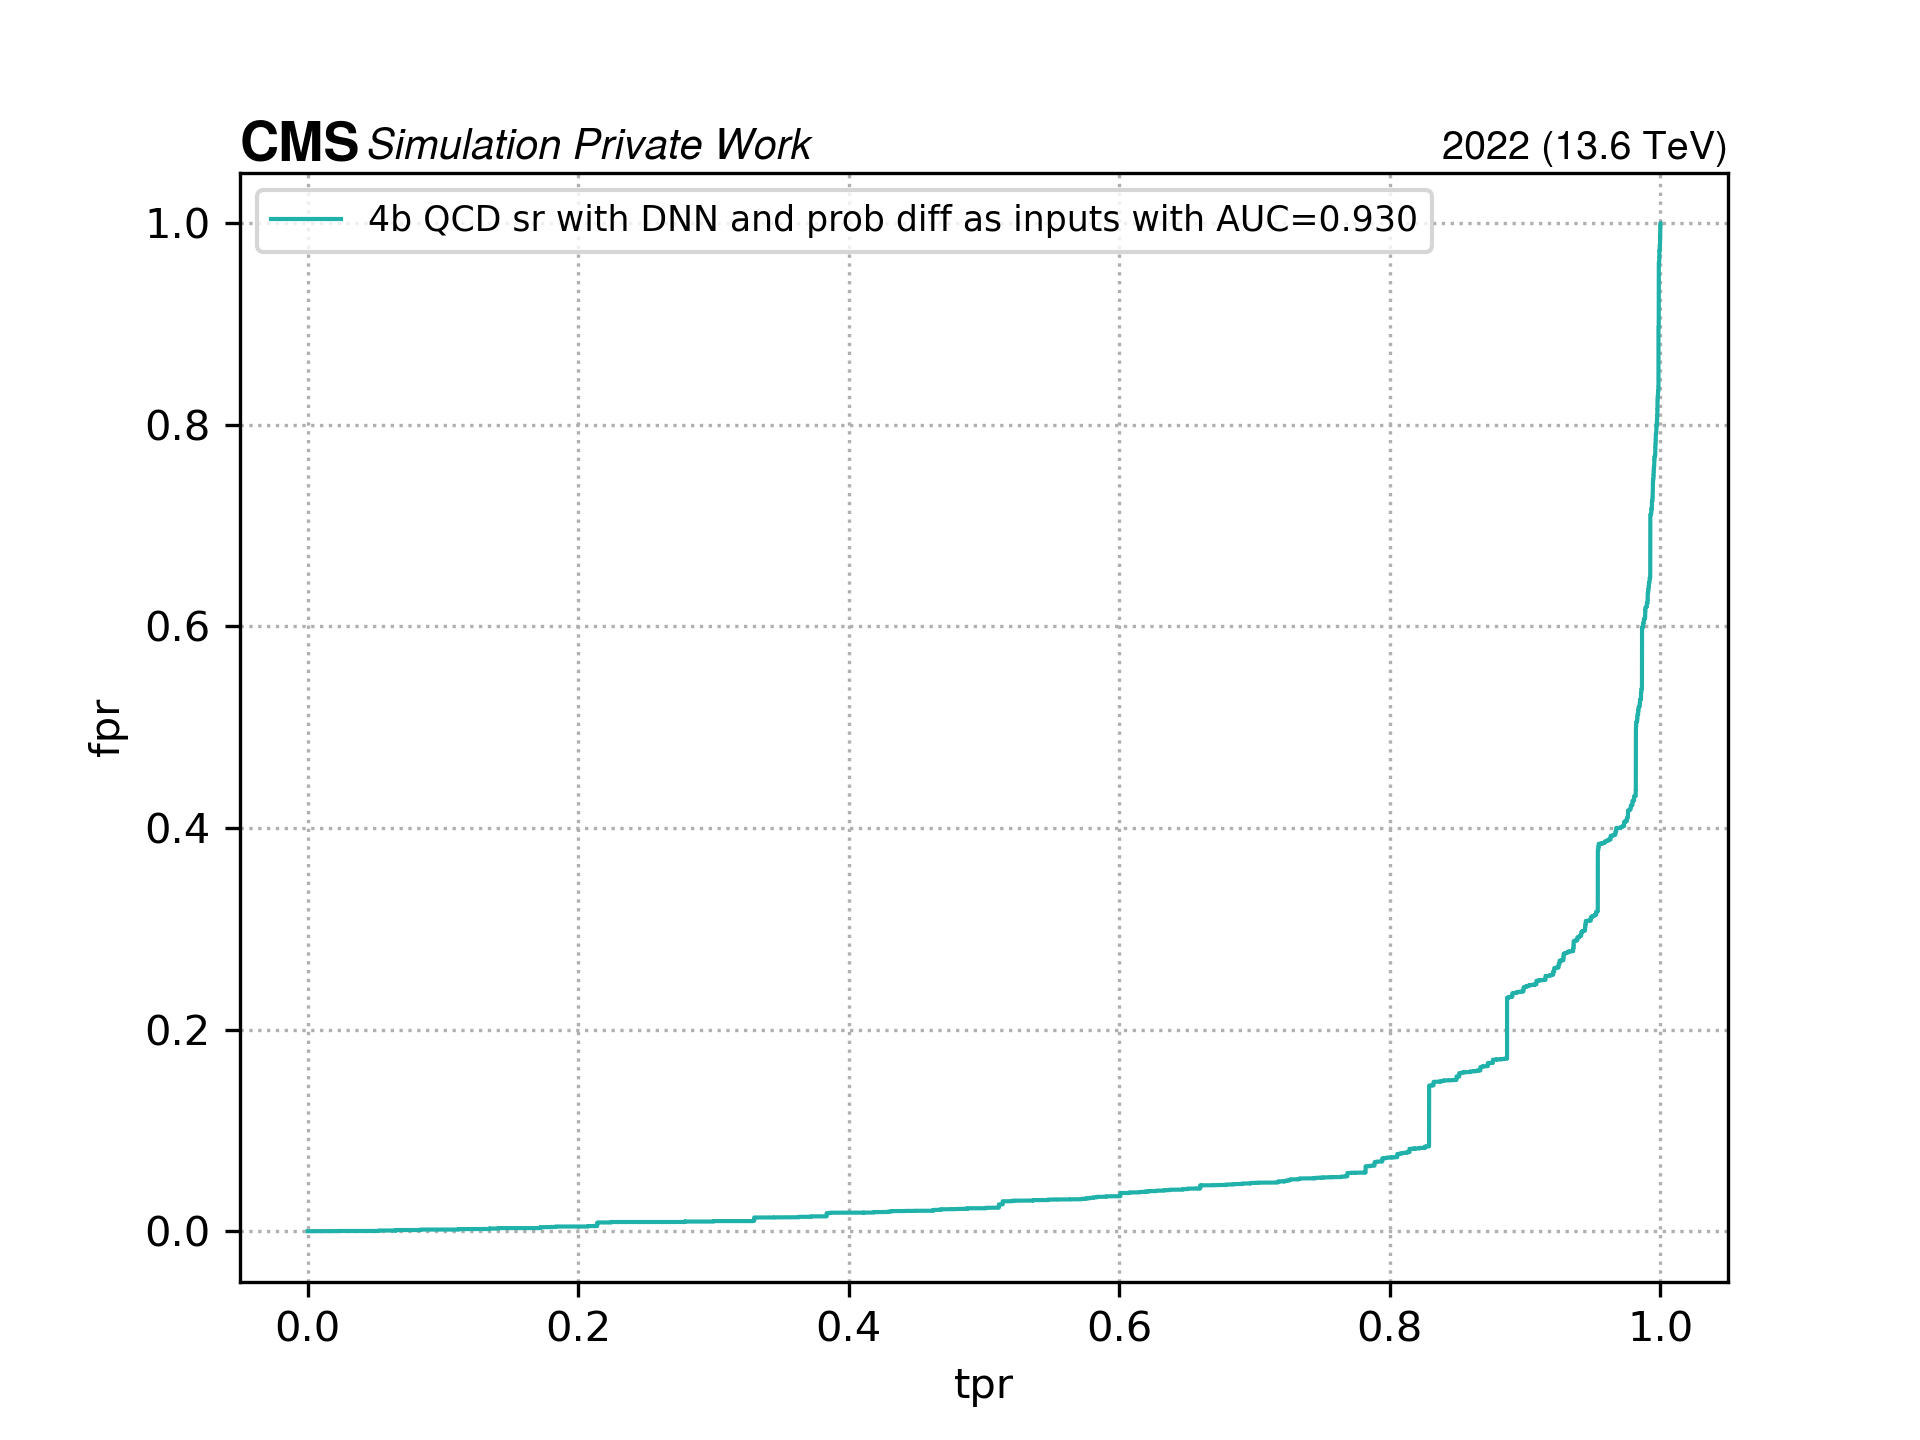
\includegraphics[width=0.7\linewidth]{Images/7.S:B/SR stats/ROC 4b QCD SR dnn proba.png}
    \caption{ROC of the assignment probability distribution obtained after a training and evaluation on SR samples shown in Figure \ref{fig: Assigned prob 4b QCD SR}.}
    \label{fig: ROC of the assignment proba SR}
\end{figure}

In Section \ref{subsection: var of training S/B} a large variability is observed for the 4b-QCD configuration, therefore the variability of trainings using the 4b-QCD-SR configuration is also tested. The outcome of these trainings is shown in Figure \ref{fig: 4b QCD SR variability} and in Table \ref{table: Spread of 4b QCD SR} the results are summarized. 

\begin{figure}[hbt]
\centering
\begin{subfigure}{.5\textwidth}
  \centering
  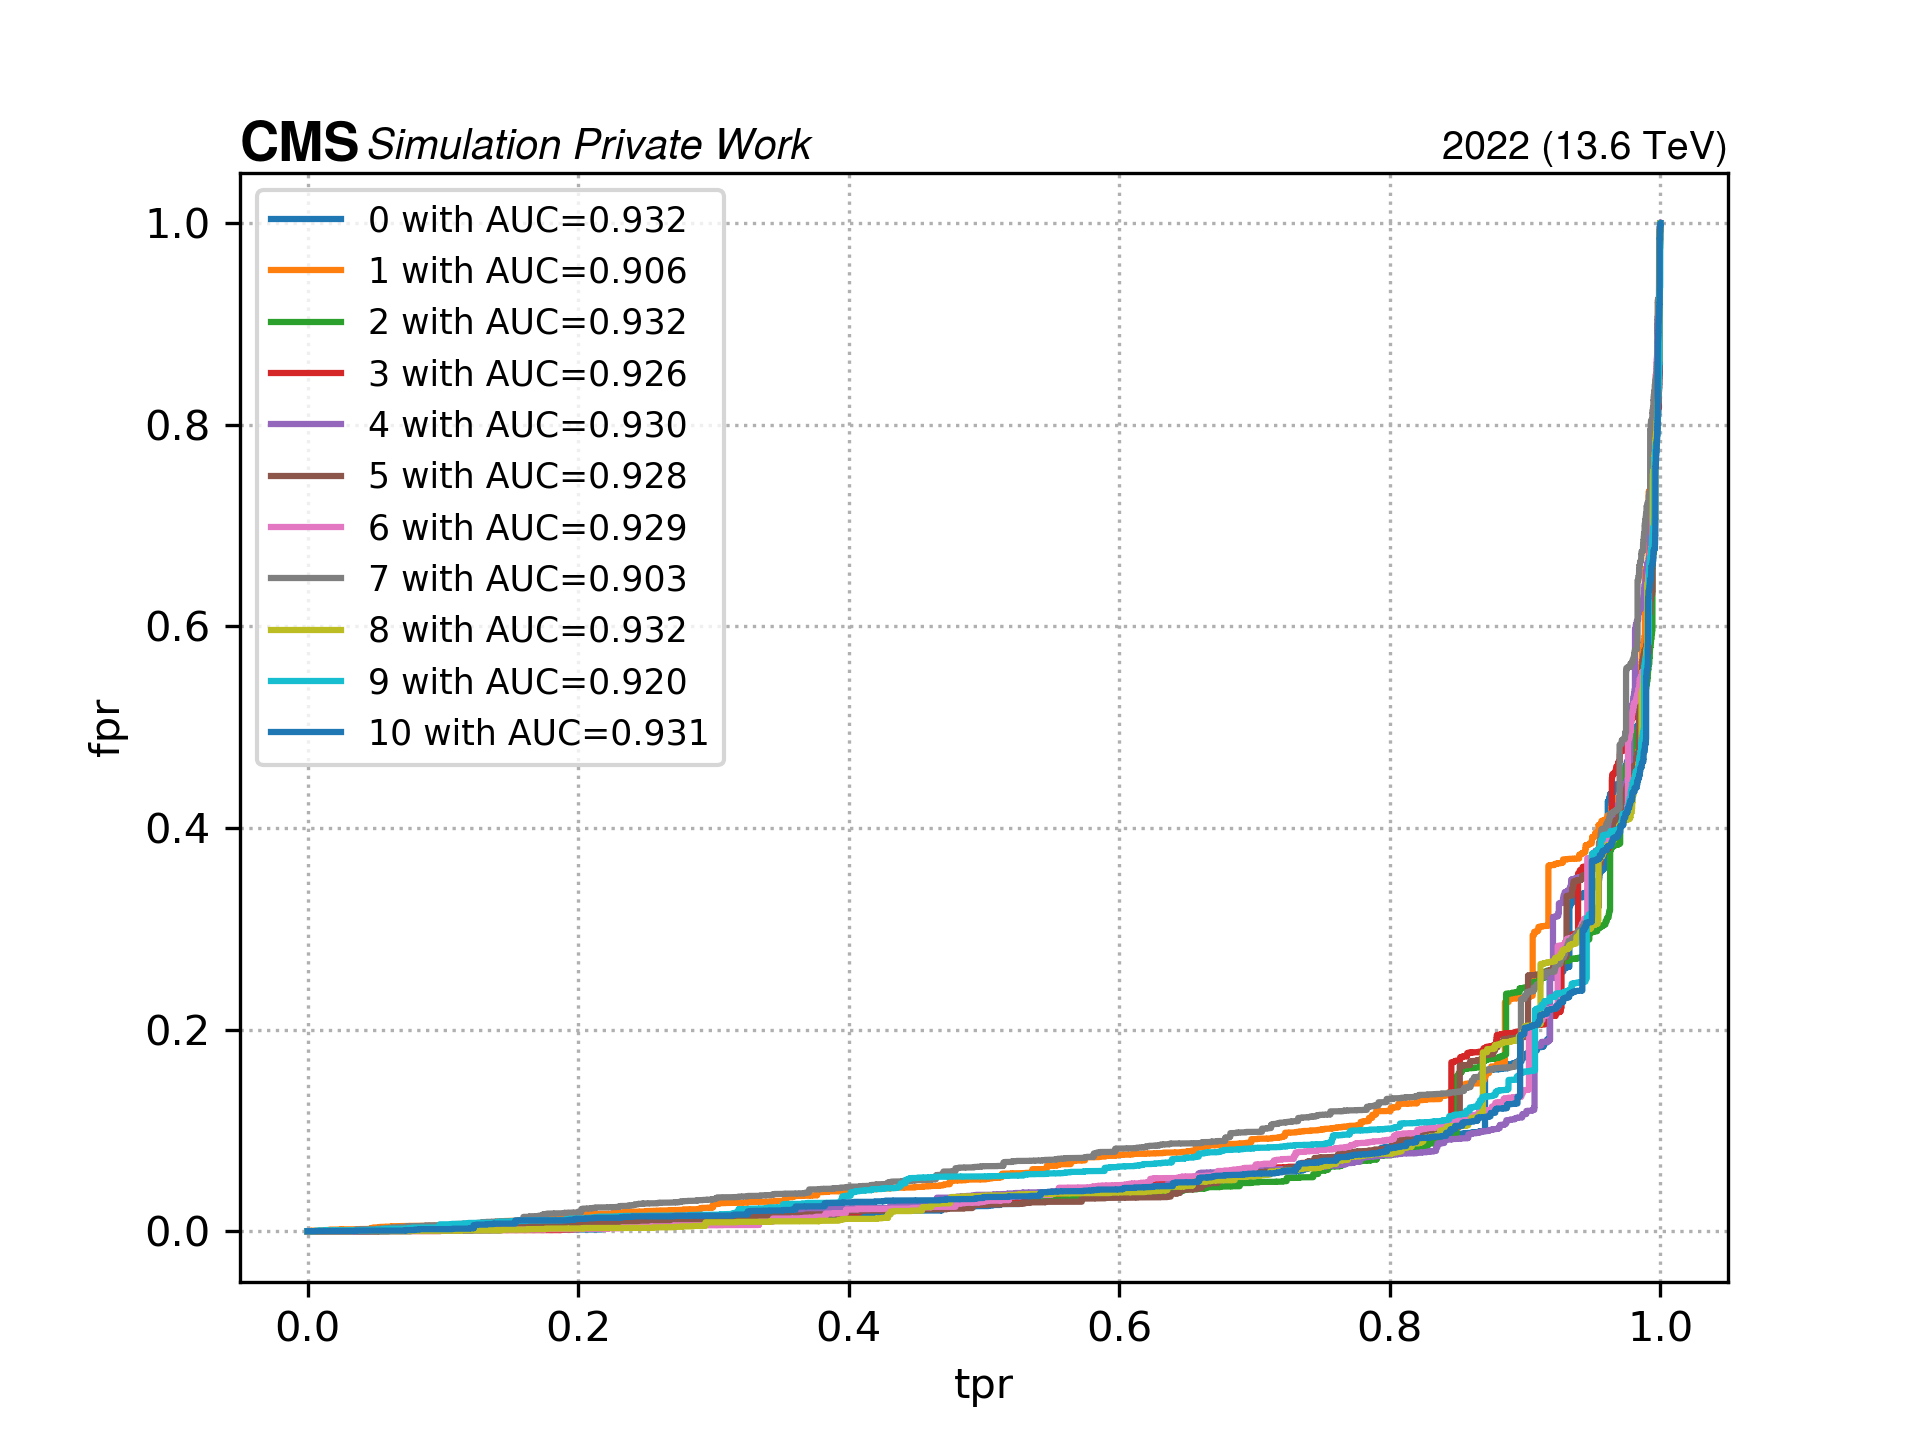
\includegraphics[width=1.1\linewidth]{Images/7.S:B/Variability/4b QCD sr dnn.png}
  \caption{DNN as global input}
  \label{fig: 4b QCD SR DNN}
\end{subfigure}%
\begin{subfigure}{.5\textwidth}
  \centering
  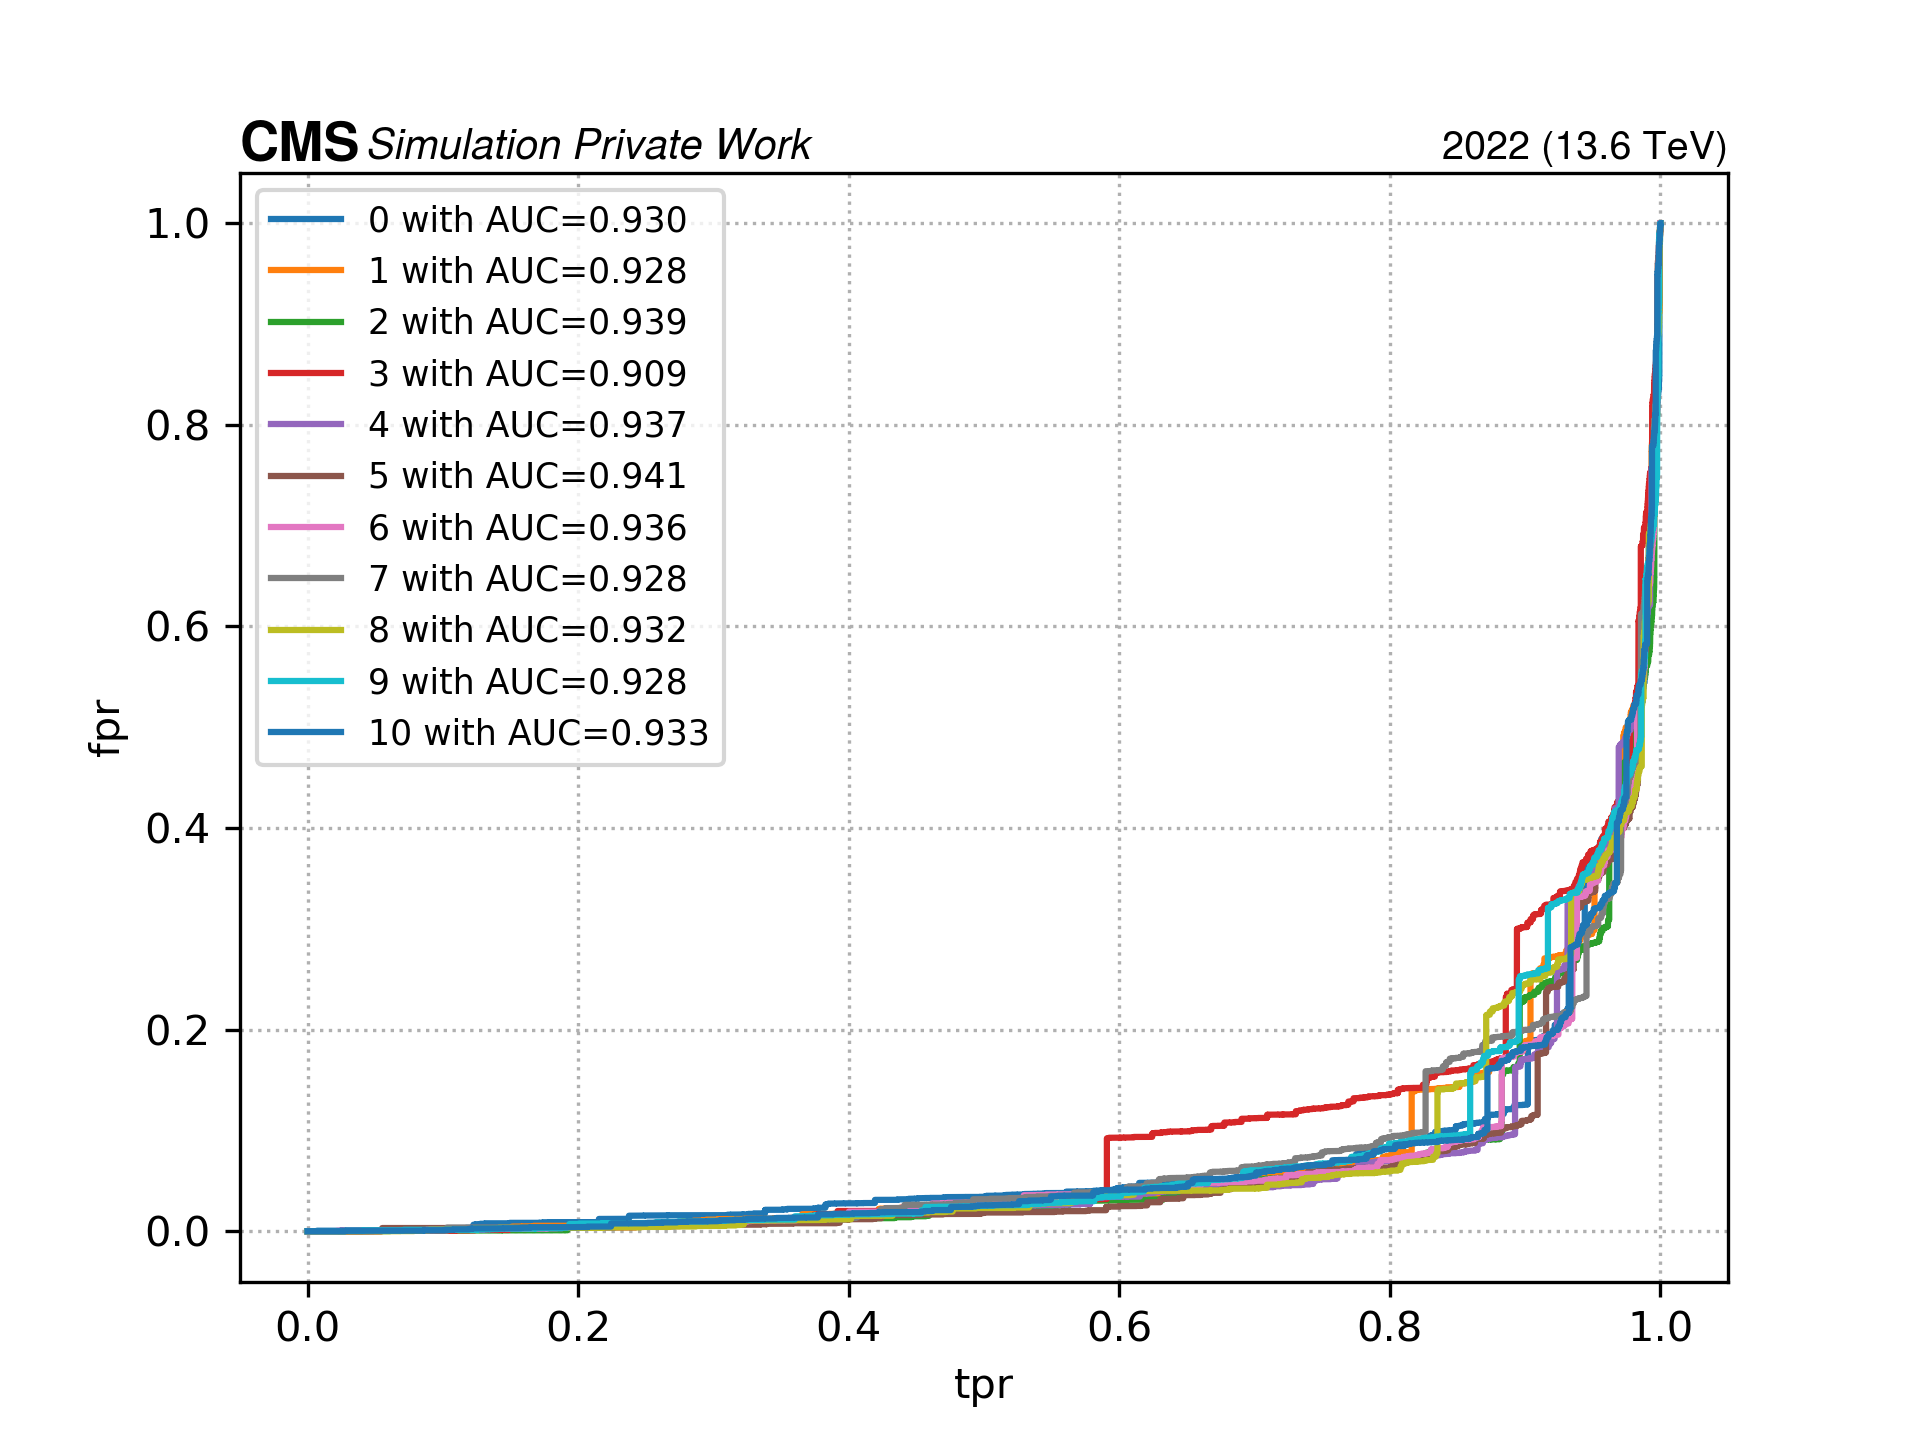
\includegraphics[width=1.1\linewidth]{Images/7.S:B/Variability/4b QCD sr dnn + prob diff.png}
  \caption{DNN and PD as global inputs}
  \label{fig: 4b QCD SR DNN PD}
\end{subfigure}
\caption{ROC curves produced by fixing eleven different seeds using 4b-QCD-SR and as inputs either DNN variables or DNN and PD variables. The AUC of each ROC curve are also reported in these Figures. The number next to the value of the AUC corresponds to the value of the seed fixed for the training.}
\label{fig: 4b QCD SR variability}
\end{figure}

\begin{table}[hbt]
\centering
\begin{tabular}{|M{5cm}||M{2.5cm}|M{2.5cm}|M{2.5cm}|}
 \hline
 Configuration  & Maximum value of the AUC & Minimum value of the AUC & Spread \\
 \hline
 4b-QCD-SR (DNN) & 0.932 & 0.903 & $\sim$0.029 \\
 \hline
 4b-QCD-SR (DNN and PD) & 0.941 & 0.909 & $\sim$0.033 \\
 \hline
\end{tabular}
\caption{Variability of the ROC and AUC values of the training for 4b-QCD SR training.}
\label{table: Spread of 4b QCD SR}
\end{table}

As shown in Table \ref{table: Spread of 4b QCD SR}, a higher variability is observed for the 4b-QCD-SR trainings than the one presented in Section \ref{subsection: var of training S/B}, which can be explained by the lack of statistics of the background. Therefore, to infer the ROC curve in the 4b-data, the same procedure explained in Section \ref{subsection: var of training S/B} is used. The b-tag ratio in Eq.(\ref{eq: extrapolation}) for the 11 seeds is computed and it is checked where the value from the AN
lies within this variability. The results are shown in Figures \ref{fig: 4b QCD SR DNN PD roc} and \ref{fig: 4b QCD SR DNN roc}. It is observed that although adding the PD variable as input increases the variability, it significantly improves the performance of the classification.

\begin{figure}[hbt]
    \centering
    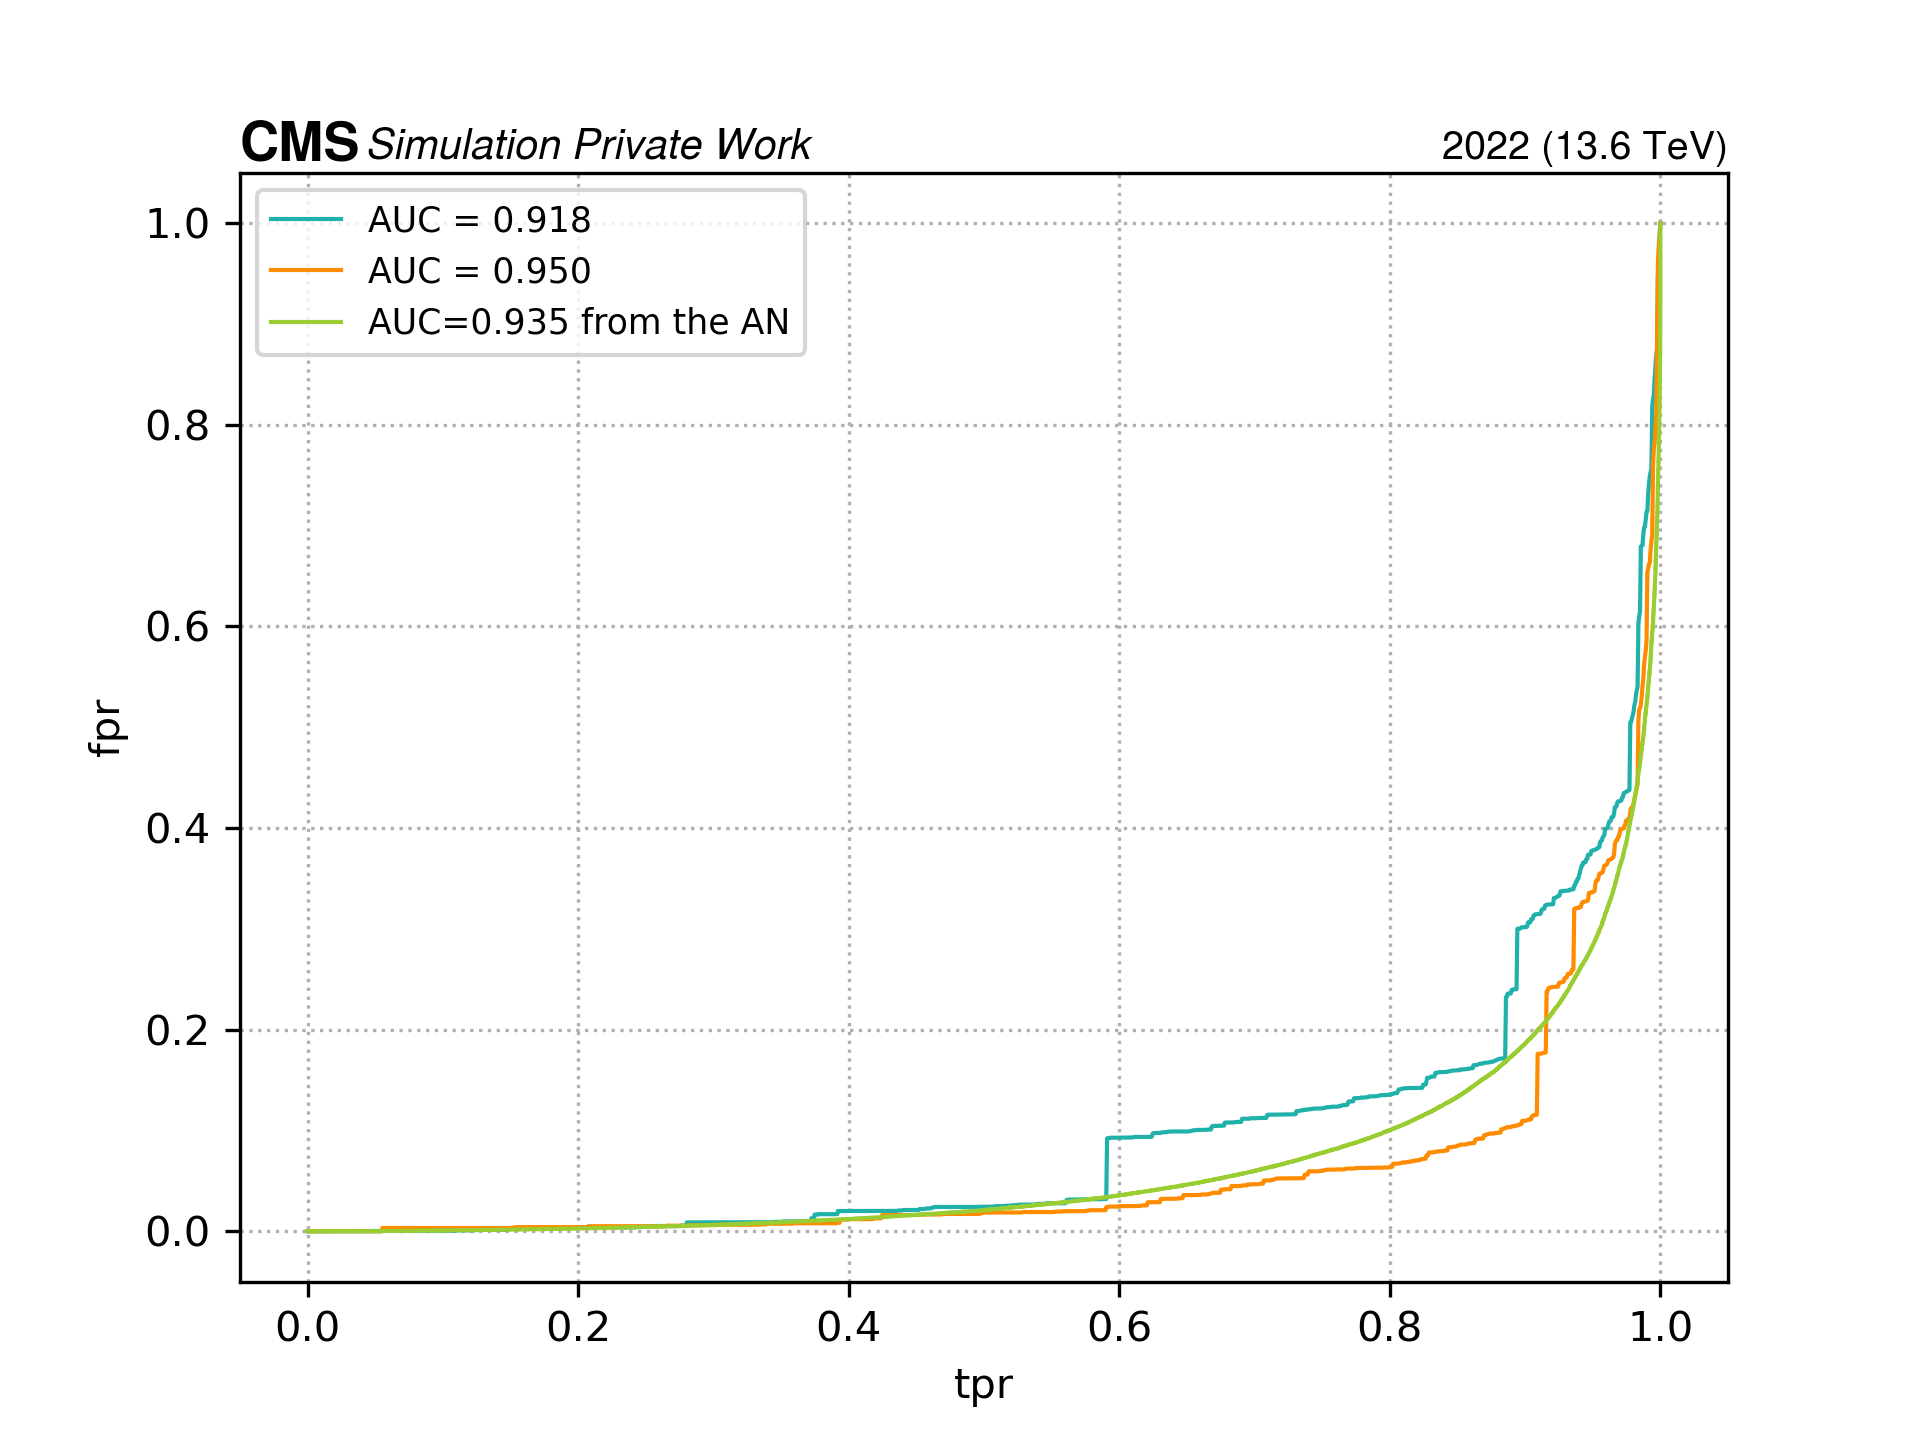
\includegraphics[width=0.7\linewidth]{Images/7.S:B/SR stats/4b data DNN + pb sr.png}
    \caption{ROC curve inferred for 4b-data in SR, with DNN, and PD as inputs, using Eq.(\ref{eq: extrapolation}) to compute the FPR and the TPR is taken from 2b data full statistics in SR ROC curve. The AUCs shown in this Figure are inferred using Eq.(\ref{eq: extrapolation}). Only the best and the worst performing trainings are shown in this figure to clearly show the performance bands inside which the AN ROC lies for better readability and comparison.}    
    \label{fig: 4b QCD SR DNN PD roc}
\end{figure}

\begin{figure}[hbt]
    \centering
    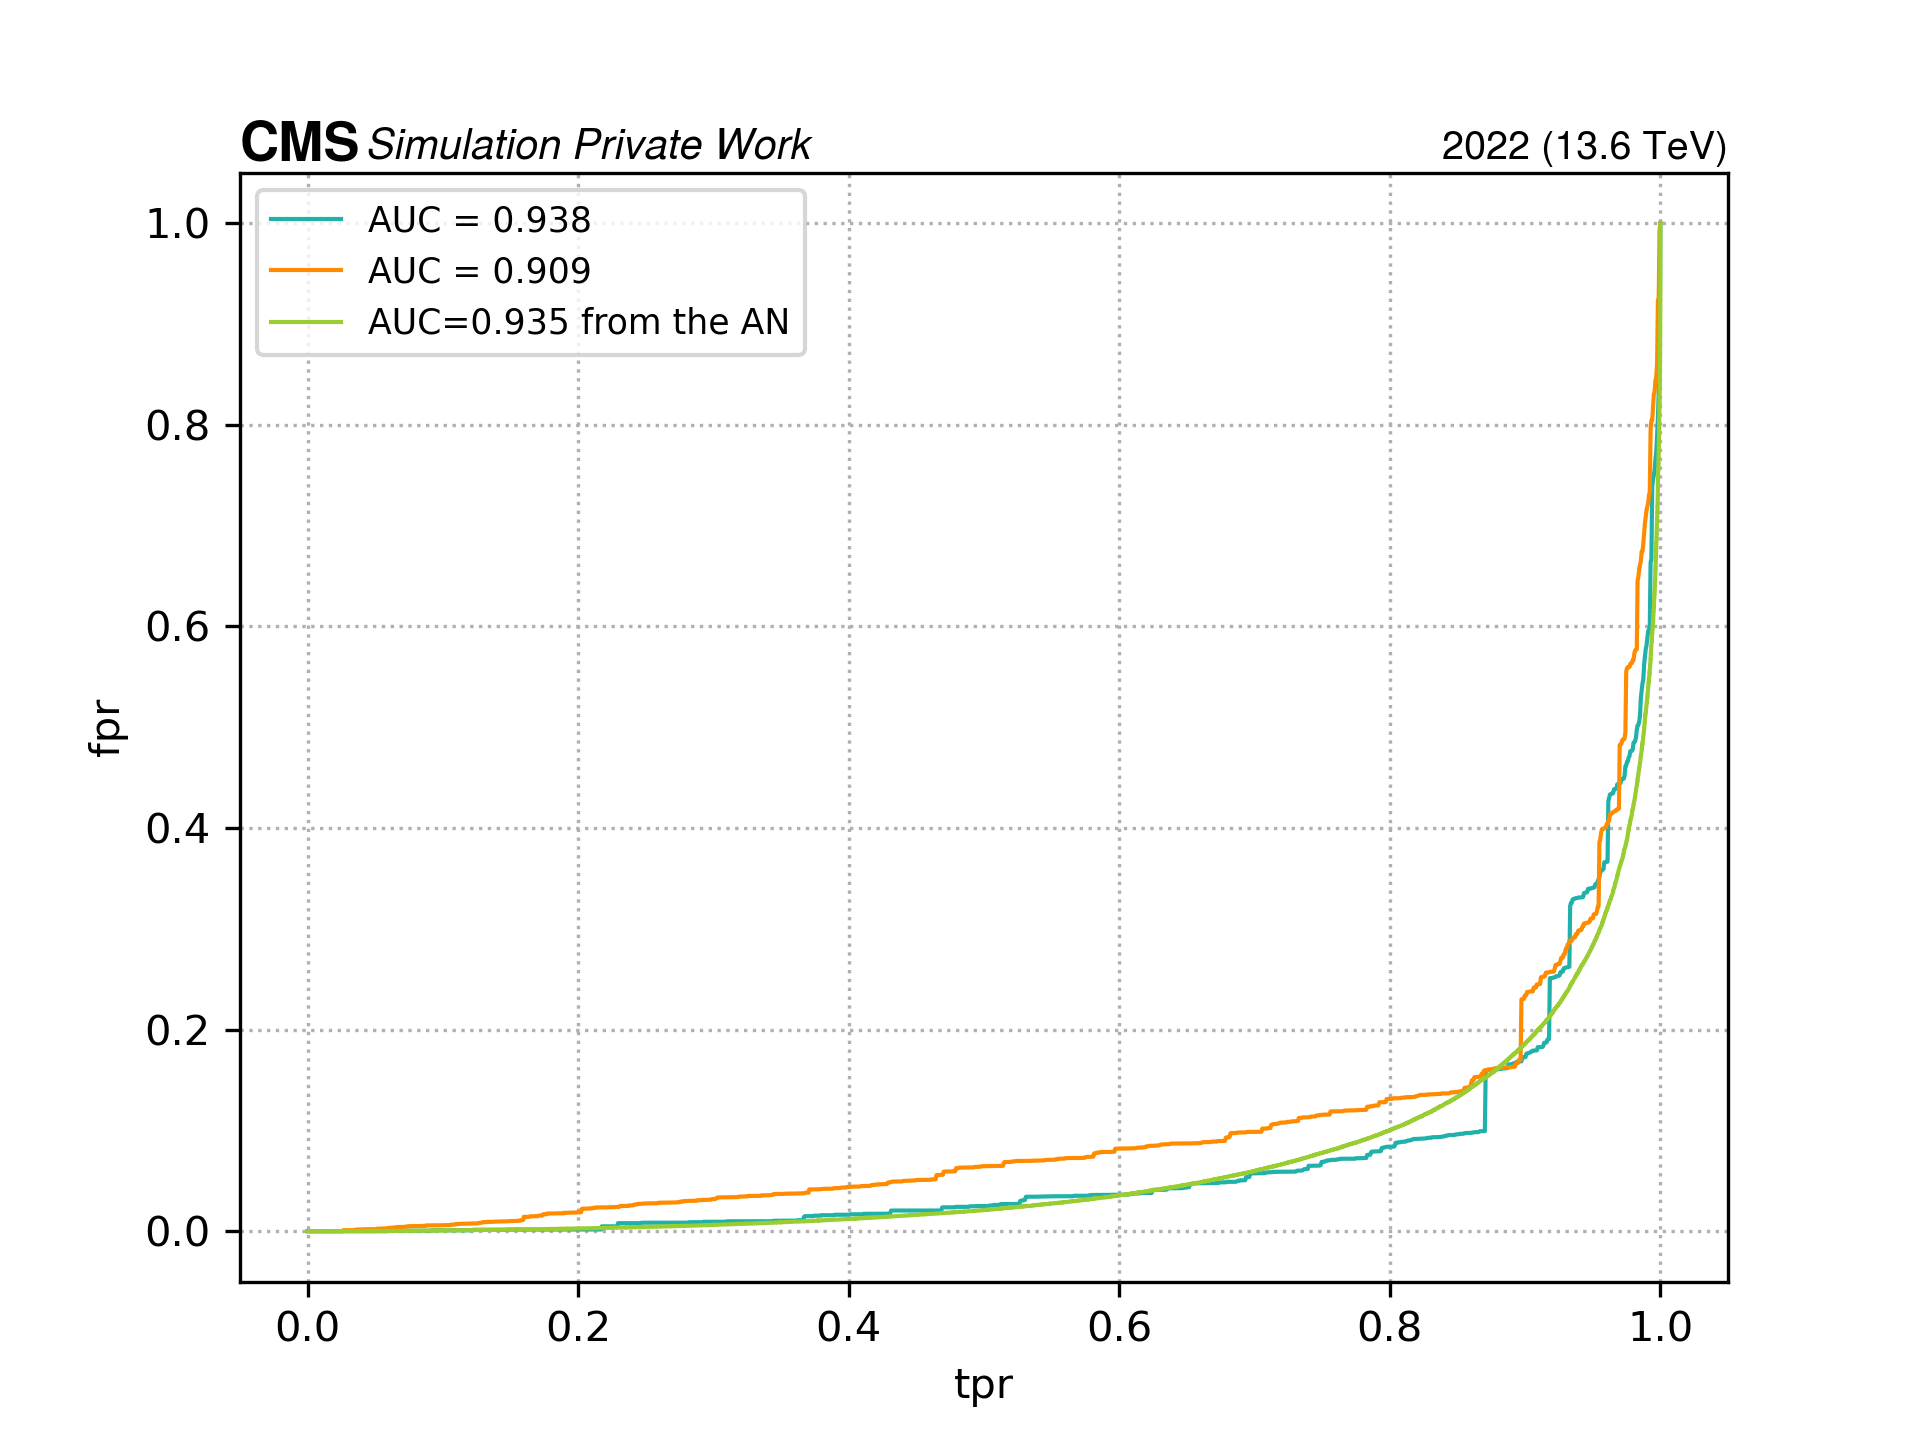
\includegraphics[width=0.7\linewidth]{Images/7.S:B/SR stats/4b data DNN.png}
    \caption{ROC curve inferred for 4b-data in SR, with DNN, and PD as inputs, using Eq.(\ref{eq: extrapolation}) to compute the FPR and the TPR is taken from 2b data full statistics in SR ROC curve. The AUCs shown in this Figure are inferred using Eq.(\ref{eq: extrapolation}). Only the best and the worst performing trainings are shown in this figure to clearly show the performance bands inside which the AN ROC lies for better readability and comparison.}
    \label{fig: 4b QCD SR DNN roc}
\end{figure}

We conclude (as shown in Table \ref{table: highest/ lowest SR 4b data}) that by training the SPANet model using the DNN and PD as global inputs, the smallest gain that we extract from this method is given by a difference of 0.015 in the AUC. Moreover, by using this training, the SPANET classification worse performance does not outperform the DNN used in Run 3, but is still better than the one using only DNN variables as global inputs. 

Comparing Figures \ref{fig: 4b QCD SR DNN PD roc} and \ref{fig: 4b QCD SR DNN roc} as a function of the TPR shows that the performance of the DNN for Run 3 is outperformed by the novel SPANet training up to 85\% signal efficiency. After this threshold on the signal efficiency at 85\%, the probability distribution given by SPANet is dominated by the background, therefore the lack of statistics plays a significant role.


In order to further improve the SPANet classification performance in the SR, it is proposed to oversample the 4b-QCD-SR sample used for the training. In this case, the oversampling consists of randomly shuffling the events in the 4b-QCD-SR sample and repeatedly concatenating them until the number of events is equal to the one in the 2b-data full statistics sample ($\sim$ 5M events).

\begin{table}[hbt]
\centering
\begin{tabular}{|M{5cm}||M{2.5cm}|M{2.5cm}|}
 \hline
 Configuration  & Maximum value of the AUC & Minimum value of the AUC \\
 \hline
 4b-data-SR (DNN) & 0.938 & 0.909  \\
 \hline
 4b-data-SR (DNN and PD) & 0.950 & 0.918 \\
 \hline
\end{tabular}
\caption{Comparison of the highest and lowest extrapolated AUC values for 4b-data using Eq.(\ref{eq: extrapolation}) to compute them.}
\label{table: highest/ lowest SR 4b data}
\end{table}

\begin{figure}[hbt]
    \centering
    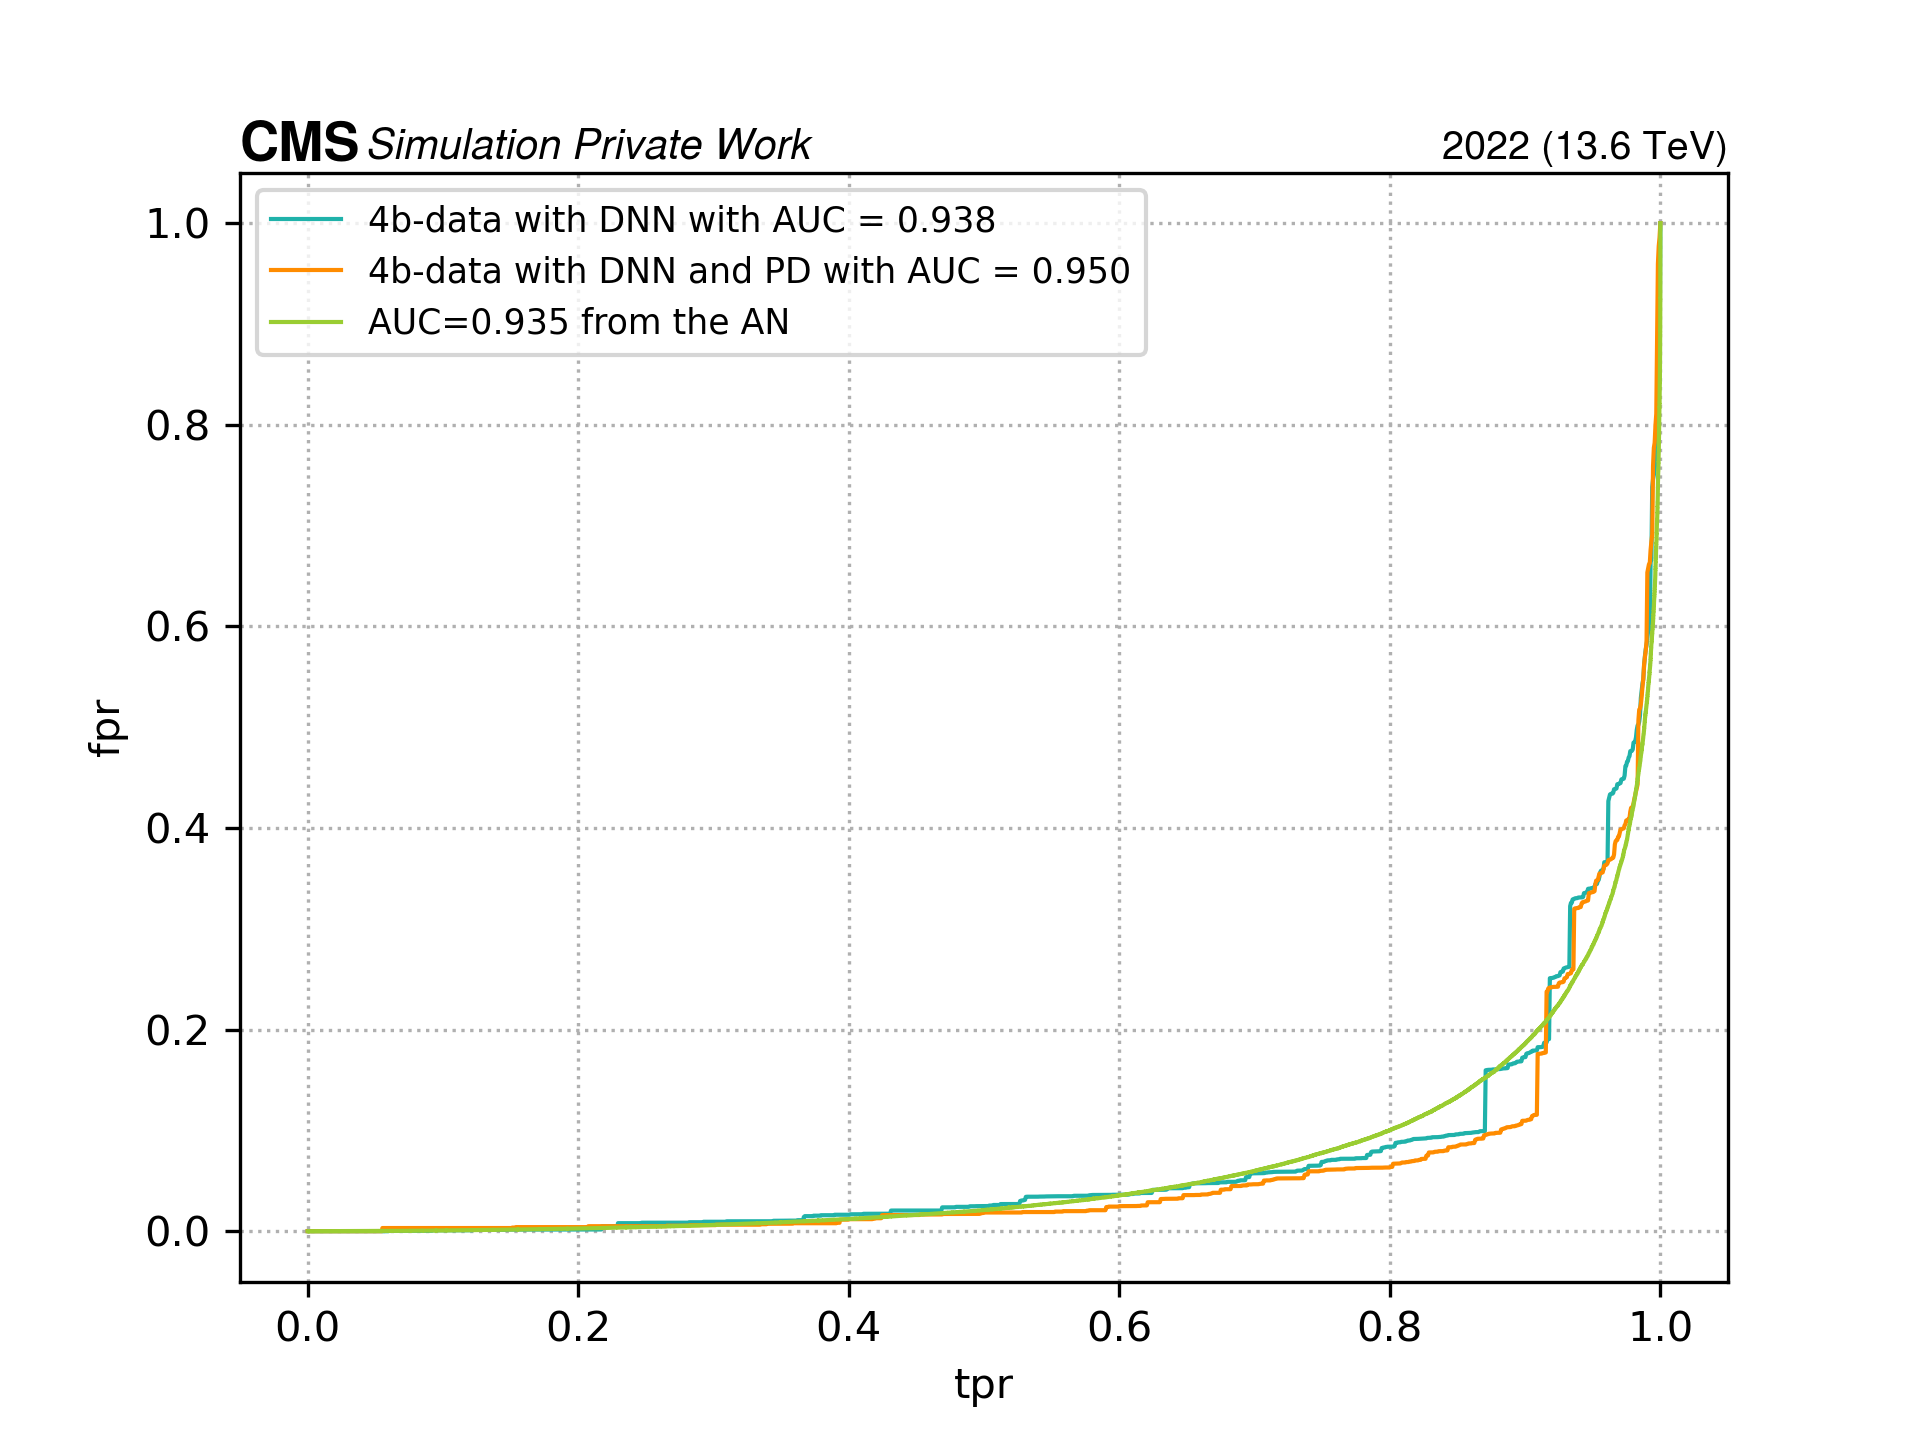
\includegraphics[width=0.7\linewidth]{Images/7.S:B/SR stats/HIghest AUC ROC vs Highest AUC vs AN.png}
    \caption{Comparison of the best performing inferred 4b-data-SR ROC curves when using either DNN as input variables or DNN as PD variables. The AUCs shown in this Figure are inferred using Eq.(\ref{eq: extrapolation}). This is the smallest possible gain for the best SPANET training configuration which shows that the benchmark results of the AN are outperformed by the novel SPANET training.}
    \label{fig: highest comp}
\end{figure}

\begin{figure}[hbt]
    \centering
    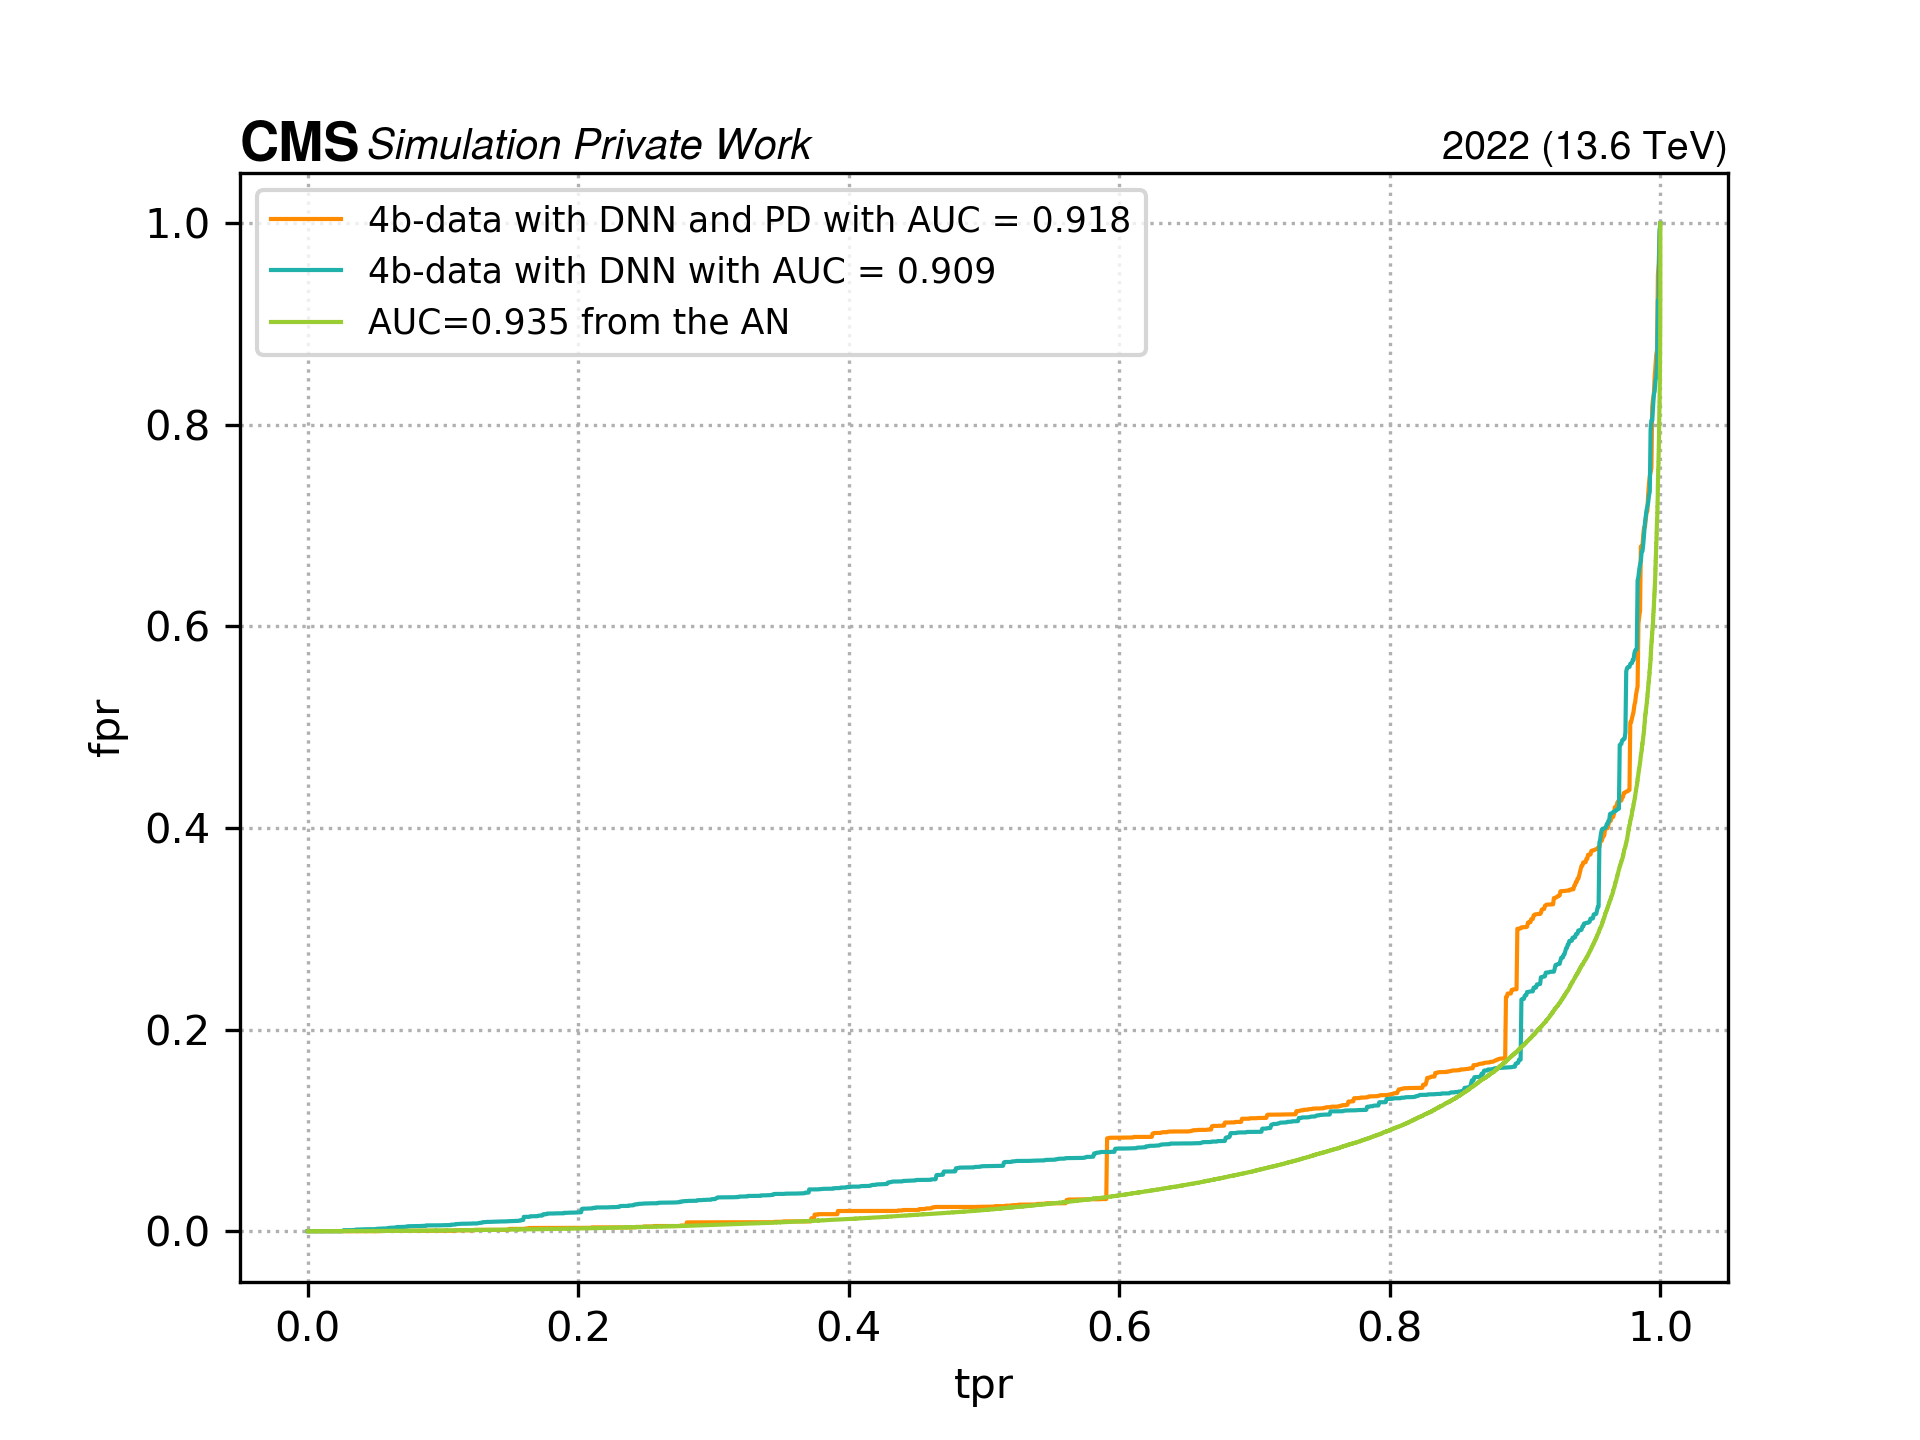
\includegraphics[width=0.7\linewidth]{Images/7.S:B/SR stats/lowest comp 4b data.png}
    \caption{Comparison of the worst performing inferred 4b-data-SR ROC curve when using either DNN as input variables or DNN as PD variables. The AUCs showed in this Figure are the inferred using Eq.(\ref{eq: extrapolation}).}
    \label{fig: lowest comp}
\end{figure}
